\newcommand{\xin}{\mathbf{x}_{\texttt{in}}}
\newcommand{\xini}{x_{\texttt{in}_i}}
\newcommand{\xout}{\mathbf{x}_{\texttt{out}}}
\newcommand{\xoutj}{x_{\texttt{out}_j}}
\newcommand{\Xin}{\mathbf{X}_{\texttt{in}}}
\newcommand{\Xini}{\mathbf{X}_{\texttt{in}_i}}
\newcommand{\Xout}{\mathbf{X}_{\texttt{out}}}
\newcommand{\Xoutj}{\mathbf{X}_{\texttt{out}_j}}
\newcommand{\XinOne}{\mathbf{X}_{\texttt{in}_1}}
\newcommand{\XinN}{\mathbf{X}_{\texttt{in}_N}}
\newcommand{\Xoutjk}{X_{\texttt{out}_{jk}}}
\newcommand{\Xinik}{X_{\texttt{out}_{ik}}}

\newcommand{\tin}{\mathbf{t}_{\texttt{in}}}
\newcommand{\tini}{t_{\texttt{in}_i}}
\newcommand{\tout}{\mathbf{t}_{\texttt{out}}}
\newcommand{\touti}{t_{\texttt{out}_i}}

\newcommand{\Zin}{\mathbf{Z}_{\texttt{in}}}
\newcommand{\Zout}{\mathbf{Z}_{\texttt{out}}}

\newcommand{\Qin}{\mathbf{Q}_{\texttt{in}}}
\newcommand{\Kin}{\mathbf{K}_{\texttt{in}}}
\newcommand{\Vin}{\mathbf{V}_{\texttt{in}}}

\definecolor{param_color}{rgb}{0.2, 0.6, 1.0}
\definecolor{data_color}{rgb}{1.0, 0.4, 0.38}

\usetikzlibrary{arrows,arrows.spaced,decorations.markings,calc}
\pgfplotsset{colormap/viridis}

\definecolor{gray_neuron}{rgb}{0.7,0.7,0.7}
\definecolor{param_color}{rgb}{0.2, 0.6, 1.0}
\definecolor{data_color}{rgb}{1.0, 0.4, 0.38}

\definecolor{query_color}{rgb}{0.94, 0.73, 0.247}
\definecolor{key_color}{rgb}{0.73, 0.23, 0.474}
\definecolor{value_color}{rgb}{0.29, 0.647, 0.615}

\definecolor{query_color_bright}{rgb}{0.1, 0.93, 0.447}
\definecolor{key_color_bright}{rgb}{0.93, 0.43, 0.674}
\definecolor{value_color_bright}{rgb}{0.49, 0.847, 0.815}

% https://tex.stackexchange.com/questions/27279/how-to-make-an-arrow-bigger-and-change-its-color-in-tikz/27287#27287
\tikzset{
  nn_edge/.style={
    decoration={markings,mark=at position 1 with {\arrow[scale=0.9]{spaced latex}}},
    postaction={decorate},
    shorten >=3.0pt
    }
  }

%\setcounter{chapter}{22}
\chapter{Transformers}\label{chapter:transformers}

%\textit{Draft chapter from Torralba, Isola, Freeman (this is a computer vision textbook, hence the emphasis on CNNs; note that transformers are also very related to GNNs)}

\section{Introduction}

{\bf Transformers} are a recent family of architectures that generalize and expand the ideas behind CNNs. The term for this family of architectures was coined by \cite{vaswani2017attention}, where they were applied to language modeling. Our treatment in this chapter more closely follows the ``Vision Transformers" introduced in \cite{dosovitskiy2020vit}.% but the general class includes many variations with a long history~\cite{XX,YY,ZZ}.

Like CNNs, transformers factorize the signal processing problem into stages that involve independent and identically processed chunks.\marginnote{Transformers were originally introduced in the field of natural language processing, where they were used to model language -- sequences of characters and words. As a result, some texts present transformers as an alternative to RNNs for sequence modeling, but in fact transformer layers are \textit{parallel} processing machines, like convolutional layers, rather than a sequential machine, like recurrent layers. Therefore, we will present transformers as more related to CNNs than RNNs. Transformers are also a special case of a more general architecture called ``graph neural networks", which we do not cover in this book.}[-0.4cm] However, they also include layers that mix information across the chunks, called ``attention layers", so that the full pipeline can model dependences between the chunks. %However, the way they do this is slightly more complicated than just cutting up the input tensor into patches.

%Transformers were introduced in \cite{vaswani2017attention} for natural language processing (NLP), although the technical components have a long history in the literature~\cite{XX,YY,ZZ}.

%Transformers can be understood as CNNs with additional layers -- which are called ``attention" layers -- inserted to mix information across across chunks.

\section{A limitation of CNNs: independence between far apart patches}
CNNs are built around the idea of \textit{locality}: different local regions of an image can safely be processed independently. This is what allows us to use filters with small kernels. However, very often, there is global information that needs to be shared across all receptive fields in an image. Convolutional layers are not well-suited to \textit{globalizing} information since the only way they can do so is by either increasing the kernel size of their filters, or by stacking layers to increase the receptive field of neurons on deeper layers.

How can we efficiently pass messages across large spatial distances? We already have seen one option: just use a fully-connected layer, so that every output neuron after this layer takes input from every neuron on the layer before. However, fully-connected layers have a ton of parameters -- $N^2$ if their input and output are $N$-dimensional vectors -- and it can take an exorbitant amount of time and data to fit all those parameters. Can we come up with a more efficient strategy?

%[Example image with different attention maps.]

\section{The idea of attention}
Attention is a strategy for processing global information efficiently, focusing just on the parts of the signal that are most salient to the task at hand. The idea can be motivated by attention in human perception. When we look at a scene, our eyes flick around and we ``attend to" certain elements that stand out, rather than taking in the whole scene at once~\cite{wolfe2000visual}. If we are asked a question about the color of a car in the scene, we will move our eyes to look at the car, rather than just staring passively. Can we give neural nets the same ability?

In neural nets, attention follows the same intuitive idea. A set of neurons on layer $l+1$ may \textit{attend} to a set of neurons on layer $l$, in order to decide what their response should be. If we ``ask" that set of neurons to report the color of any cars in the input image, then they should direct their attention to the neurons on the layer before that represent the color of the car. We will soon see how this is done, in full detail, but first we need to introduce a new data structure and a new way of thinking about neural processing. 

\section{A new data type: tokens}
We discussed that the main data structures in deep learning are different kinds of groups of neurons -- channels, tensors, batches, etc. Now we will introduce another fundamental data structure, {\bf tokens}. A ``token" is another kind of group of neurons, but there are particular ways we will operate over tokens that are different from how we operated over channels, batches, and the other groupings we saw before. Specifically,  we will think of tokens as \textit{encapsulated} groups of information; we will define operators over tokens, and these operators will be our only interface for accessing and modifying the internal contents of tokens. From a programming languages perspective, you can think of tokens as a new data \textit{type}.

%Therefore, we should think of tokens as a new data \textit{type}, with specific syntax and semantics. 

%\marginnote{Vectors of neurons are given different names and connotations in different contexts. In the context of representation learning, they are more commonly called ``embeddings".}[-1.0cm]

%At first it might not seem like we need a new term here, but the reason it's useful is because ``tokens" come with connotations about how we will use them. In particular, we will think of tokens as encapsulated groups of information; we will define operators over tokens, and these operators will be our only interface for accessing and modifying the internal contents of tokens.\marginnote{With this way of thinking, it's easy to imagine tokens that are any kind of structured group, rather than just being vectors of neurons. We just need to define how basic operators, like summation, operate over these groups (and, ideally, in a differentiable manner).}[-1.2cm] 

In this chapter we will only consider token whose internal content is a vector of neurons. We will call this vector the token's \textbf{code} vector; the code for a token $t$ will be labeled as $t.\mathbf{z}$.\marginnote{Although we are only considering vector-valued tokens in this chapter, it's easy to imagine tokens that are any kind of structured group. We just need to define how basic operators, like summation, operate over these groups (and, ideally, in a differentiable manner).}[-0.8cm] 
%Summing tokens and multiplying tokens by a scalar follows regular vector conventions over their codes; i.e. let $a$ and $b$ be tokens and $w$ be a scalar, then: 
%\begin{align}
%    a &\equiv [a.\mathbf{z}[1], \ldots, a.\mathbf{z}[N]]\\
%     b &\equiv [b.\mathbf{z}[1], \ldots, b.\mathbf{z}[N]]\\
%     a + b &\equiv [a.\mathbf{z}[1] + b.\mathbf{z}[1], \ldots, a.\mathbf{z}[N] + b.\mathbf{z}[N]]\\
%     wa &\equiv [a.\mathbf{z}[1]*w, \ldots, b.\mathbf{z}[N]*w]
% \end{align}

% , so a token $t$ has the form:
% \begin{align}
%     t = [z^t_1, \ldots, z^t_n]
% \end{align}
% Even though $t$ is a vector we will not bold it because we will think of the token as the atomic units of our computation, analogous to individual neurons. This will make it so the notation for working with tokens matches our notation for working with neurons. Just remember that each individual token actually contains within it a vector of values. For clarity, we will call this internal vector of values the token's \textbf{code} vector. Summing tokens and multiplying tokens by a scalar follows regular vector conventions over the codes, and multiplying two tokens takes their inner product of their codes (dot product); i.e. let $a$ and $b$ be tokens and $w$ be a scalar, then:
% \begin{align}
%     a + b &\equiv [a_1 + b_1, \ldots, a_n + b_n]\\
%     wa &\equiv [wa_1, \ldots, wa_n]\\
%     ab &\equiv \sum_i a_ib_i
% \end{align}

Transformers consist of two main operations over tokens: 1) \textit{mixing} tokens via a weighted sum, and 2) \textit{modifying} each individual token via a nonlinear transformation. These operations are analogous to the two workhorses of regular neural nets: the linear layer and the pointwise nonlinearity. Before we get to that, though, how do we turn data into tokens in the first place?

\subsection{Tokenizing data}
%The way to think about tokens is as discrete bundles of information about some entity. 
The first step to working with tokens is to \textit{tokenize} the raw input data. Once we have done this, all subsequent layers will operate over tokens, until the output layer, which will make some decision or prediction as a function of the final set of tokens. How can we tokenize an input image? Well, how did we ``neuronize" an image for processing in a vanilla neural net? We simply represented each \textit{pixel} in the image with a neuron (or three neurons, if it's a color image). To tokenize an image, we may simply represent each \textit{patch of pixels} in the image with a token. The token vector is the vectorized patch (stacking the three color channels one after the other). 
%created a tensor of neurons $\mathbf{x} \in \mathbb{R}^{N \times M \times C}$ whose values took on the color values of the pixels in the image. To tokenize an image, a common approach is to simply vectorize each \textit{patch} of pixels in the image, listing the color value of each pixel in sequential order. 
With each patch represented by a token, the full image corresponds to an array of tokens. \fig{\ref{fig:transformers:tokenization}} shows what it looks like to tokenize an image of guineafowl in this way.
\begin{figure}[h!]
\centerline{
\begin{tikzpicture}
\draw (0, 0) node[inner sep=0] {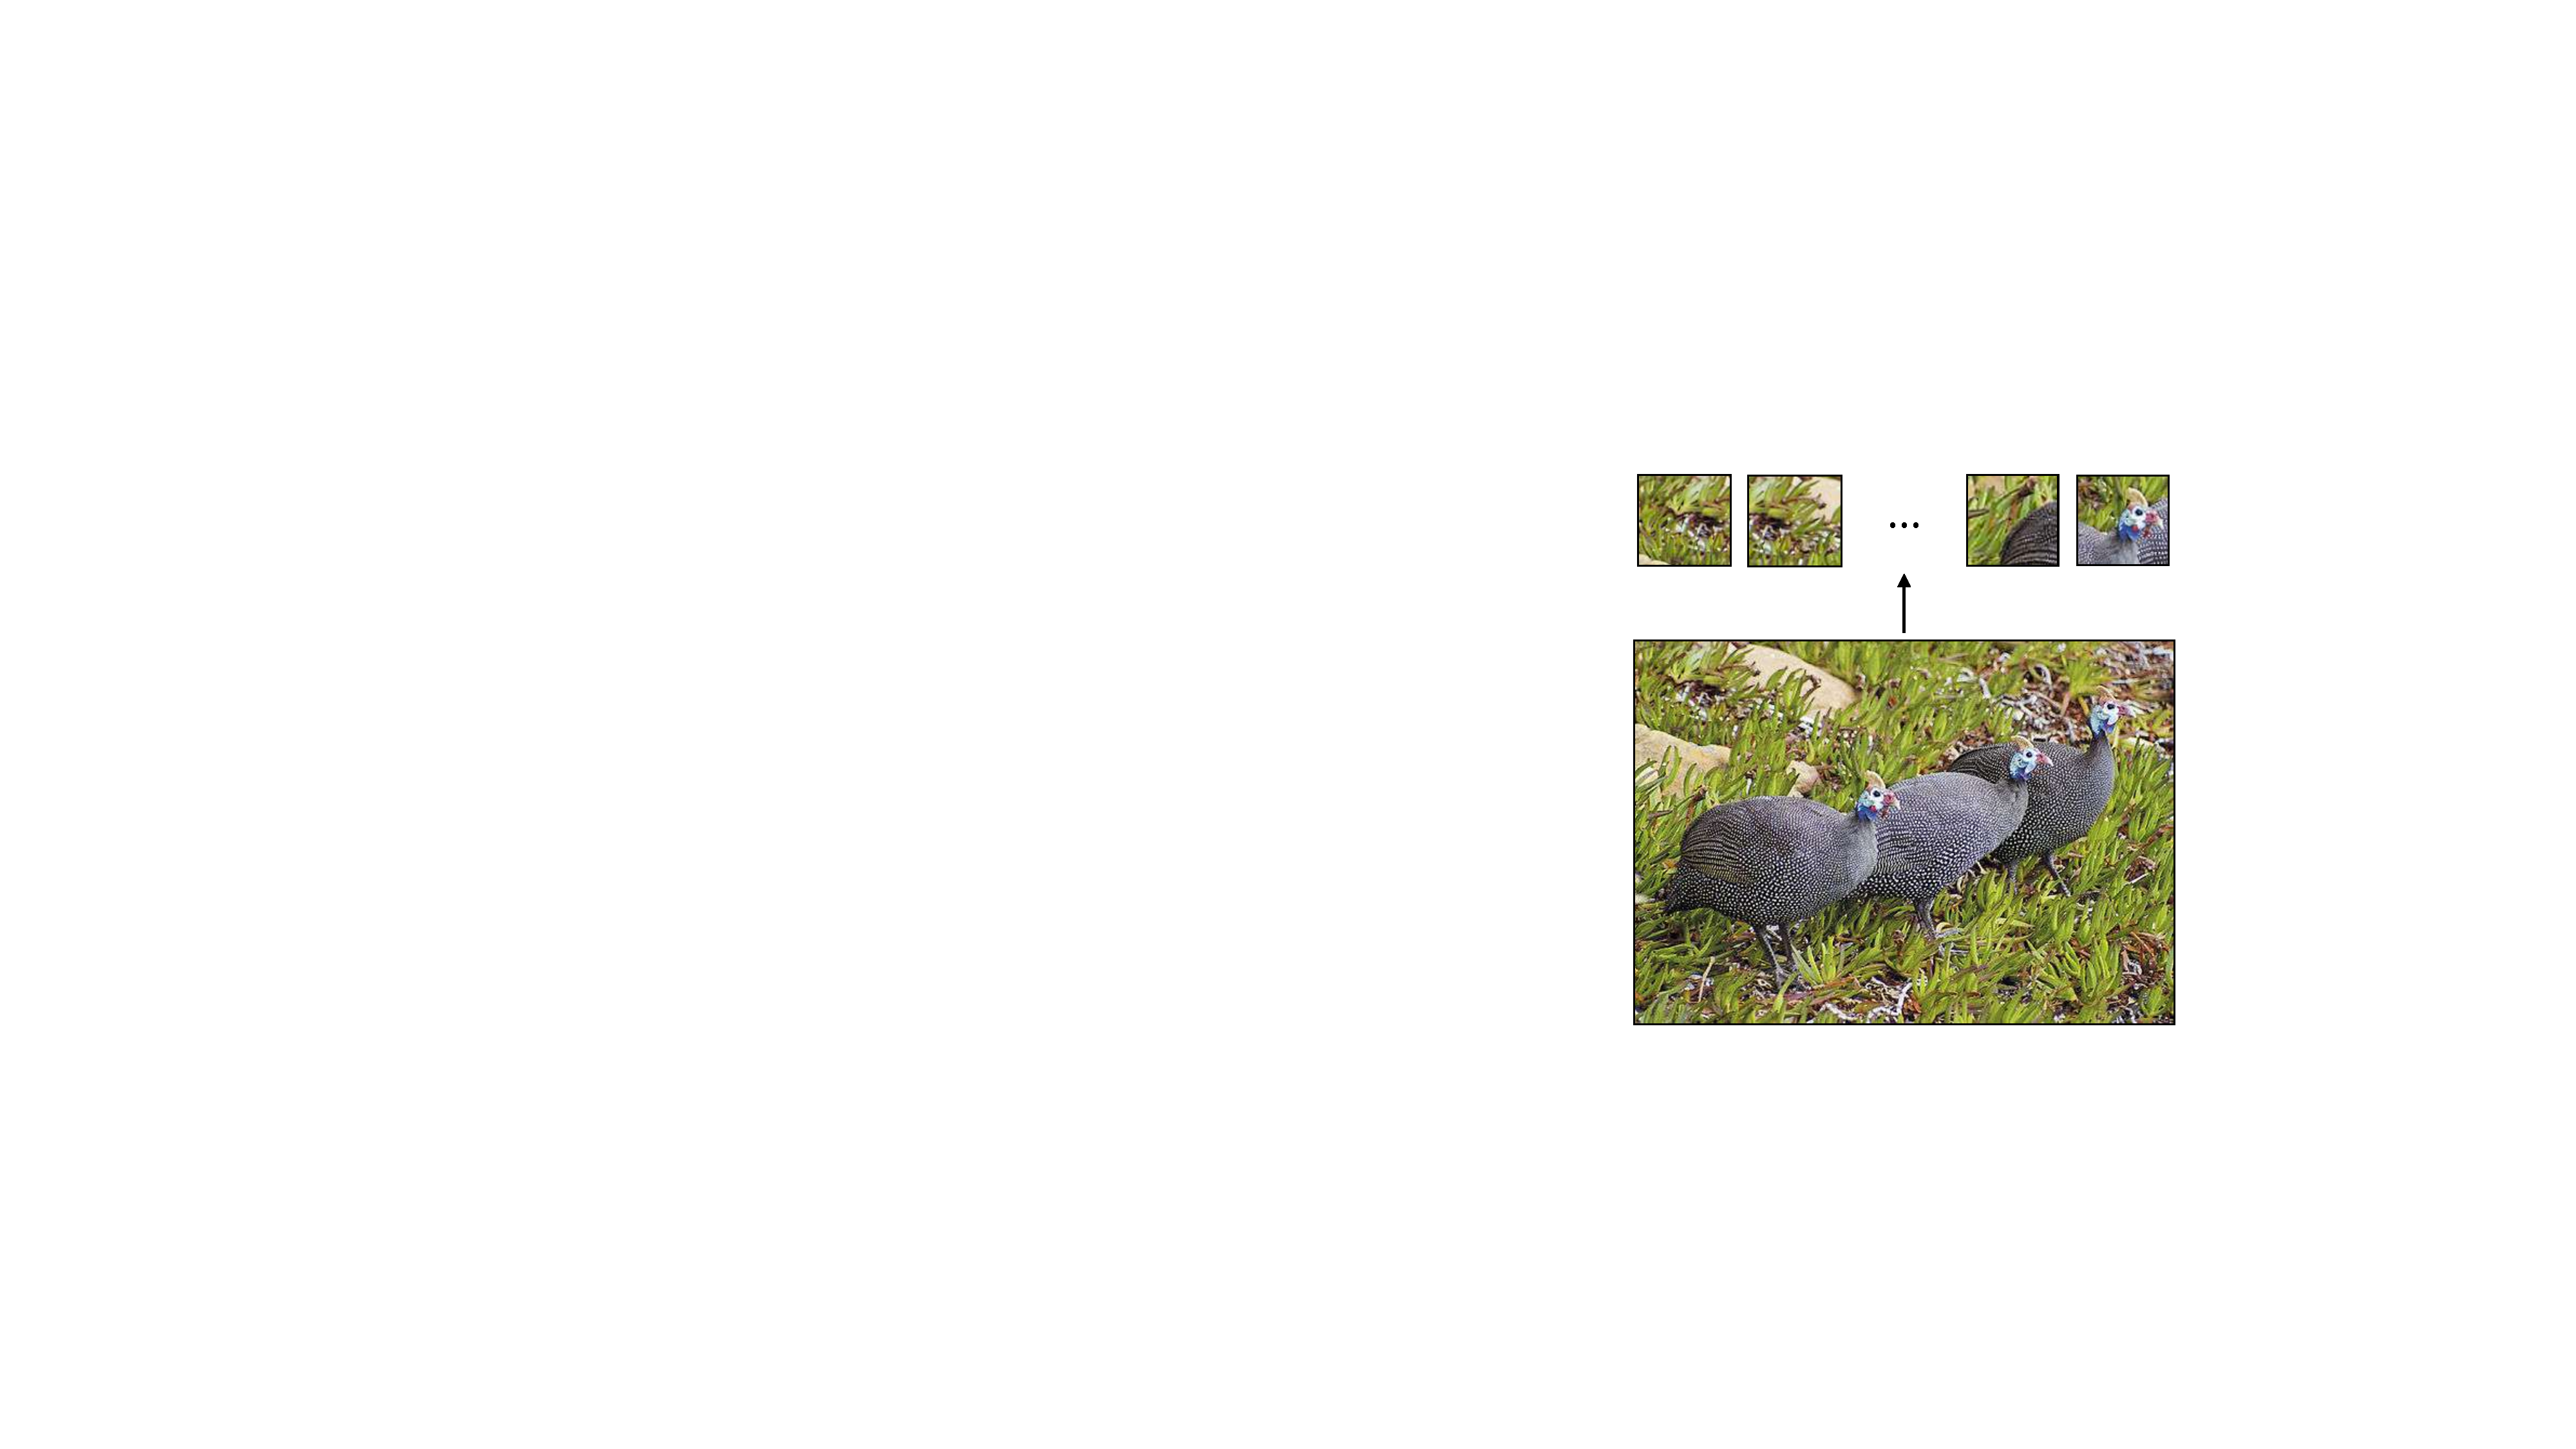
\includegraphics[width=0.31\linewidth]{./figures/transformers/tokenization.pdf}};
%
\def\neuronrad{0.3}
% \draw [fill=white] (-2.075,1.5) rectangle ++(\neuronrad/2,\neuronrad*2);
% \draw [fill=white] (-1.2,1.5) rectangle ++(\neuronrad/2,\neuronrad*2);
% \draw [fill=white] (0.55,1.5) rectangle ++(\neuronrad/2,\neuronrad*2);
% \draw [fill=white] (1.425,1.5) rectangle ++(\neuronrad/2,\neuronrad*2);
\draw [nn_edge, thick] (-1.75,2.25) -- (-1.75,2.75);
\draw [nn_edge, thick] (-0.825,2.25) -- (-0.825,2.75);
\draw [nn_edge, thick] (0.875,2.25) -- (0.875,2.75);
\draw [nn_edge, thick] (1.75,2.25) -- (1.75,2.75);
\draw [fill=white] (-1.825,2.75) rectangle ++(\neuronrad/2,\neuronrad*2);
\draw [fill=white] (-0.95,2.75) rectangle ++(\neuronrad/2,\neuronrad*2);
\draw [fill=white] (0.8,2.75) rectangle ++(\neuronrad/2,\neuronrad*2);
\draw [fill=white] (1.675,2.75) rectangle ++(\neuronrad/2,\neuronrad*2);
%
\draw (-3.3, 3.05) node {tokens}; \draw (-2.5,2.75) -- (-2.5,3.35);
\draw (-3.3, 1.8) node {patches}; \draw (-2.5,1.45) -- (-2.5,2.15);
\draw (-3.3, -0.7) node {input}; \draw (-2.5,-2.2) -- (-2.5,0.8);
\end{tikzpicture}
}
\caption{Tokenization: converting an image to a set of vectors.}
\label{fig:transformers:tokenization}
\end{figure}

%In language modeling, a token might represent a word, so that a sequence of tokens is a sentence. In computer vision, a token may correspond to an image patch, so that an array of tokens represents an image.


\subsection{Mixing tokens}
Once we have converted our data to tokens, we now need to define operations for transforming these tokens and eventually making decisions based on them. The first key operation we will define is how to take \textit{linear combinations of tokens}.

%Let $t_1$, $t_2$, $t_3$ be tokens and $\alpha$, $\beta$ be scalars. $t_1$ is a vector of neurons $[t_1[1], \ldots, t_1[N]]$, and correspondingly for $t_2$ and $t_3$. Then we define summation as:
%\begin{align}
%    t_3 &= t_1 + t_2\\
%        &\equiv [t_1[1],\ldots,t_1[N]] + [t_2[1],\ldots,t_2[N]]\\
%        &\equiv [t_1[1]+t_2[1],\ldots,t_1[N]+t_2[N]]
%\end{align}
%And we define multiplication by a scalar $\alpha$ as:
%\begin{align}
%    t_2 &= \alpha*t_1\\
%        &\equiv \alpha*[t_1[1],\ldots,t_1[N]]\\
%        &\equiv [\alpha*t_1[1],\ldots,\alpha*t_1[N]]
%\end{align}
%This is just what you would expect if a token were considered a vector.

A linear combination of tokens is not the same as a fully connected layer in a neural net. Instead of taking a weighted sum of scalar neurons, it takes a weighted sum of token code vectors: %You can think of this operation as a linear transformation with block structure.
\marginnote{As notational convenience, in this chapter we define $\xin = [x_1, \ldots, x_N]$ and $\tin = [t_1, \ldots, t_N]$.} 
\begin{align}
    %\xoutj &= \sum_i w_{ij} \xini \quad\quad &\triangleleft \quad \text{linear comb of neurons}\\
    %\Xoutj &= \sum_i w_{ij} \Xini \quad\quad &\triangleleft \quad \text{linear comb of tokens}\\
    %\Xoutjk &= \sum_i w_{ij} \Xinik
    x_{\texttt{out}} &= \sum_{i=1}^N w_{i}\xini \quad\quad &\triangleleft \quad \text{linear comb of neurons}\\
    t_{\texttt{out}}.\mathbf{z} &= \sum_{i=1}^N w_{i} \tini.\mathbf{z} \quad\quad &\triangleleft \quad \text{linear comb of tokens} \label{eqn:transformers:lin_comb_tokens}
    %\mathbf{x}_{\texttt{out}} &\equiv \sum_i w_{i} \Xin[:,i] 
\end{align}
\vspace{-15pt}
% Let $a$ and $b$ be two tokens:
% \begin{align}
%     a &= [a_1, \ldots, a_n]\\
%     b &= [b_1, \ldots, b_n]
% \end{align}
% Then we define the $+$ operator over tokens as an elementwise sum:
% \begin{align}
%     a + b \equiv [a_1 + b_1, \ldots, a_n + b_n]
% \end{align}
% Multiplication of a token $a$ with a scalar $w$ is defined as:
% \begin{align}
%     wa \equiv [wa_1, \ldots, wa_n]
% \end{align}
%Here, capital $\mathbf{X}$ is a matrix with each column being a token vector. You can think of $\mathbf{X}$ as being either a vector of tokens (a vector of vectors) or as a matrix of neurons (scalars). In the following sections, we will generally think of $\mathbf{X}$ as a vector, so that token operations become analogous to neural operations, just at a group level.
% \begin{figure}[h]
%     \centering
%     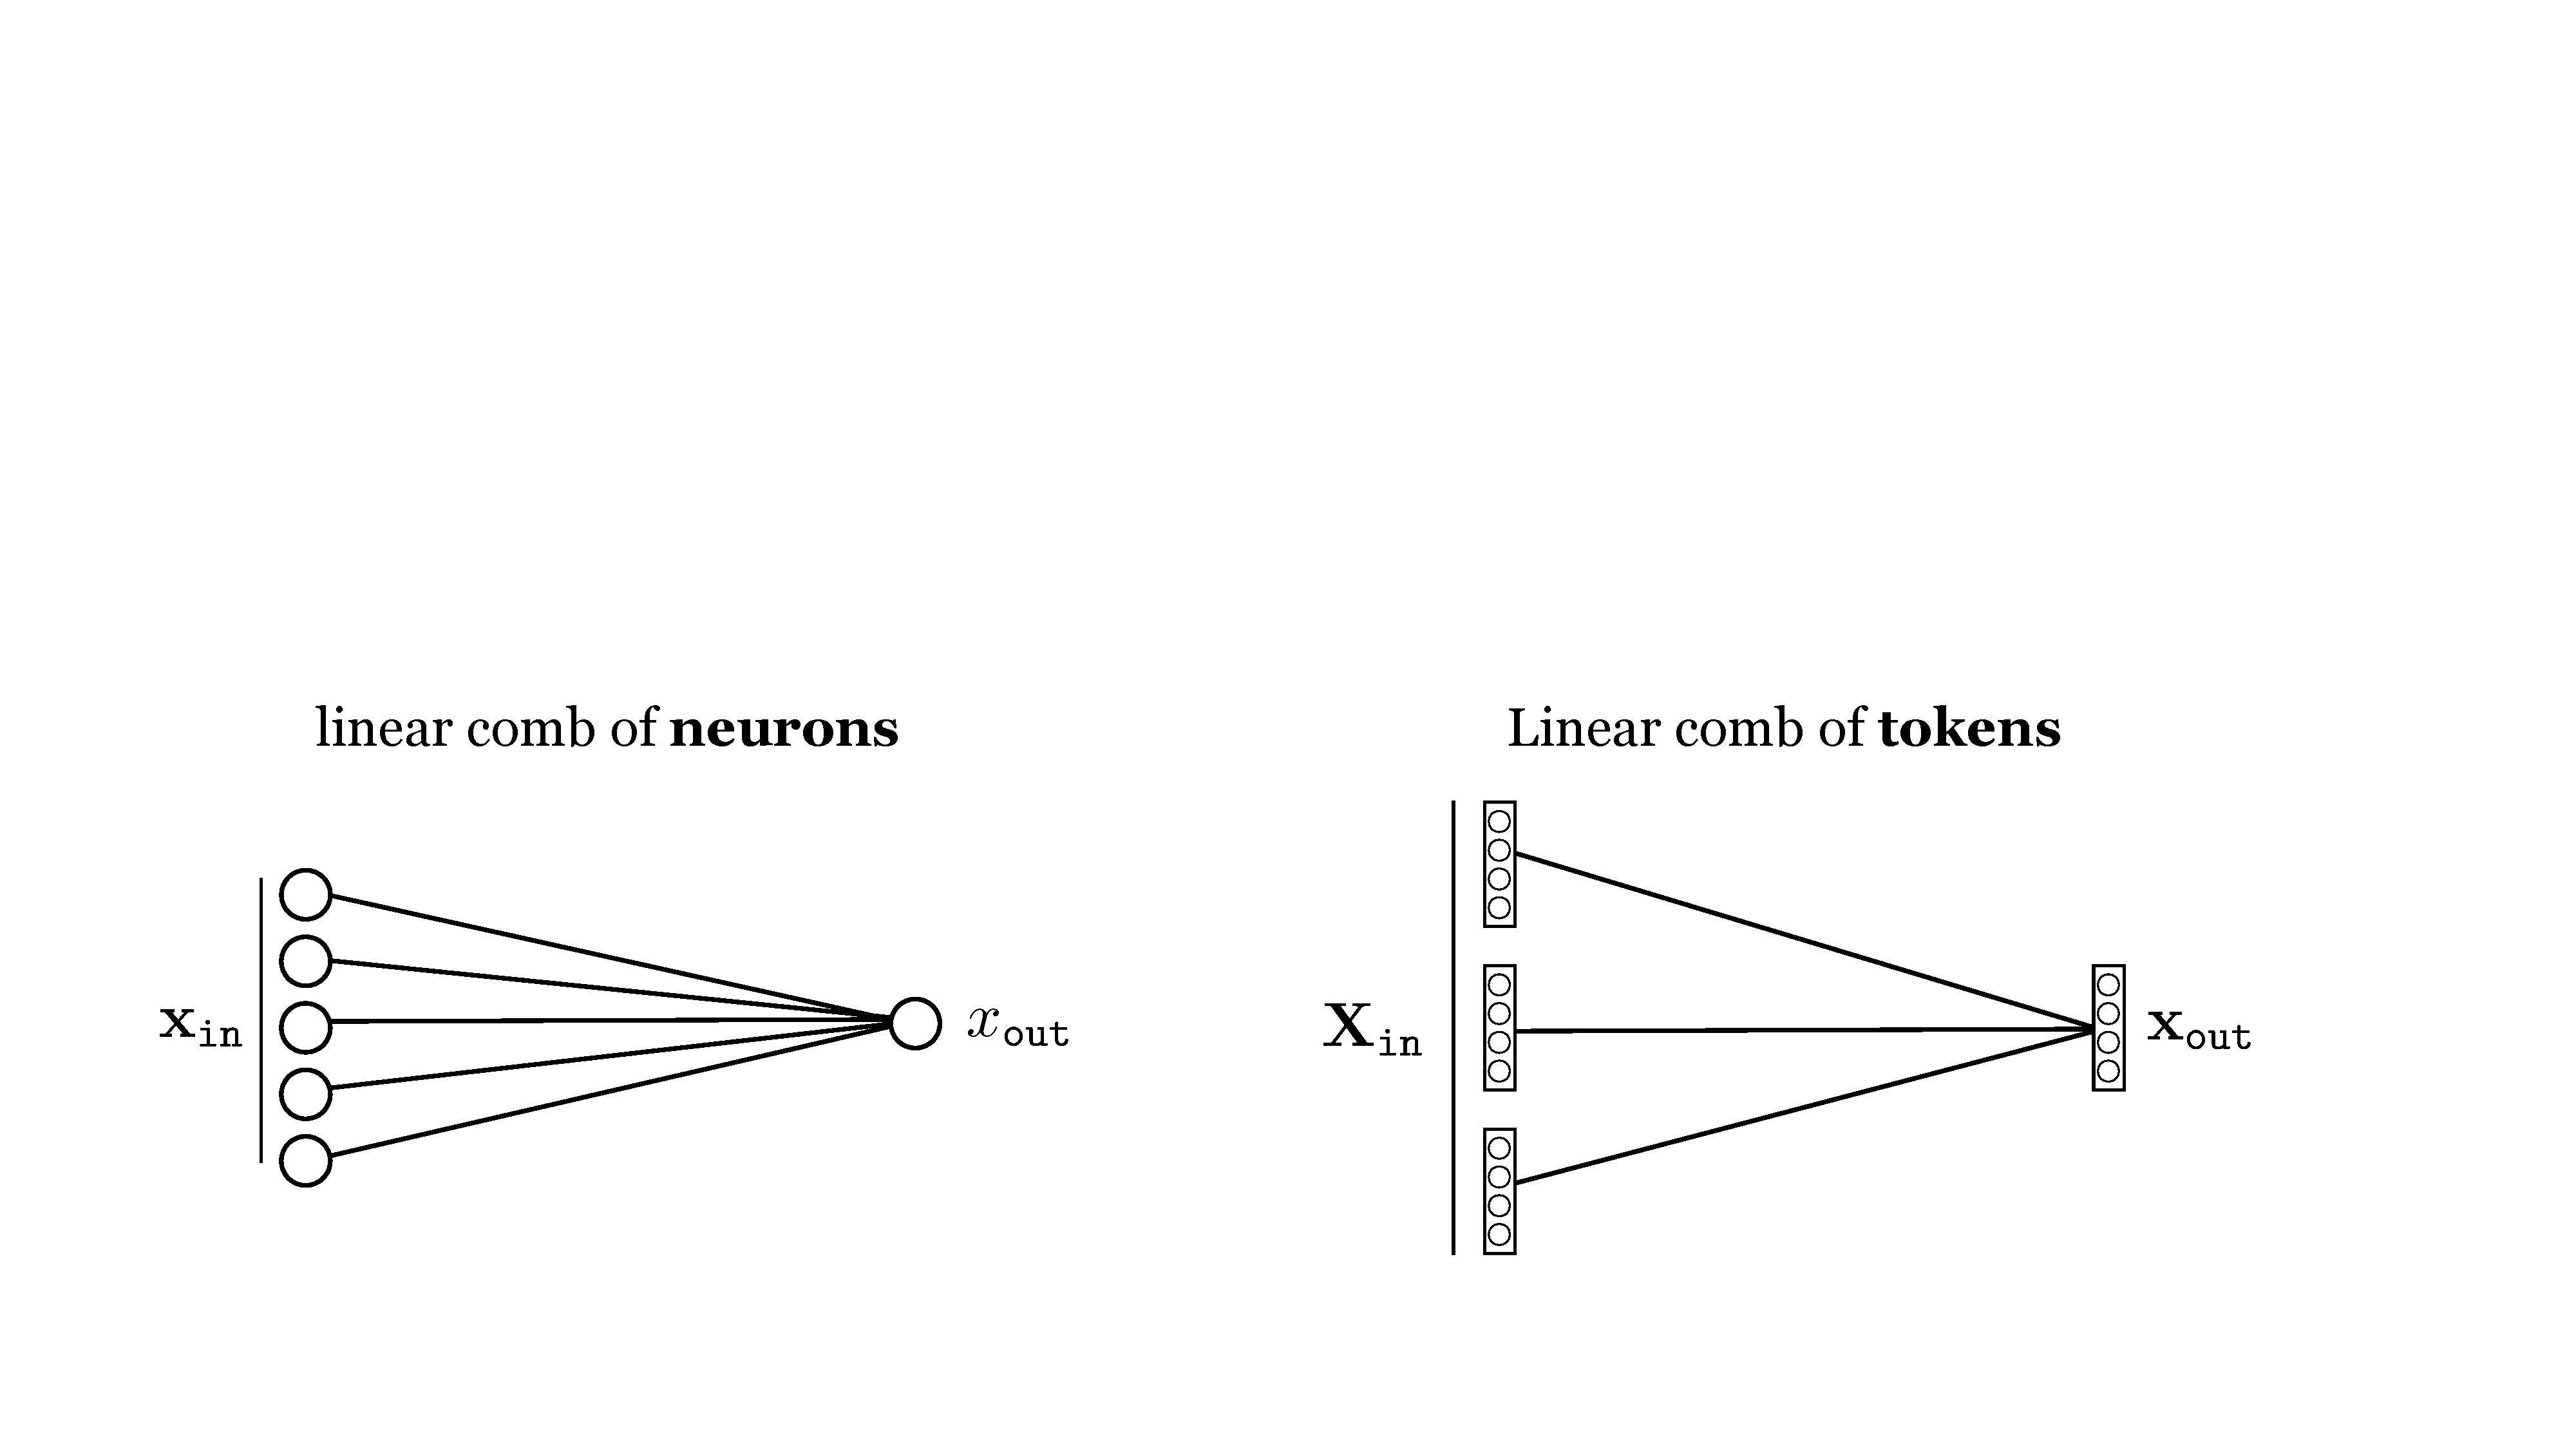
\includegraphics[width=0.9\linewidth]{./figures/transformers/lin_comb_neurons_vs_tokens.pdf}
%     \label{fig:transformers:lin_comb_neurons_vs_tokens}
%     \vspace{-0.4cm}
% \end{figure}
\begin{figure}[h]
\centerline{
\begin{minipage}{.49\linewidth}
\centering
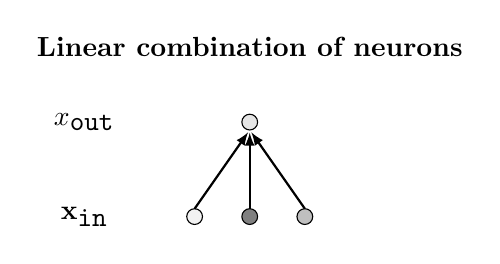
\begin{tikzpicture}
%
\def\Nnodes{3}
\def\layerheight{1.2}
\def\neuronrad{0.1}
\def\neuronstep{0.7}
\draw [fill=gray!10] (\neuronstep,0) circle (\neuronrad);
\draw [fill=gray!100] (\neuronstep*2,0) circle (\neuronrad);
\draw [fill=gray!50] (\neuronstep*3,0) circle (\neuronrad);

\draw [fill=gray!20] (\neuronstep*2,\layerheight) circle (\neuronrad);
\foreach \x in {1,...,\Nnodes} {
    \draw [thick] [nn_edge] (\neuronstep*\x,\neuronrad) -- (\neuronstep*2,\layerheight-\neuronrad);
}
%
\draw (\neuronstep*2,1.8*\layerheight) node {\textbf{Linear combination of neurons}};
\draw (-\neuronstep,0) node {$\xin$};
\draw (-\neuronstep,\layerheight) node {$x_{\texttt{out}}$};
\end{tikzpicture}
\end{minipage}
\begin{minipage}{.49\linewidth}
\centering
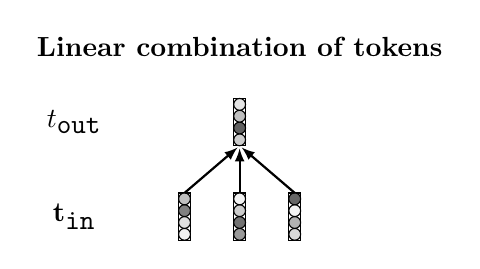
\begin{tikzpicture}
%
\def\Nnodes{3}
\def\layerheight{1.2}
\def\neuronrad{0.3}
\def\neuronstep{0.7}
\foreach \x in {1,...,\Nnodes} {
    \draw (\neuronstep*\x-\neuronrad/4,(0-\neuronrad) rectangle ++(\neuronrad/2,\neuronrad*2);
}
\draw [fill=gray!10] (\neuronstep,\neuronrad*2*0.25-\neuronrad-\neuronrad*0.25) circle (\neuronrad*0.25);
\draw [fill=gray!25] (\neuronstep,\neuronrad*2*0.25*2-\neuronrad-\neuronrad*0.25) circle (\neuronrad*0.25);
\draw [fill=gray!100] (\neuronstep,\neuronrad*2*0.25*3-\neuronrad-\neuronrad*0.25) circle (\neuronrad*0.25);
\draw [fill=gray!50] (\neuronstep,\neuronrad*2*0.25*4-\neuronrad-\neuronrad*0.25) circle (\neuronrad*0.25);

\draw [fill=gray!80] (\neuronstep*2,\neuronrad*2*0.25-\neuronrad-\neuronrad*0.25) circle (\neuronrad*0.25);
\draw [fill=gray!110] (\neuronstep*2,\neuronrad*2*0.25*2-\neuronrad-\neuronrad*0.25) circle (\neuronrad*0.25);
\draw [fill=gray!40] (\neuronstep*2,\neuronrad*2*0.25*3-\neuronrad-\neuronrad*0.25) circle (\neuronrad*0.25);
\draw [fill=gray!10] (\neuronstep*2,\neuronrad*2*0.25*4-\neuronrad-\neuronrad*0.25) circle (\neuronrad*0.25);

\draw [fill=gray!30] (\neuronstep*3,\neuronrad*2*0.25-\neuronrad-\neuronrad*0.25) circle (\neuronrad*0.25);
\draw [fill=gray!60] (\neuronstep*3,\neuronrad*2*0.25*2-\neuronrad-\neuronrad*0.25) circle (\neuronrad*0.25);
\draw [fill=gray!10] (\neuronstep*3,\neuronrad*2*0.25*3-\neuronrad-\neuronrad*0.25) circle (\neuronrad*0.25);
\draw [fill=gray!120] (\neuronstep*3,\neuronrad*2*0.25*4-\neuronrad-\neuronrad*0.25) circle (\neuronrad*0.25);

\draw (\neuronstep*2-\neuronrad/4,(\layerheight-\neuronrad) rectangle ++(\neuronrad/2,\neuronrad*2);

\draw [fill=gray!40] (\neuronstep*2,\layerheight+\neuronrad*2*0.25-\neuronrad-\neuronrad*0.25) circle (\neuronrad*0.25);
\draw [fill=gray!125] (\neuronstep*2,\layerheight+\neuronrad*2*0.25*2-\neuronrad-\neuronrad*0.25) circle (\neuronrad*0.25);
\draw [fill=gray!50] (\neuronstep*2,\layerheight+\neuronrad*2*0.25*3-\neuronrad-\neuronrad*0.25) circle (\neuronrad*0.25);
\draw [fill=gray!20] (\neuronstep*2,\layerheight+\neuronrad*2*0.25*4-\neuronrad-\neuronrad*0.25) circle (\neuronrad*0.25);

\foreach \x in {1,...,\Nnodes} {
    \draw [thick] [nn_edge] (\neuronstep*\x,\neuronrad) -- (\neuronstep*2,\layerheight-\neuronrad);
}
%
\draw (\neuronstep*2,1.8*\layerheight) node {\textbf{Linear combination of tokens}};
\draw (-\neuronstep,0) node {$\tin$};
\draw (-\neuronstep,\layerheight) node {$t_{\texttt{out}}$};
\end{tikzpicture}
\end{minipage}
}
\caption{Linear combination of neurons vs tokens.}
\end{figure}

Operations over tokens can be defined just like operations over neurons except that the tokens are vector-valued while the neurons are scalar-valued. Most layers we have seen can be defined for tokens in an analogous way to how they were defined for neurons, like we saw with the token linear combination. %For example, we can define a $\texttt{relu}$ layer over tokens as:
%\begin{align}
%    \Xout &= \texttt{relu}(\Xin) = [\texttt{relu}(\mathbf{X}_{\texttt{in}_1}), \ldots, \texttt{relu}(\XinN)] \quad\quad &\triangleleft \quad \texttt{relu} \text{ over tokens}
%\end{align}
%In words, we just apply the regular $\texttt{relu}$ operator to each token in the matrix $\mathbf{X}$.
%In words, we just apply $\texttt{relu}$ element-wise to each element of $\Xin$.

For example, we define an fc-layer over token codes as a mapping from $N_1$ input tokens to $N_2$ output tokens, parameterized by a matrix $\mathbf{W} \in \mathbb{R}^{N_2 \times N_1}$ (and, optionally, a set of biases $\mathbf{b} \in \mathbb{R}^{N_2 \times M}$ (for token's with $M$-dimensional code vectors).

For vector-valued tokens, these layers can be written compactly by defining $\Zin \in \mathbb{R}^{N_1 \times M}$ and $\Zout \in \mathbb{R}^{N_2 \times M}$ as matrices whose rows are $M$-dimensional token code vectors (transposed since by convention we use column vectors in this book): 
\begin{equation}
    \Zin = 
     \begin{pmatrix}
        t_1.\mathbf{z}^T\\
        \vdots \\
        t_N.\mathbf{z}^T\\
    \end{pmatrix}
\end{equation}

Then the fc-layer over token codes can be written as:
\begin{align}
    \Zout &= \mathbf{W}\Zin + \mathbf{b} \quad\quad &\triangleleft \quad \text{fc-layer over token codes}
\end{align}
\marginnote{This notation is compact and turns working with tokens into an exercise in matrix algebra. However, the notation here is also somewhat limiting, as it only applies to vector-valued tokens. What if we want tokens that are tensor-valued, or tokens whose codes are elements of an abstract group such as SO(3)? There is not yet standard notation for working with tokens like this. As you read this chapter try to think about how the operations we define for standard vector-valued tokens could be instead defined for other kinds of tokens.}[-3.6cm]

Notice how the structure is analogous to fc-layers over neurons, except that the elements of the input are vector-valued. We can proceed in this fashion and make analogous token layers for any neuron-layer. For example, we could define a convolution layer over tokens as just like a convolution over neurons except that each weighted sum is a linear combination of tokens rather than a linear combination of neurons. Let's write this out for the simple case of 1D convolution with a single filter $\mathbf{w}$ over a 1D array of token code vectors:
\begin{align}
    \tout.\mathbf{z} &= \mathbf{w} \circ \tin.\mathbf{z} \quad\quad &\triangleleft \quad \text{conv over token codes}\\
    \tout[i].\mathbf{z} &= \sum_{k=-N}^N \mathbf{w}[k] \tin[i-k].\mathbf{z}
    %\Xout &= \mathbf{w} \star \Xin\\
    %\Xout[n,:] &\equiv \sum_{k=-N}^N \mathbf{w}[k] \Xin[n-k,:]
\end{align}
% As another example, here is how we define softmax over tokens:
% \begin{align}
%     \xouti &= \frac{e^{-\tau \xini}}{\sum_{k=1}^K e^{-\tau \xink}} \quad\quad &\triangleleft \texttt{softmax over neurons}\\
%     \Xoutij &= \frac{e^{-\tau \Xinij}}{\sum_{k=1}^K e^{-\tau \Xinkj}} \quad\quad &\triangleleft \texttt{softmax over tokens}
% \end{align}
% In other words, we have simply applied the regular softmax function over each column of $\Xin$.
This layer is not currently popular but maybe it will be in the future. For any neural layer you come across, you may want to consider: what if I make it a token layer instead?

\subsection{Modifying tokens}\label{sec:transformers:modifying_tokens}
Linear combinations only let us linearly mix and recombine tokens, and stacking linear functions can only result in another linear function. In standard neural nets, we ran into the same problem with fully-connected and convolutional layers, which, on their own, are incapable of modeling nonlinear functions. To get around this limitation, we added \textit{pointwise nonlinearities} to our neural nets. These are functions that apply a nonlinear transformation to each neuron \textit{individually}, independently from all other neurons. Analogously, for ``token networks" we will also introduce ``pointwise" operators -- these are functions that apply a nonlinear transformation to each token individually, independently from all other tokens. Given a nonlinear function $F_{\theta}: \mathbb{R}^N \rightarrow \mathbb{R}^N$, a token-wise nonlinearity layer can be expressed as:
\begin{align}
    \tout = [F_{\theta}(t_1.\mathbf{z}), \ldots, F_{\theta}(t_N.\mathbf{z})] \quad\quad \triangleleft \text{ per-token nonlinearity}
    %\tout = [F_{\theta}(\mathbf{z}^{t_{\texttt{in}_1}}), \ldots, F_{\theta}(\mathbf{z}^{t_{\texttt{in}_N}})] \quad\quad \triangleleft \text{ per-token nonlinearity}
    %\Xout = [F_{\theta}(\Xin[1,:]), \ldots, F_{\theta}(\Xin[N,:])]
\end{align}
Notice that this operation is generalization of the pointwise nonlinearity in regular neural nets; a $\texttt{relu}$ layer is the special case where $N=1$ and $F_{\theta} = \texttt{relu}$:
\begin{align}
    \xout = [\texttt{relu}(x_1), \ldots,\texttt{relu}(x_N)] \quad\quad \triangleleft \text{ per-neuron nonlinearity (\texttt{relu} layer)}
\end{align}
$F_{\theta}$ may be any nonlinear function but some choices will work better than others. One popular choice is for $F_{\theta}$ to be an MLP (multi-layer perceptron; see chapter \ref{chapter:neural_nets}). In this case, $F_{\theta}$ has learnable parameters $\theta$ which are the weights and biases of the MLP. This reveals an important difference between pointwise operations in regular neural nets and in token nets: $\texttt{relus}$, and most other neuron-wise nonlinearities, have no learnable parameters, whereas $F_{\theta}$ typically does. This is one of the interesting things about working with tokens, the pointwise operations become expressive and parameter-rich.

%So, the ``relus" in token nets are neural nets. The token net is a net of nets.
%Notice that this operation is analogous to the pointwise nonlinearity in neural nets, except that in regular neural nets $F_{\theta}$ is a scalar-to-scalar nonlinearity like a \texttt{relu}, and the operation is over neurons rather than tokens:

%Another  important difference is that in neural nets the pointwise nonlinearity typically has no learnable parameters, whereas when working with tokens we often do learn the parameters of $F_{\theta}$. This is one of the interesting things about working with tokens, the pointwise operations be parameter-rich.

\paragraph*{CNNs in disguise} Pointwise operations apply the same operation independently and identically to all elements of an input array. Where have we seen that before? That's right, convolution! In Chapter \ref{chapter:convolutional_neural_nets} we emphasized that the key idea of CNNs is to break up an input signal into chunks and process each chunk independently and identically.\marginnote{This is such a fundamentally useful idea that it shows up in many different fields under different names. One general name for it is \textbf{factorizing} a problem into smaller pieces.}[-1cm] While a single convolutional layer is linear, a full CNN is a ``pointwise" nonlinear function over patches of the input signal -- and that's precisely what a per-token MLP is, just with patches of spatial size 1x1.

So, for any per-token MLP, there is an equivalent CNN, which only uses kernels of size 1x1. Moreover, the first step in a token-net -- tokenizing the input by vectorizing $k \times k$ patches -- can also be represented as a convolutional layer: in this case there are $N$ filters of size $k \times k$, each of which picks out a single pixel in the image patch, to create $N$ output channels that correspond to the vectorized patch. Really, the only \textit{new} thing in token nets (and transformers, as we will see) is the linear combination of tokens layer (and the attention version of it). Otherwise, transformers are just CNNs in disguise.

As an exercise, we write out below two equivalent views of a per-token MLP, first as a pointwise nonlinearity over tokens and second as a CNN over neurons. The MLP is of the form \texttt{linear}-\texttt{relu}-\texttt{linear}, and the input is a 1D tensor of tokens $\tin$, which can equivalently be represented as a 2D tensor of neurons $\Xin$ whose rows are the token codes:
\begin{align}
    &\tout = [F_{\theta}(t_1.\mathbf{z}), \ldots, F_{\theta}(t_N.\mathbf{z})]
\end{align}
\begin{align}
    &\text{Per-token MLP over $\tin$:}\nonumber \\
    &\quad\quad \mathbf{a} = [\mathbf{W_1}t_1.\mathbf{z} + \mathbf{b}_1, \ldots, \mathbf{W_1}t_N.\mathbf{z} + \mathbf{b}_1] &\quad\quad \triangleleft \quad \texttt{per-token linear}\\
    &\quad\quad \mathbf{h} = [\texttt{relu}(\mathbf{a}_1), \ldots, \texttt{relu}(\mathbf{a}_N)] &\quad\quad \triangleleft \quad \texttt{relu}\\
    &\quad\quad \tout = [\mathbf{W_2}\mathbf{h}_1 + \mathbf{b}_2), \ldots, \mathbf{W_2}\mathbf{h}_N + \mathbf{b}_2] &\quad\quad \triangleleft \quad \texttt{per-token linear}
\end{align}
\begin{align}
    &\text{Equivalent CNN over $\Xin$:}\nonumber \\
    &\quad\quad \mathbf{a}[:,k] = \sum_c \mathbf{W_1}[c,k] \circ \Xin + \mathbf{b}_1[k] \quad \forall k &\quad\quad \triangleleft \quad \texttt{conv}\\
    &\quad\quad \mathbf{h} = [\texttt{relu}(\mathbf{a}[1,:]), \ldots, \texttt{relu}(\mathbf{a}[N,:])] &\quad\quad \triangleleft \quad \texttt{relu}\\
    &\quad\quad \Xout[:,k] = \sum_c \mathbf{W_2}[c,k] \circ \mathbf{h} + \mathbf{b}_2[k] \quad \forall k &\quad\quad \triangleleft \quad \texttt{conv}
\end{align}

\section{Token nets}

We will use the term \textbf{token nets} to refer to computation graphs that use tokens as the primary nodes, rather than neurons.\marginnote{Note that the terminology in this chapter is not standard. The term ``token nets", and the token layer definitions we have given, are our own invention.}[-0.8cm] Token nets are just like neural nets, alternating between layers that mix nodes in linear combinations (e.g., fully-connected linear layers, convolutional layers, etc) and layers that apply a pointwise nonlinearity to each node (e.g., relus, per-token MLPs). Of course, since tokens are simply groups of neurons, every token net is itself also a neural net, just viewed differently -- it is a net of sub-nets. Below we show a standard neural net and a token net side by side, to emphasize the similarities in their operations:

\begin{figure}[h]
\centerline{
\begin{minipage}{.49\linewidth}
\centering
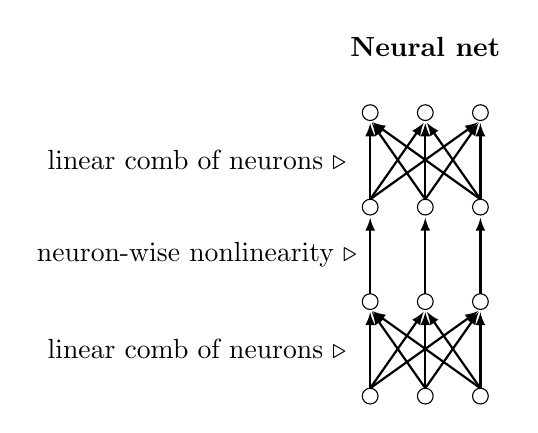
\begin{tikzpicture}
%
\def\Nnodes{3}
\def\Nlayers{4}
\def\layerheight{1.2}
\def\neuronrad{0.1}
\def\neuronstep{0.7}
\foreach \x in {1,...,\Nnodes} {
    \foreach \y in {1,...,\Nlayers} {
        \draw (\neuronstep*\x,(\layerheight*\y-\layerheight) circle (\neuronrad);
    }
}
% mixing layer 1
\foreach \xi in {1,...,\Nnodes} {
    \foreach \xj in {1,...,\Nnodes} {
        \draw [thick] [nn_edge] (\neuronstep*\xi,\neuronrad) -- (\neuronstep*\xj,\layerheight-\neuronrad);
    }
}
% pointwise nonlinearity
\foreach \x in {1,...,\Nnodes} {
    \draw [thick] [nn_edge] (\neuronstep*\x,\layerheight+\neuronrad) -- (\neuronstep*\x,\layerheight*2-\neuronrad);
}
% mixing layer 2
\foreach \xi in {1,...,\Nnodes} {
    \foreach \xj in {1,...,\Nnodes} {
        \draw [thick] [nn_edge] (\neuronstep*\xi,\layerheight*2+\neuronrad) -- (\neuronstep*\xj,\layerheight*3-\neuronrad);
    }
}
%
\draw (\neuronstep*2,3.7*\layerheight) node {\textbf{Neural net}};
\draw (-1.5,0.5*\layerheight) node {linear comb of neurons $\triangleright$};
\draw (-1.5,1.5*\layerheight) node {neuron-wise nonlinearity $\triangleright$};
\draw (-1.5,2.5*\layerheight) node {linear comb of neurons $\triangleright$};
\end{tikzpicture}
\end{minipage}
\begin{minipage}{.49\linewidth}
\centering
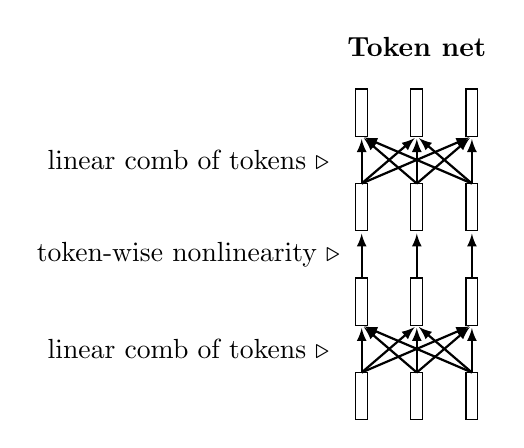
\begin{tikzpicture}
%
\def\Nnodes{3}
\def\Nlayers{4}
\def\layerheight{1.2}
\def\neuronrad{0.3}
\def\neuronstep{0.7}
\foreach \x in {1,...,\Nnodes} {
    \foreach \y in {1,...,\Nlayers} {
        \draw (\neuronstep*\x-\neuronrad/4,(\layerheight*\y-\layerheight-\neuronrad) rectangle ++(\neuronrad/2,\neuronrad*2);
    }
}
% mixing layer 1
\foreach \xi in {1,...,\Nnodes} {
    \foreach \xj in {1,...,\Nnodes} {
        \draw [thick] [nn_edge] (\neuronstep*\xi,\neuronrad) -- (\neuronstep*\xj,\layerheight-\neuronrad);
    }
}
% pointwise nonlinearity
\foreach \x in {1,...,\Nnodes} {
    \draw [thick] [nn_edge] (\neuronstep*\x,\layerheight+\neuronrad) -- (\neuronstep*\x,\layerheight*2-\neuronrad);
}
% mixing layer 2
\foreach \xi in {1,...,\Nnodes} {
    \foreach \xj in {1,...,\Nnodes} {
        \draw [thick] [nn_edge] (\neuronstep*\xi,\layerheight*2+\neuronrad) -- (\neuronstep*\xj,\layerheight*3-\neuronrad);
    }
}
%
\draw (\neuronstep*2,3.7*\layerheight) node {\textbf{Token net}};
\draw (-1.5,0.5*\layerheight) node {linear comb of tokens $\triangleright$};
\draw (-1.5,1.5*\layerheight) node {token-wise nonlinearity $\triangleright$};
\draw (-1.5,2.5*\layerheight) node {linear comb of tokens $\triangleright$};
\end{tikzpicture}
\end{minipage}
}
\caption{Neural nets vs token nets.}
\end{figure}

The arrows here represent any functional dependency between the nodes (note that different arrows represent different types of functions).

% \begin{figure}[h]
%     \centering
%     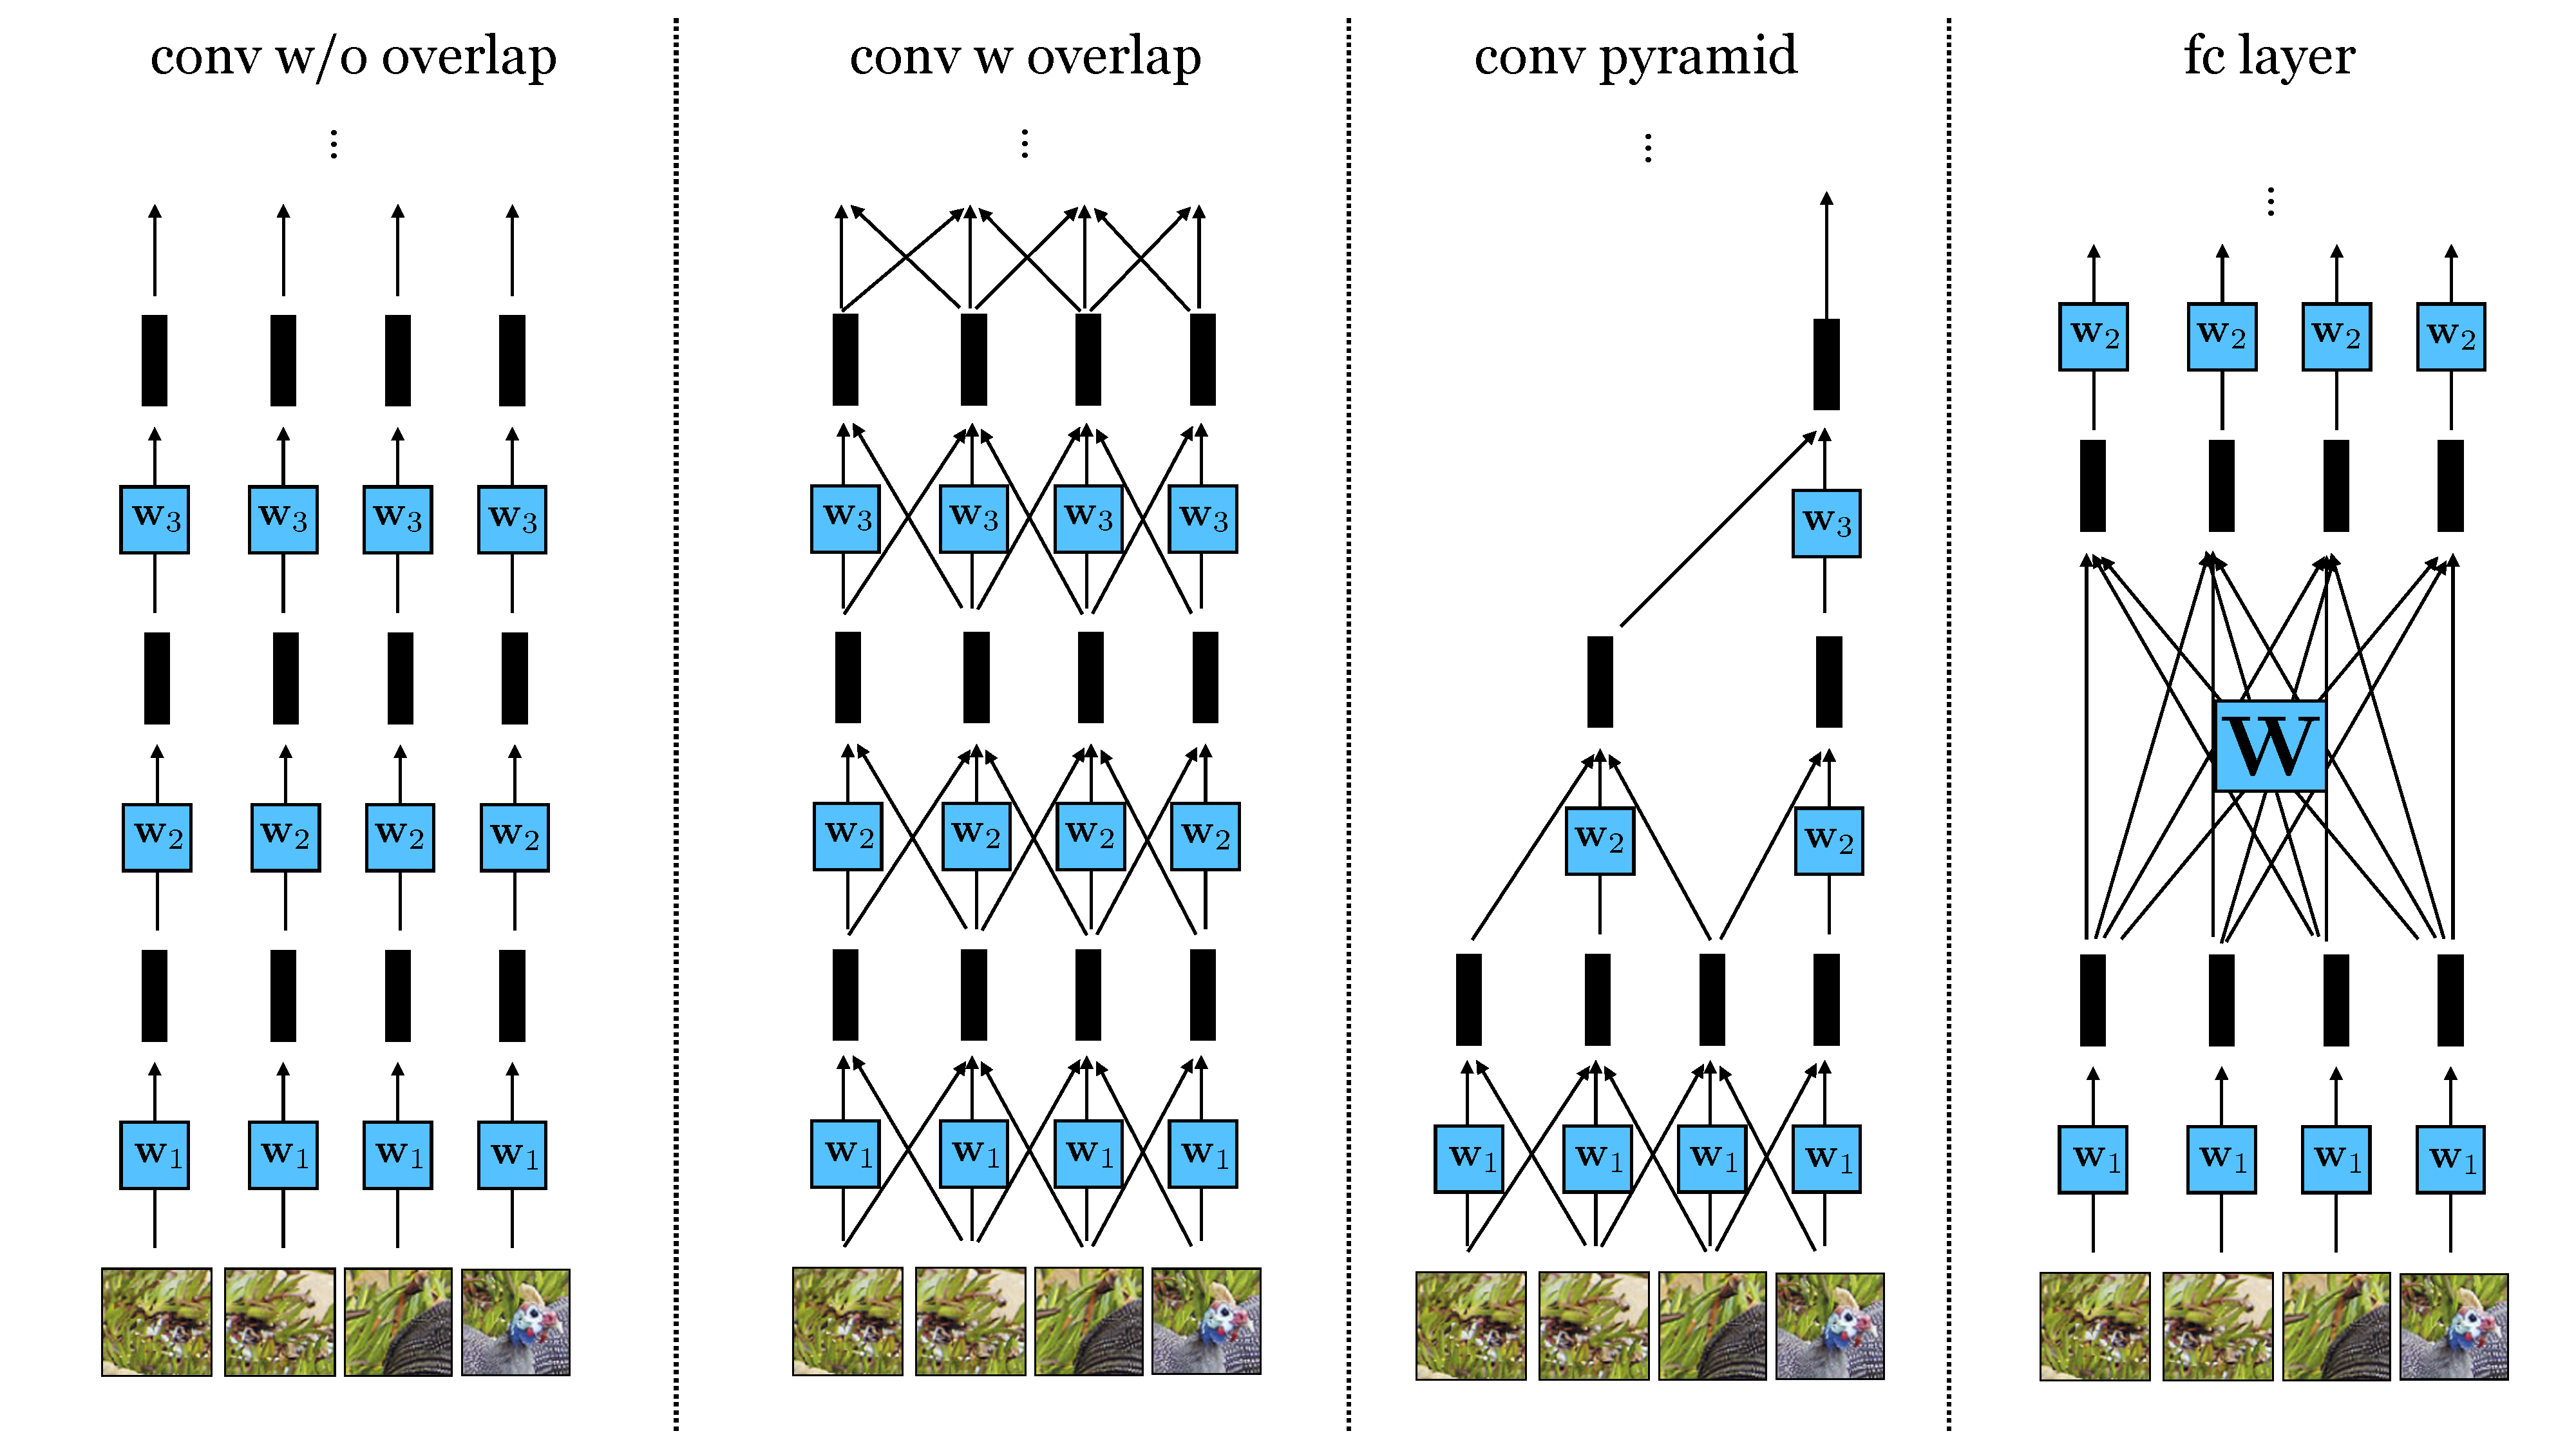
\includegraphics[width=1.0\linewidth]{./figures/transformers/token_mixing_strats.pdf}
% \end{figure}

\section{The attention layer}
\textbf{Attention layers} define a special kind of linear combination of tokens. Rather than parameterizing the linear combination with a matrix of free parameters $\mathbf{W}$, attention layers use a different matrix, which we call the attention matrix $\mathbf{A}$. The important difference between $\mathbf{A}$ and $\mathbf{W}$ is that $\mathbf{A}$ is \textit{data-dependent}, that is, the values of $\mathbf{A}$ are a function the data input to the network. In the diagram below, we indicate the data-dependency with the function labeled $f$, and we color the attention matrix red to indicate that it is constructed from \textit{transformed data} rather than being free parameters (for which we use the color blue):\marginnote{Here, we describe attention as fc layers with data-dependent weights. We could have instead described attention as a kind of \textit{dynanmic pooling}: it's mean pooling but with a weighted average where the weights are dynamically decided based on the input data.}[-3.5cm]
\begin{figure}[h]
\centerline{
\begin{minipage}{.3\linewidth}
\centering
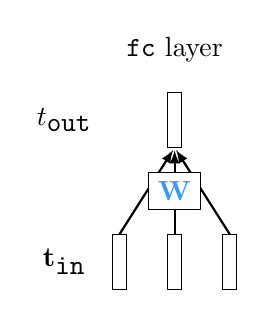
\begin{tikzpicture}
%
\def\Nnodes{3}
\def\Nlayers{2}
\def\layerheight{1.8}
\def\neuronrad{0.35}
\def\neuronstep{0.7}
\foreach \x in {1,...,\Nnodes} {
    \draw (\neuronstep*\x-\neuronrad/4,(\layerheight-\layerheight-\neuronrad) rectangle ++(\neuronrad/2,\neuronrad*2);
}
\draw (\neuronstep*2-\neuronrad/4,(\layerheight*2-\layerheight-\neuronrad) rectangle ++(\neuronrad/2,\neuronrad*2);

% mixing layer 1
\foreach \xi in {1,...,\Nnodes} {
    \draw [thick] [nn_edge] (\neuronstep*\xi,\neuronrad) -- (\neuronstep*2,\layerheight-\neuronrad);
}
%
\draw (0,0) node {$\tin$};
\draw (0,1.8) node {$t_\texttt{out}$};
\draw (1.4,0.5*\layerheight) node[draw,rectangle,fill=white] {$\color{param_color}\mathbf{W}$};
%\draw (3.15,.5*\layerheight) node {$\Longrightarrow$};
\draw (1.4,1.5*\layerheight) node {\texttt{fc} layer};
\end{tikzpicture}
\end{minipage}
\begin{minipage}{.24\linewidth}
\centering
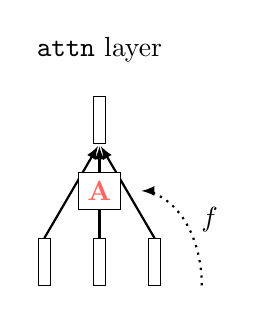
\begin{tikzpicture}
%
\def\Nnodes{3}
\def\Nlayers{2}
\def\layerheight{1.8}
\def\neuronrad{0.3}
\def\neuronstep{0.7}
\foreach \x in {1,...,\Nnodes} {
    \draw (\neuronstep*\x-\neuronrad/4,(\layerheight-\layerheight-\neuronrad) rectangle ++(\neuronrad/2,\neuronrad*2);
}
\draw (\neuronstep*2-\neuronrad/4,(\layerheight*2-\layerheight-\neuronrad) rectangle ++(\neuronrad/2,\neuronrad*2);
% mixing layer 1
\foreach \xi in {1,...,\Nnodes} {
    \draw [thick] [nn_edge] (\neuronstep*\xi,\neuronrad) -- (\neuronstep*2,\layerheight-\neuronrad);
}
%
\draw (1.4,0.5*\layerheight) node[draw,rectangle,fill=white] {$\color{data_color}\mathbf{A}$};
%\draw (2.4, 0.5*\layerheight) node {$\Bigg\}$};
%\draw [thick] [nn_edge] (2.5,0)  .. controls (2.7,0.25*\layerheight) .. (2.0,0.5*\layerheight);
\draw [thick,dotted] [nn_edge] (2.7,-\neuronrad) arc
    [
        start angle=0,
        end angle=90.1,
        x radius=0.8cm,
        y radius=1.2cm
    ];
\draw (2.8,0.3*\layerheight) node {$f$};
\draw (1.4,1.5*\layerheight) node {\texttt{attn} layer};
\end{tikzpicture}
\end{minipage}
}
\caption{Fully-connected layers vs attention layers.}
\end{figure}

The equation for an attention layer is the same as for a linear layer except that the weights are a function of some other data (left unspecified for now but we will see concrete examples below):
\begin{align}
    \mathbf{A} &= f(\ldots) \quad\quad \triangleleft \text{ attention}\\
    \Zout &= \mathbf{A}\Zin
\end{align}

The key question, of course, is ``what exactly is $f$"? What inputs does $f$ depend on and what is $f$'s mathematical form? Before writing out the exact equations, we will start with the intuition: $f$ is a function that determines how much ``attention" to apply to each token in $\tin$; since this layer is just a weighted combination of tokens $f$ is simply determining the weights in this combination. $f$ can depend on any number of input signals that tell the net what to pay attention to.%$f$ is a function that makes it so each token gets to ``attend" over the input data to decide how to update its representation.

As a concrete example, consider that we want to be able to ask questions about different objects in an image, such as ``what color is the bird's head?" Then we can use attention to direct the model to focus on just the object in question -- the bird's head in this example. $f$ would take as input the text query, and would produce as output weights $\mathbf{A}$ that are high for the $\tin$ tokens that correspond to any bird head's and are low for all other $\tin$ tokens. If we train such as system to answer questions about color, then the token codes might end up representing the color of the object in their receptive field; after all, this would be a solution that would solve our problem (it would minimize the loss and correctly answer the question). Other solutions might be possible, but we will focus on this intuitive solution.

What's neat here is that attention gives us a way to make the layer dynamically change its behavior in response to different input questions; asking different questions results in different answers:
\begin{figure}[h!]
\centerline{
\begin{tikzpicture}
    \draw (0, 0) node[inner sep=0] {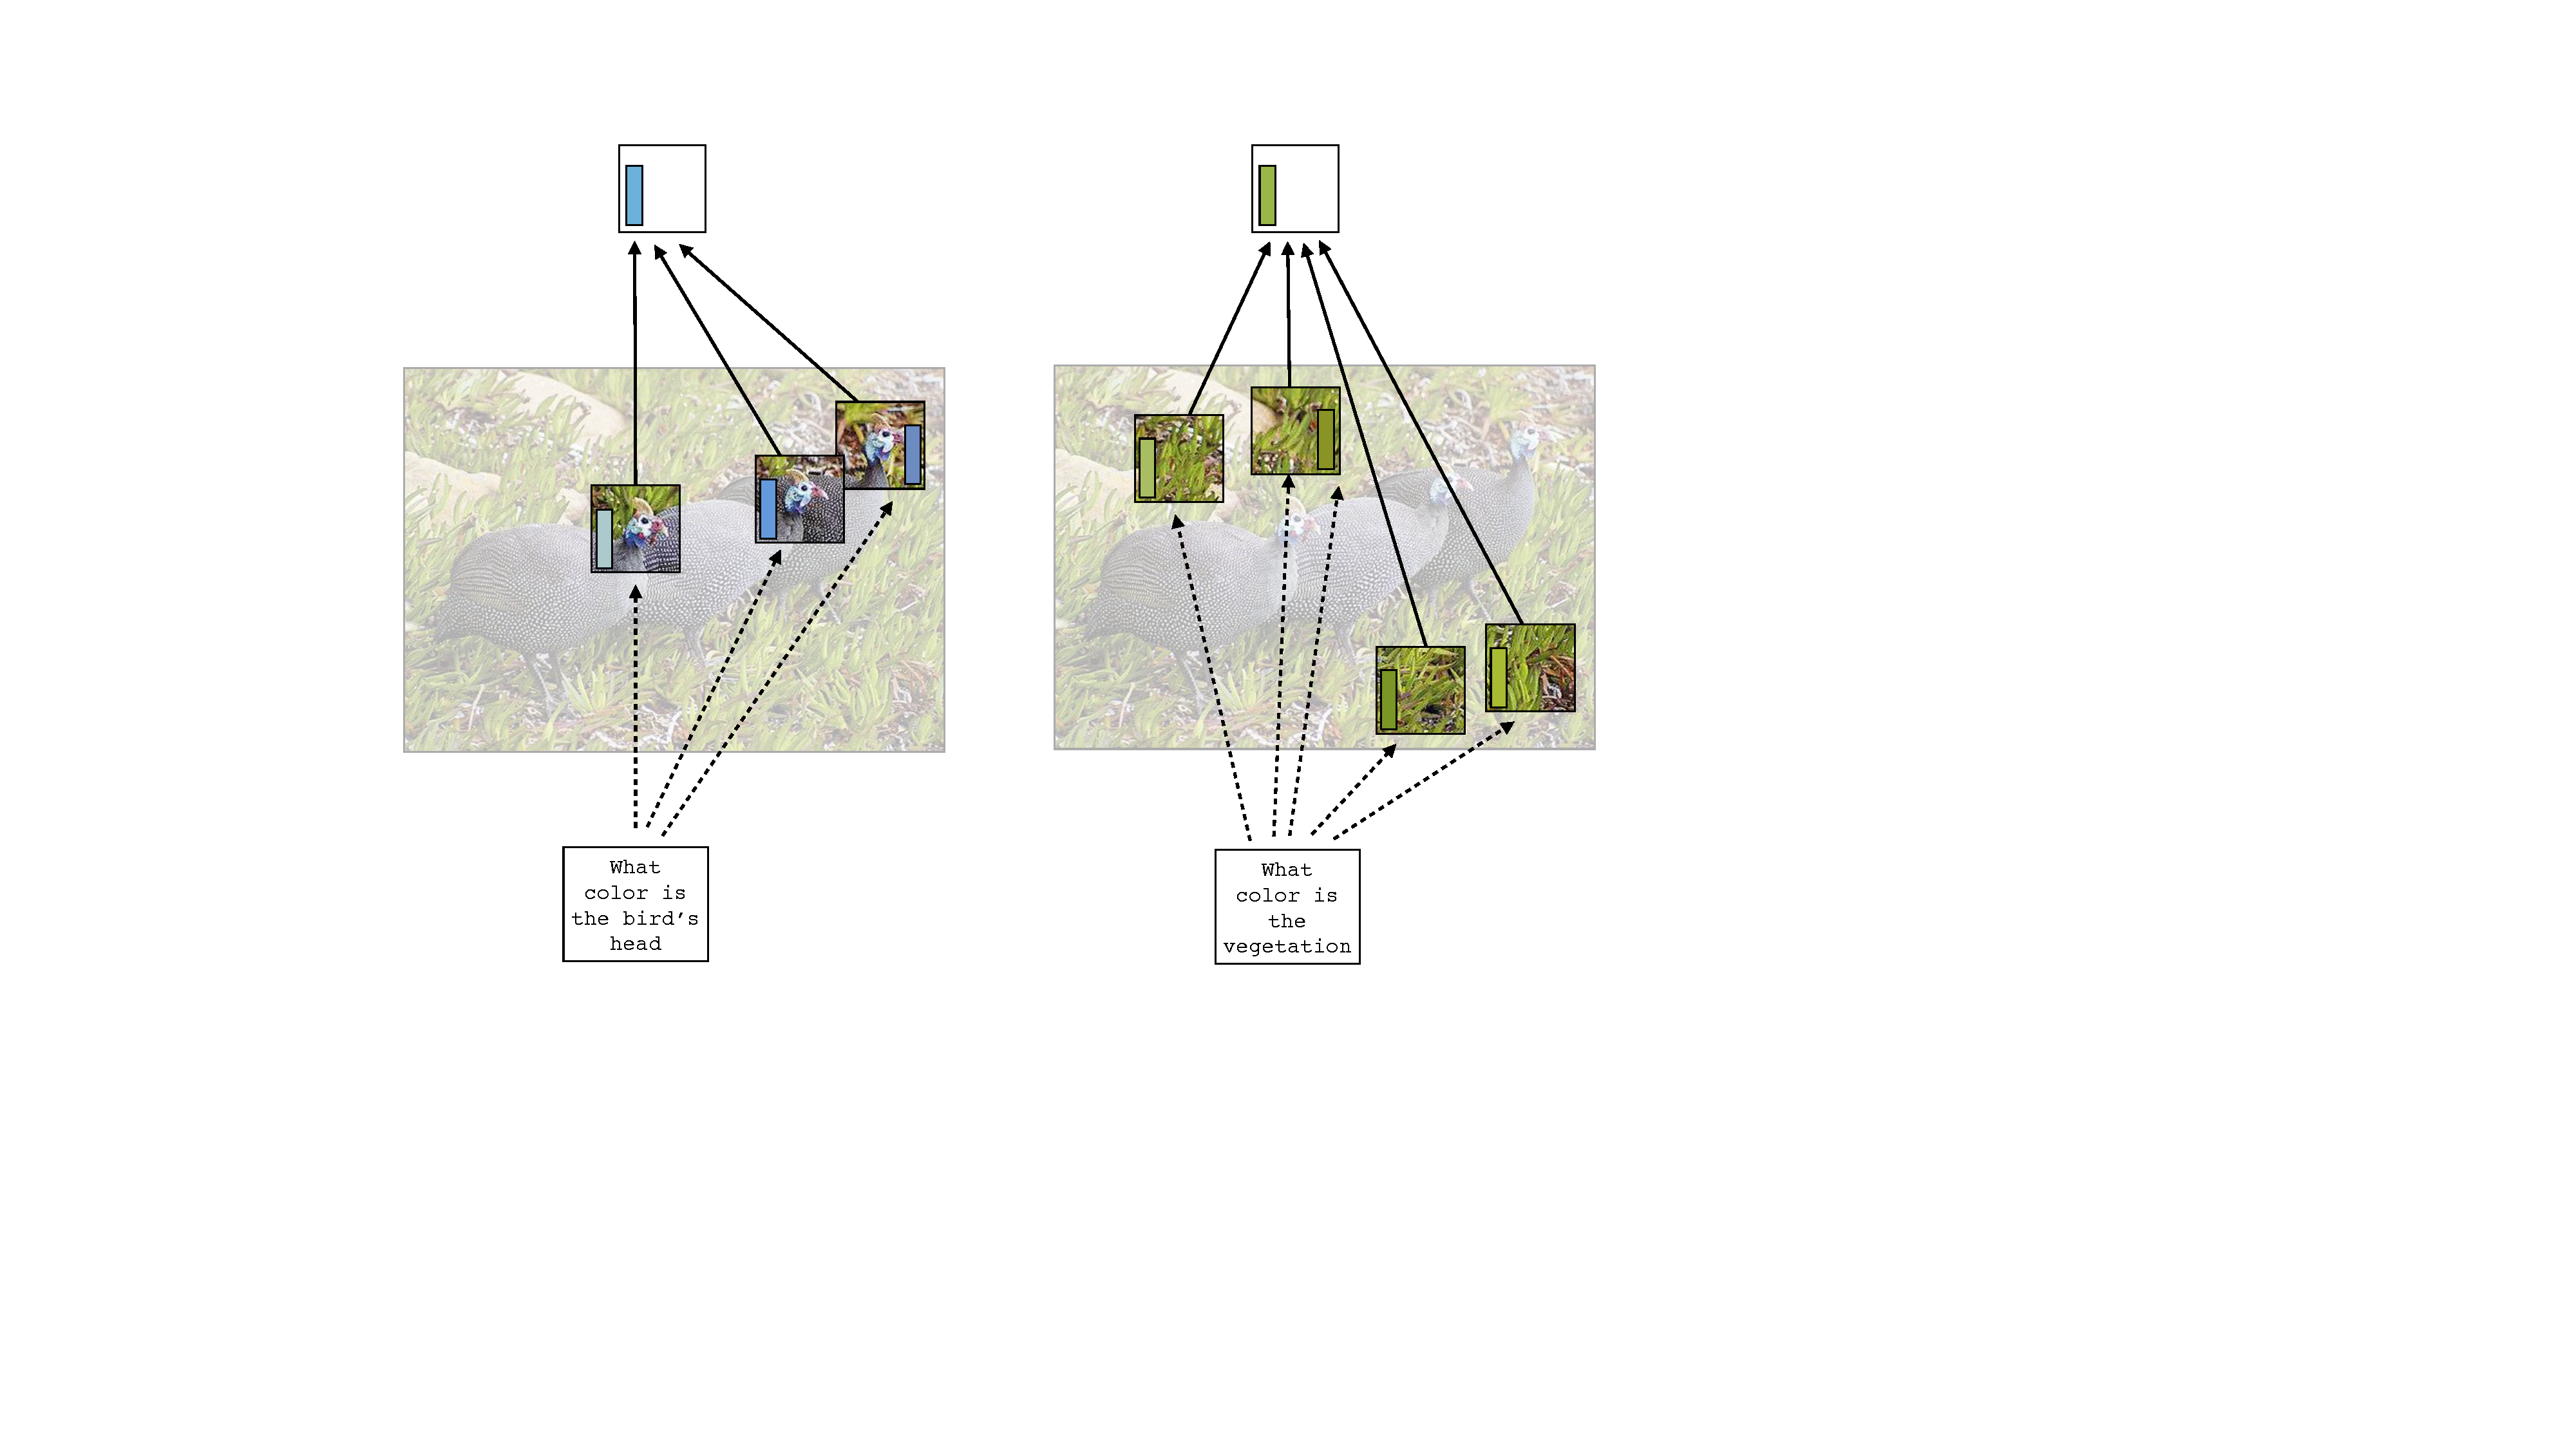
\includegraphics[width=0.9\linewidth]{./figures/transformers/attention_layer_color_query_cartoon.pdf}};
    % \draw (-4.9, 0.9) node [draw,rectangle,fill=white] {$t_{\texttt{in}_3}$};
    % \draw (-2.9, 1.25) node [draw,rectangle,fill=white] {$t_{\texttt{in}_6}$};
    % \draw (-1.9, 1.85) node [draw,rectangle,fill=white] {$t_{\texttt{in}_8}$};
    % \draw (-4.55, 4.9) node [draw,rectangle,fill=white] {$t_\texttt{out}$};
    % %
    % \draw (2, 0.6) node [draw,rectangle,fill=white] {$t_{\texttt{in}_2}$};
    % \draw (2, 1) node [draw,rectangle,fill=white] {$t_{\texttt{in}_3}$};
    % \draw (2, 1.5) node [draw,rectangle,fill=white] {$t_{\texttt{in}_8}$};
    % \draw (2, 1.5) node [draw,rectangle,fill=white] {$t_{\texttt{in}_9}$};
    % \draw (2, 4) node [draw,rectangle,fill=white] {$t_\texttt{out}$};
    %\draw (-6, 4.25) node {$t_\texttt{out}$}; \draw (-5, 4.25) node {$\rightarrow$};
    %\draw (-6, 1.0) node {$\tin$}; \draw (-5.25, 1.0) node {$\Bigg\{$};
    \draw (-6.7, 0) node {$\tin$}; \draw (-6.2,-2) -- (-6.2,2);
    \draw (-6.7, 3.5) node {$t_\texttt{out}$}; \draw (-6.2,3.0) -- (-6.2,4.0);
    \draw (-1.45,-1.55) node {\texttt{attention}};
    \draw (-2.25, 2.75) node {\texttt{sum}};
    \label{fig:attention_layer_color_query_cartoon}
\end{tikzpicture}
}
\caption{How attention can be allocated across different regions (tokens) in an image. The token codes are indicated as the colored rectangles within each token. $t_\texttt{out}$ is a weighted sum over tokens in $\tin$, weighted by attention. Only the tokens that contribute most to this sum are visualized here. On the left, the tokens corresponding to the birds' heads are attended to, whereas on the right, tokens in the background are attended to.}
\end{figure}

Keeping this intuitive picture in mind, we will now turn to the equations that define $f$. We will focus on the particular version of $f$ that appears in transformers, which is called \textbf{query-key-value attention}.

\subsection{Query-Key-Value attention}
Transformers use a particular kind of attention based on the idea of keys, queries, and values.\marginnote{The idea of keys, queries, values comes from databases, where a database cell holds a \textit{value}, which is retrieved when a \textit{query} matches the cell's \textit{key}. Tokens are like database cells and attention is like retrieving information from the database of tokens.}[-1.2cm] In query-key-value attention, each token is associated with a \textbf{query} vector, a \textbf{key} vector, and a \textbf{value} vector. Just like the token's code vector, we can think of these vectors as additional members of the structure $t$. We define these vectors as linear transformations of the token's code vector.\marginnote{Question to think about: could you use other differentiable functions for $\texttt{query}()$, $\texttt{key}()$, and $\texttt{value}()$? Would that be useful?}[2cm] For a token with code vector $\mathbf{z}$, we have:
\begin{align}
    \mathbf{q} &= t.\texttt{query}() = \mathbf{W}_q \mathbf{z} \quad\quad \triangleleft \text{ query}\\
    \mathbf{k} &= t.\texttt{key}() = \mathbf{W}_k \mathbf{z} \quad\quad \triangleleft \text{ key}\\
    \mathbf{v} &= t.\texttt{value}() = \mathbf{W}_v \mathbf{z} \quad\quad \triangleleft \text{ value}
\end{align}

The queries, keys, and values of $\tin$ can compactly be written as matrices:
\begin{equation}
    \Qin = 
     \begin{pmatrix}
        \mathbf{q}_1^T\\
        \vdots \\
        \mathbf{q}_N^T\\
    \end{pmatrix}
    \quad
    \Kin = 
     \begin{pmatrix}
        \mathbf{k}_1^T\\
        \vdots \\
        \mathbf{k}_N^T\\
    \end{pmatrix}
    \quad
    \Vin = 
     \begin{pmatrix}
        \mathbf{v}_1^T\\
        \vdots \\
        \mathbf{v}_N^T\\
    \end{pmatrix}
\end{equation}

In transformers, all inputs to the net are tokenized, so the textual question ``What color is the bird's head" will also be represented as a token.\marginnote{We do not cover them in this book, but methods from natural language processing can be used to transform text into a token, or a sequence of tokens.}[-0.4cm] This token will submit its query vector, $\mathbf{q}_{\texttt{question}}$ to be matched against the keys of the tokens that represent different patches in the image; the similarity between the query and the key determines the amount of attention weight that query will apply to the token with that key. The most common measure of similarity between a query $\mathbf{q}$ and a key $\mathbf{v}$ is the dot product $\mathbf{q}^T\mathbf{v}$. Querying each token in $\tin$ in this way gives us a vector of similarities. We then normalize this vector using the softmax function to give us our attention weights $\mathbf{A}$, and finally, rather than applying $\mathbf{A}$ over token codes directly (i.e. taking a weighted sum over tokens), we take a weighted sum over token values to obtain $\Zout$: %(note that here $\mathbf{A} \in \mathbb{R}^{1 \times N}$ because we only have one output token; later we will see a case where $\mathbf{A} \in \mathbb{R}^{N \times N}$):
\begin{align}
    \mathbf{s} &= [\mathbf{q}_{\texttt{question}}^T\mathbf{k}_1, \ldots, \mathbf{q}_{\texttt{question}}^T\mathbf{k}_N]\\
    \mathbf{A} &= \texttt{softmax}(\mathbf{s})\\
    \Zout &= \mathbf{A}\Vin
\end{align}
Figure \ref{fig:transformers:attn_arch1} visualizes these steps.

\begin{figure}[h!]
\centerline{
\begin{tikzpicture}
    \draw (0, 0) node[inner sep=0] {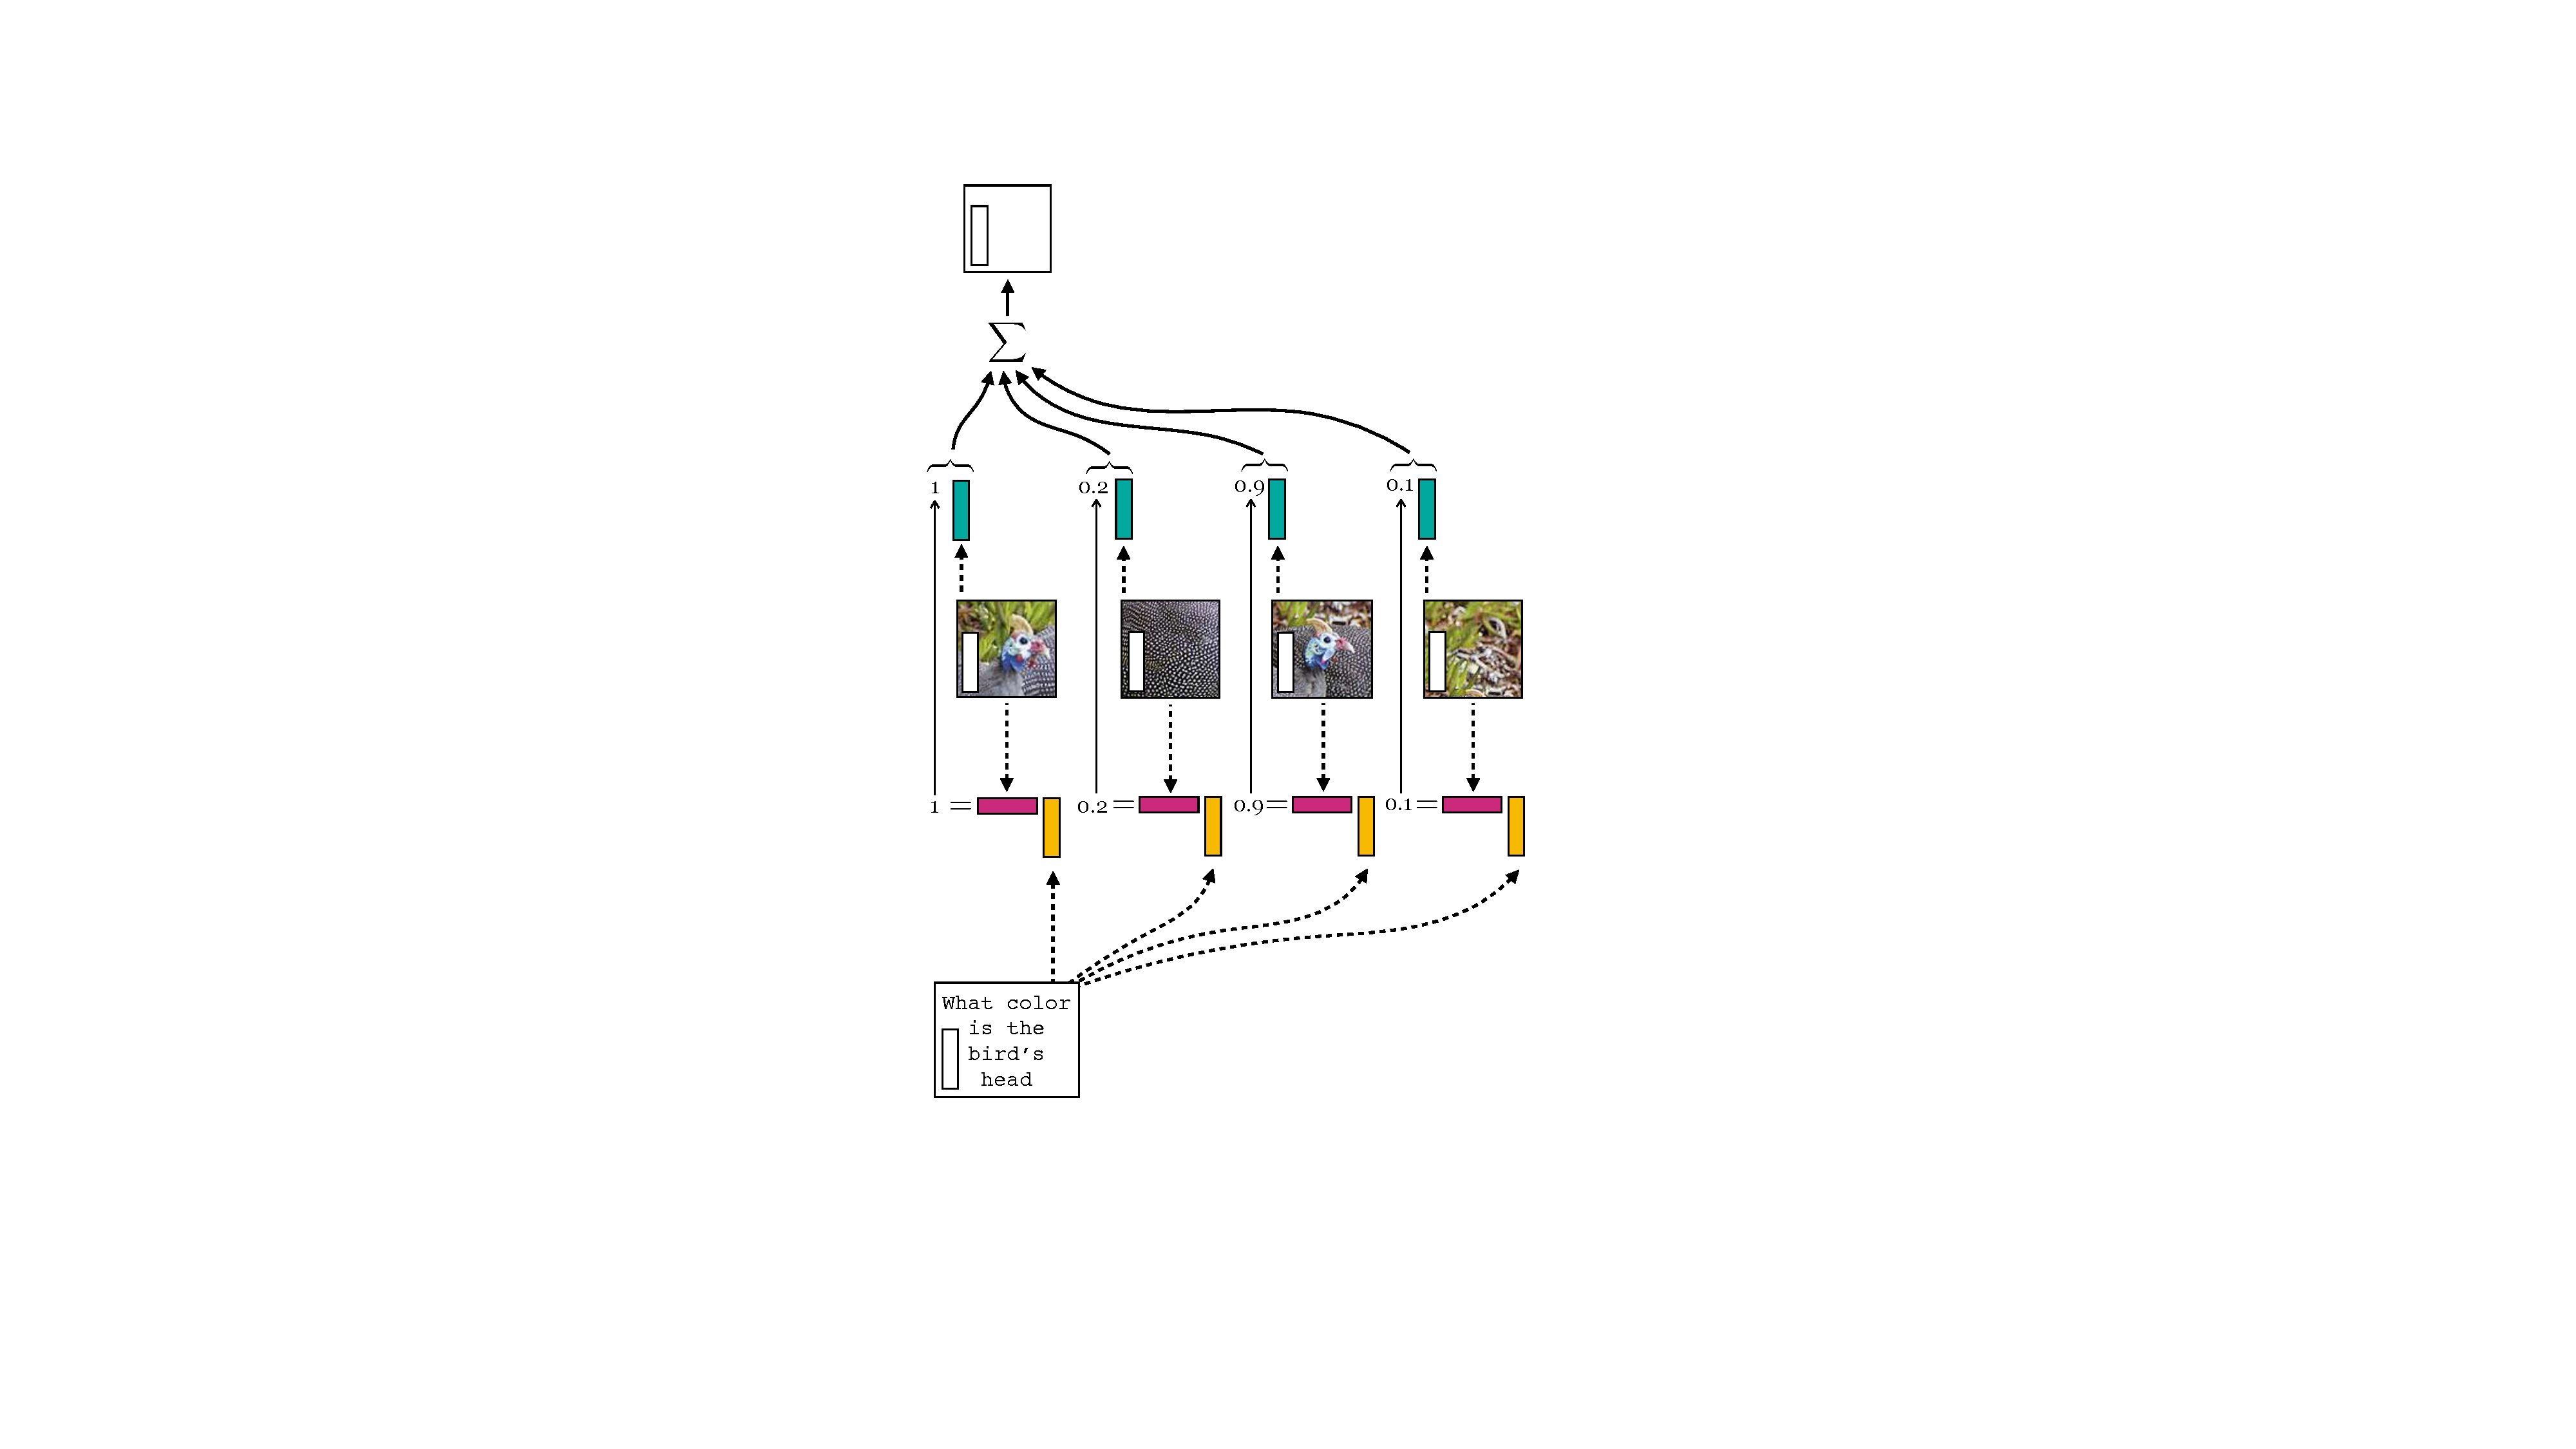
\includegraphics[width=0.4\linewidth]{./figures/transformers/attn_arch1.pdf}};
    \draw (-3.75, 0) node {$\tin$}; \draw (-3.25,-0.5) -- (-3.25,0.5);
    \draw (-3.75, 3.5) node {$t_\texttt{out}$}; \draw (-3.25,3.0) -- (-3.25,4.0);
    \draw (4, 0.75) node {$\} \quad \texttt{value()}$};
    \draw (4, -1) node {$\Big\} \quad \texttt{key()  }$};
    \draw (4, -2.5) node {$\Big\} \quad \texttt{query()}$};
\end{tikzpicture}
}
\caption{Mechanics of an attention layer. Queries from the question match keys from the tokens representing bird heads; value vectors of these two tokens then contribute the most to the sum that yields $t_{\texttt{out}}$'s code vector. (Softmax omitted in this example.)}
\label{fig:transformers:attn_arch1}
\end{figure}
\vspace{-0.2cm}

\subsection{Self-attention}
As we have now seen, attention is a general-purpose way of dynamically pooling information in one set of tokens based on queries from a different set of tokens. The next question we will consider is: ``which tokens should be doing the querying and which should we be matching against?" In the example from the last section, the answer was intuitive because we had a textual question that was asking about content in a visual image, so naturally the text gives the query and we match against tokens that represent the image. But can we come up with a more generic architecture where we don't have to hand design which tokens interact in which ways?

\marginnote{We use the following color scheme here and later in this chapter:
\medbreak
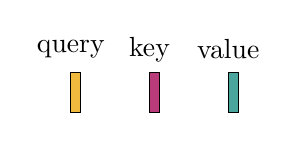
\begin{tikzpicture}
    \def\neuronrad{0.25}
    \draw [fill=query_color] (0,0) rectangle ++(\neuronrad/2,\neuronrad*2);
    \draw [fill=key_color] (1,0) rectangle ++(\neuronrad/2,\neuronrad*2);
    \draw [fill=value_color] (2,0) rectangle ++(\neuronrad/2,\neuronrad*2);
    %
    \draw (0,0.8) node {query};
    \draw (1,0.8) node {key};
    \draw (2,0.8) node {value};
\end{tikzpicture}
}[-4cm]

\textbf{Self-attention} is just such an architecture. The idea is that on a self-attention layer, \textit{all} tokens submit queries, and for each of these queries, we take a weighted sum over \textit{all} tokens in that layer. If $\tin$ is length $N$ then we have $N$ queries, $N$ weighted sums, and $N$ output tokens to form $\tout$:
\begin{figure}[h]
\centerline{
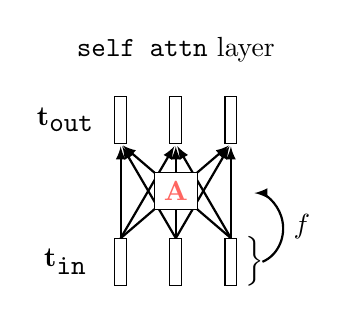
\begin{tikzpicture}
%
\def\Nnodes{3}
\def\Nlayers{2}
\def\layerheight{1.8}
\def\neuronrad{0.3}
\def\neuronstep{0.7}
\foreach \x in {1,...,\Nnodes} {
    \foreach \y in {1,...,\Nlayers} {
        \draw (\neuronstep*\x-\neuronrad/4,(\layerheight*\y-\layerheight-\neuronrad) rectangle ++(\neuronrad/2,\neuronrad*2);
    }
}
% mixing layer 1
\foreach \xi in {1,...,\Nnodes} {
    \foreach \xj in {1,...,\Nnodes} {
        \draw [thick] [nn_edge] (\neuronstep*\xi,\neuronrad) -- (\neuronstep*\xj,\layerheight-\neuronrad);
    }
}
%
\draw (1.4,0.5*\layerheight) node[draw,rectangle,fill=white] {$\color{data_color}\mathbf{A}$};
\draw (2.4, 0) node {$\Big\}$};
%\draw (2.4, 0.5*\layerheight) node {$\Bigg\}$};
%\draw [thick] [nn_edge] (2.5,0)  .. controls (2.7,0.25*\layerheight) .. (2.0,0.5*\layerheight);
\draw [thick] [nn_edge] (2.5,0) arc
    [
        start angle=-70,
        end angle=90,
        x radius=0.4cm,
        y radius =0.45cm
    ] ;
\draw (3.0,0.25*\layerheight) node {$f$};
\draw (1.4,1.5*\layerheight) node {\texttt{self attn} layer};
\draw (0,0) node {$\tin$};
\draw (0,1.8) node {$\tout$};
\end{tikzpicture}
}
\caption{A self-attention layer.}
\end{figure}
\vspace{-0.5cm}

%In the figure below we name the attention weight matrix as $\mathbf{A}$ (for ``affinity matrix", or, if you like ``attention matrix") and color it red since it is \textit{not} free learnable parameters but rather derived from \textit{activations} output by other parts of the network (which we will describe below):

The equations for self-attention can be written in an especially compact form:
\begin{align}
    \mathbf{Q}_{\texttt{in}} &= \Zin\mathbf{W}_q &\triangleleft \quad\quad \text{query matrix}\\
    \mathbf{K}_{\texttt{in}} &= \Zin\mathbf{W}_k &\triangleleft \quad\quad \text{key matrix}\\
    \mathbf{V}_{\texttt{in}} &= \Zin\mathbf{W}_v &\triangleleft \quad\quad \text{value matrix}\\
    \mathbf{A} &= f(\tin) = \texttt{softmax}(\frac{\mathbf{Q}_{\texttt{in}}\mathbf{K}_{\texttt{in}}^T}{\sqrt{d}}) &\triangleleft \quad\quad \text{attention matrix}\\
    \Zout &= \mathbf{A}\mathbf{V}_{\texttt{in}}
\end{align}
$d$ is dimensionality of the query/key vector (since we take a dot product between query and key their dimensionalities must match). In expanded detail, here are the full mechanics of an attention layer:
\begin{figure}[h]
\centerline{
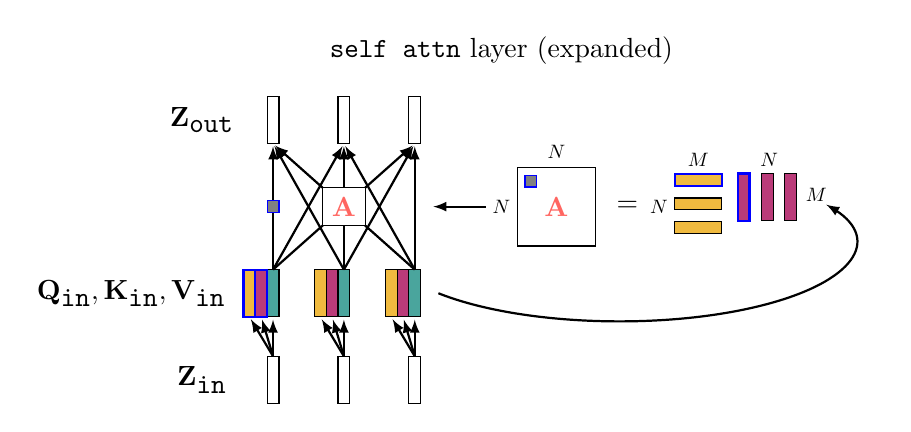
\begin{tikzpicture}
%
\def\Nnodes{3}
\def\Nlayers{2}
\def\layerheight{1.1}
\def\neuronrad{0.3}
\def\neuronstep{0.9}
% input layer
\foreach \x in {1,...,\Nnodes} {
    \def\y{1}
    \draw (\neuronstep*\x-\neuronrad/4,(\layerheight*\y-\layerheight-\neuronrad) rectangle ++(\neuronrad/2,\neuronrad*2);
}
% pointwise nonlinearity
\foreach \x in {1,...,\Nnodes} {
    \draw [thick] [nn_edge] (\neuronstep*\x,\neuronrad) -- (\neuronstep*\x,\layerheight-\neuronrad);
    \draw [thick] [nn_edge] (\neuronstep*\x,\neuronrad) -- (\neuronstep*\x-\neuronrad*0.5,\layerheight-\neuronrad);
    \draw [thick] [nn_edge] (\neuronstep*\x,\neuronrad) -- (\neuronstep*\x-\neuronrad,\layerheight-\neuronrad);
}
% query-key-value layer
\def\y{2}
\foreach \x in {1,...,\Nnodes} {
    \draw [fill=value_color] (\neuronstep*\x-\neuronrad/4,(\layerheight*\y-\layerheight-\neuronrad) rectangle ++(\neuronrad/2,\neuronrad*2);
    \draw [fill=key_color] (\neuronstep*\x-\neuronrad/4-\neuronrad*0.5,(\layerheight*\y-\layerheight-\neuronrad) rectangle ++(\neuronrad/2,\neuronrad*2);
    \draw [fill=query_color] (\neuronstep*\x-\neuronrad/4-\neuronrad,(\layerheight*\y-\layerheight-\neuronrad) rectangle ++(\neuronrad/2,\neuronrad*2);
}
\draw [fill=key_color, thick, draw=blue] (\neuronstep-\neuronrad/4-\neuronrad*0.5,(\layerheight*\y-\layerheight-\neuronrad) rectangle ++(\neuronrad/2,\neuronrad*2);
\draw [fill=query_color, thick, draw=blue] (\neuronstep-\neuronrad/4-\neuronrad,(\layerheight*\y-\layerheight-\neuronrad) rectangle ++(\neuronrad/2,\neuronrad*2);
    
\foreach \x in {1,...,\Nnodes} {
    \def\y{4}
    \draw (\neuronstep*\x-\neuronrad/4,(\layerheight*\y-\layerheight-\neuronrad) rectangle ++(\neuronrad/2,\neuronrad*2);
}
% attn
\def\y{1}
\foreach \xi in {1,...,\Nnodes} {
    \foreach \xj in {1,...,\Nnodes} {
        \draw [thick] [nn_edge] (\neuronstep*\xi,\layerheight*\y+\neuronrad) -- (\neuronstep*\xj,\layerheight*2+\layerheight*\y-\neuronrad);
    }
}
%
\draw (1.8,2*\layerheight) node[draw,rectangle,fill=white] {$\color{data_color}\mathbf{A}$};

\def\offset{0.6}
\draw (4, \offset+\layerheight) rectangle ++(1,1);
\draw (4+0.5, \offset+\layerheight+0.5) node {$\color{data_color}\mathbf{A}$};
\draw [fill=gray, draw=blue] (4+0.1, \offset+\layerheight+1-0.25) rectangle ++(\neuronrad/2,\neuronrad/2);
\draw [fill=gray, draw=blue] (\neuronstep-\neuronrad/4, 2*\layerheight-\neuronrad/4) rectangle ++(\neuronrad/2,\neuronrad/2);
\draw (4+0.5, \offset+\layerheight+1+0.2) node[scale=0.7] {$N$};
\draw (4-0.2, \offset+\layerheight+0.5) node[scale=0.7] {$N$};
\draw (4+1+0.4, \offset+\layerheight+0.5) node {$=$};
\foreach \x in {1,...,\Nnodes} {
    \draw [fill=query_color] (6,\offset+\layerheight+\x*0.3+0.06-0.2) rectangle ++(\neuronrad*2,\neuronrad/2);
    
    \draw [fill=key_color] (6.7+\x*0.3-0.2,\offset+\layerheight+0.32) rectangle ++(\neuronrad/2,\neuronrad*2);
}

\draw [fill=query_color, draw=blue, thick] (6,\offset+\layerheight+0.3*3+0.06-0.2) rectangle ++(\neuronrad*2,\neuronrad/2);
\draw [fill=key_color, draw=blue, thick] (6.7+0.3-0.2,\offset+\layerheight+0.32) rectangle ++(\neuronrad/2,\neuronrad*2);

\draw (5.8, \offset+\layerheight+2*0.2+0.1) node[scale=0.7] {$N$};
\draw (6.3, \offset+\layerheight+4*0.2+0.3) node[scale=0.7] {$M$};
\draw (7.2, \offset+\layerheight+4*0.2+0.3) node[scale=0.7] {$N$};
\draw (7.8, \offset+\layerheight+2*0.2+0.25) node[scale=0.7] {$M$};
\draw [thick] [nn_edge] (3,\layerheight) arc
    [
        start angle=-140,
        end angle=30,
        x radius=3.0cm,
        y radius =1.0cm
    ] ;
\draw [thick] [nn_edge] (3.6,\layerheight+\offset+0.5) -- (2.9,\layerheight+\offset+0.5);

\draw (3.8,3.8*\layerheight) node {\texttt{self attn} layer (expanded)};
\draw (0,0) node {$\Zin$};
\draw (0,\layerheight*3) node {$\Zout$};
\draw (-0.9,\layerheight) node {$\Qin, \Kin, \Vin$};
\end{tikzpicture}
}
\caption{Self-attention layer expanded. The nodes outlined in blue correspond to each other; they represent one query being matched against one key to result in a scalar similarity value, in the gray box, which acts as a weight in the weighted sum computed by $\mathbf{A}$.}
\label{fig:transformers:attn_arch}
\end{figure}
% \begin{figure}[h]
%     \centering
%     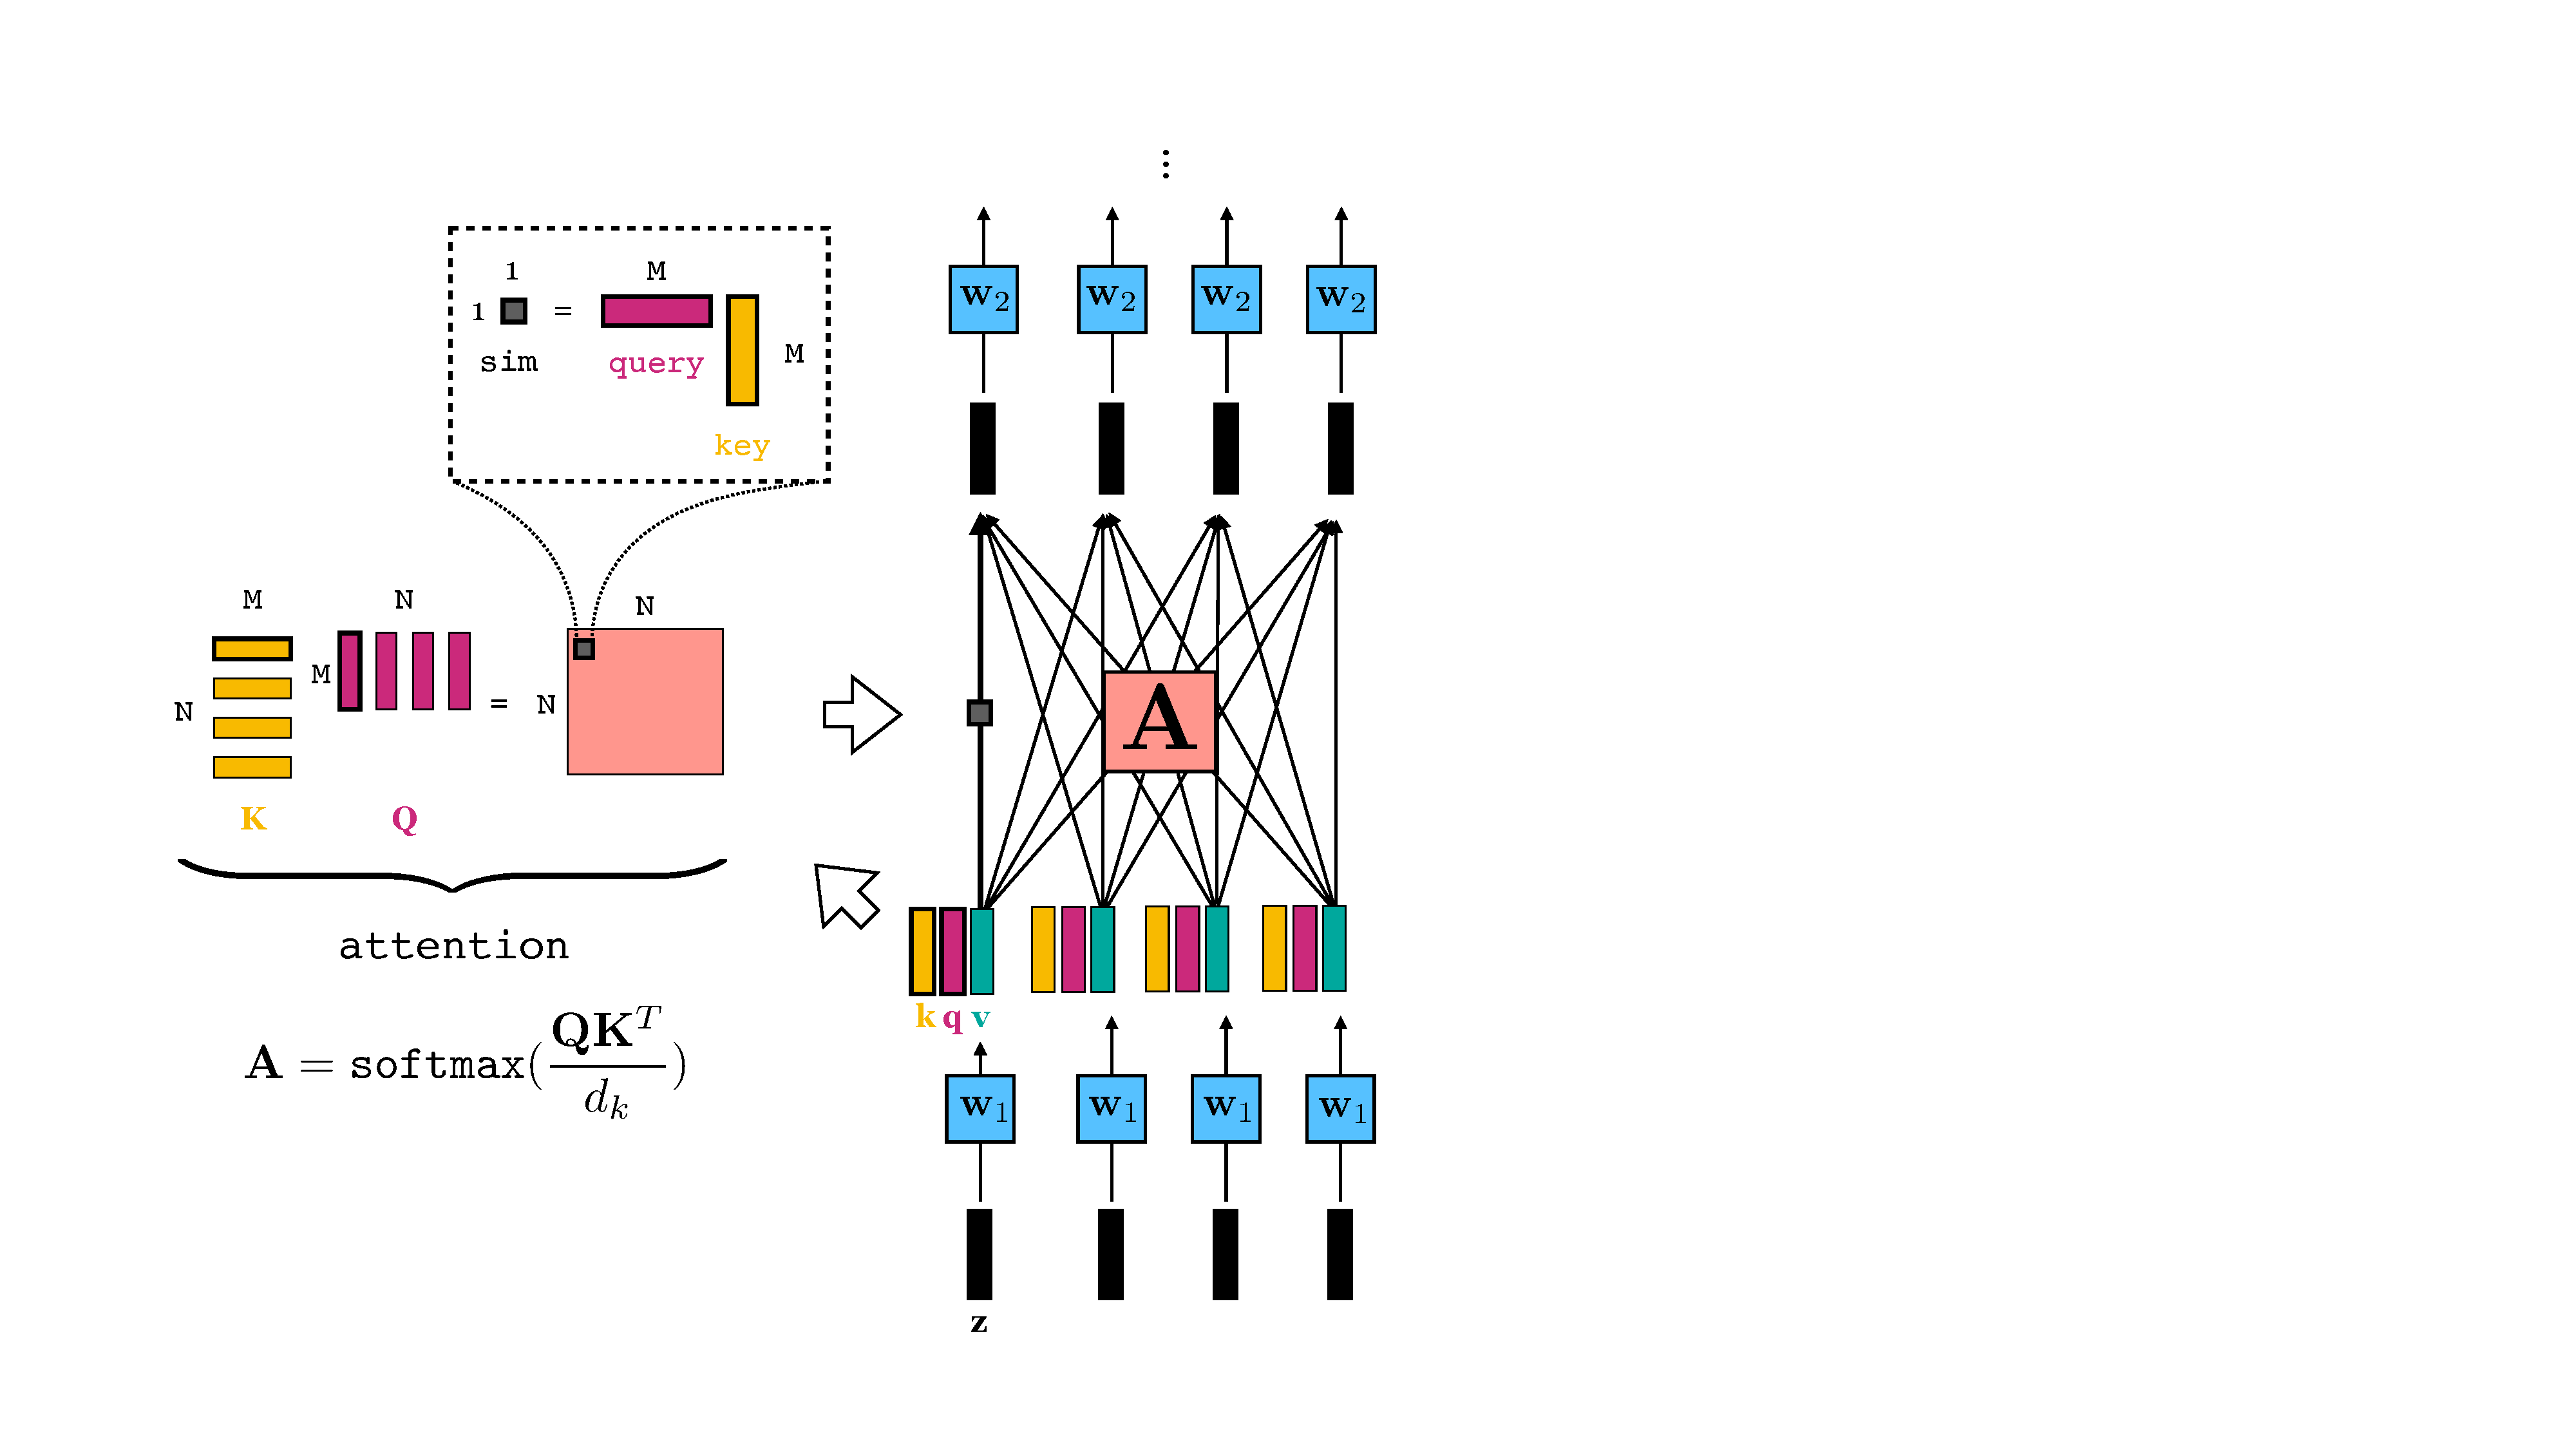
\includegraphics[width=0.6\linewidth]{./figures/transformers/attn_arch.pdf}
%     \label{fig:transformers:attn_arch}
% \end{figure}

This fully defines a self-attention layer, which is the kind of attention layer used in transformers. Before we move on though, let's think through the intuition of what self-attention might be doing.

Consider that we are processing the Guineafowl image and our task is semantic segmentation (label each patch with an object class). First, we tokenize the image so that each patch is represented by a token. Now we have a token, $t_1$, that represents the patch of pixels around of the birds' heads. We wish to update this token via one layer of self-attention. Since the goal of the network is to classify patches, it would make sense to update $t_1$ to get a better semantic representation of what's going on in that patch. One way to do this would be to attend to the tokens representing the other bird heads, and use them to refine $t_1$. The intuition is that it's easier to recognize an object given three views of it (the three tokens representing bird heads). The refinement operation is just to sum over the token code vectors, which has the effect of reducing ``noise" that is not shared between the three tokens and amplifying the commonalities between them. Figure \ref{fig:attention_layer_cartoon} illustrates this scenario.

\begin{figure}[h!]
\centerline{
\begin{tikzpicture}
    \draw (0, 0) node[inner sep=0] {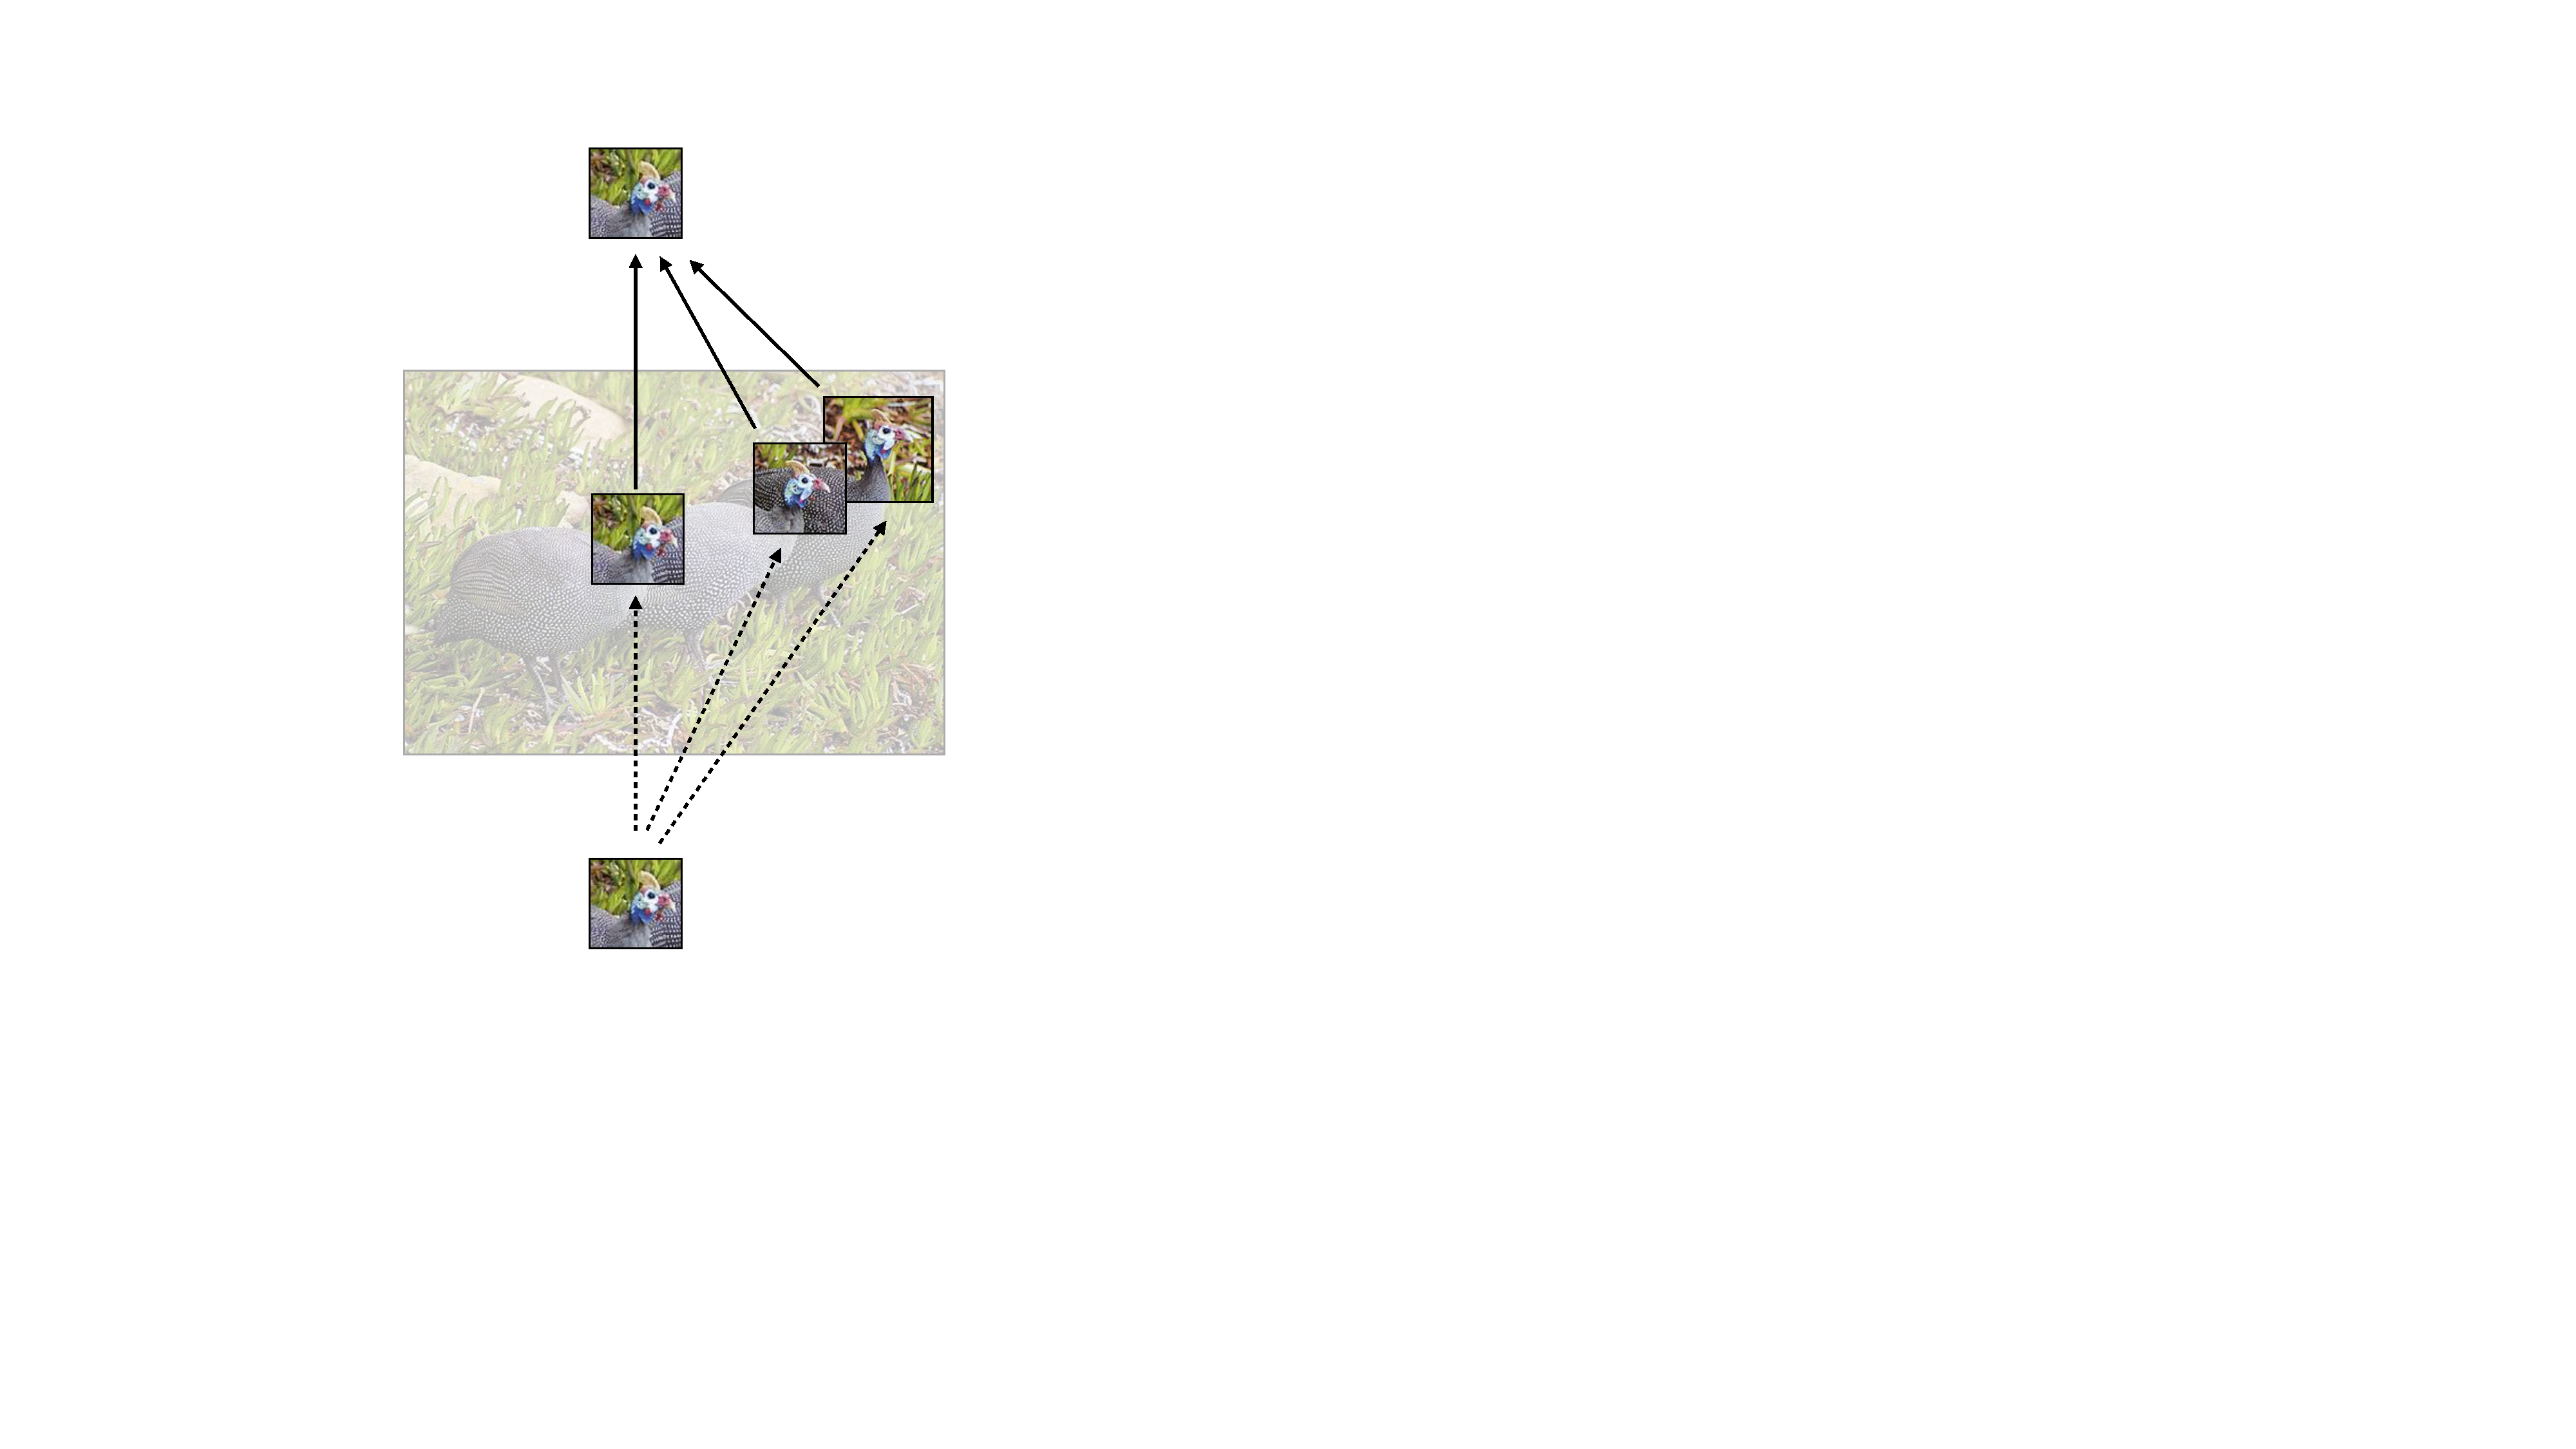
\includegraphics[width=0.45\linewidth]{./figures/transformers/attention_layer_cartoon.pdf}};
    \draw (-0.8, -3.1) node [draw,rectangle,fill=white] {$t_1$};
    \draw (-0.8, 0.6) node [draw,rectangle,fill=white] {$t_1$};
    \draw (-0.8, 4) node [draw,rectangle,fill=white] {$t_1$};
    \draw (0.8, 1) node [draw,rectangle,fill=white] {$t_2$};
    \draw (1.5, 1.5) node [draw,rectangle,fill=white] {$t_3$};
    \draw (2.25,-1.5) node {\texttt{attention}};
     \draw (1.25,2.5) node {\texttt{sum}};
\end{tikzpicture}
}
\caption{One way self-attention could be used to aggregate information across all patches containing the same object, and thereby arrive at a better representation of this object.}
\label{fig:attention_layer_cartoon}
\end{figure}

This is just one way self-attention could be used by the network. How it is actually used will be determined by the training data and task. What really happens might deviate from our intuitive story: tokens on hidden layers do not necessarily represent spatially localized patches of pixel. While the initial tokenization converts patches to pixels, after this point attention layers can mix information across spatially distant tokens -- $t_{\texttt{out}}_1$ does not necessarily represent the same spatial region in the image as $t_{\texttt{in}}_1$.

In fact, attention layers are \textbf{permutation equivariant}:
\begin{align}
    \texttt{attn}(\texttt{permute}(\tin)) = \texttt{permute}(\texttt{attn}(\tin))
\end{align}
where $\texttt{permute}$ is a permutation of the indices of the vector $\tin$. This means that if you scramble (i.e. permute) the patches in the input image then apply attention, the output will be unchanged up to a permutation of the original output. It is often useful to understand layers in terms of their invariances and equivariances. Convolutational layers are translation equivariant but not necessarily permutation equivariant whereas attention layers are both translation equivariant \textit{and} permutation equivariant (since translation is a special kind of permutation, any permutation equivariant layer is also translation equivariant). Note, however, that 1x1 convolutions are a special case of convolution that is in fact permutation equivariant, because they are operate pointwise. Other layers can be catalogued similarly: global average pooling layers are permutation \textit{invariant}, relu layers are permutation equivariant, per-token MLP layers are also permutation equivariant (but w.r.t. vectors of tokens rather than vectors of neurons), and so on. As we will see below, all layers in standard transformers are permutation equivariant, so the entire transformer is permutation equivariant over its input tokens.

A generally good strategy is to select layers that reflect the symmetries in your data domain or task: in object detection, translation equivariance makes sense because, roughly, a bird is a bird no matter where it appears in an image. Permutation equivariance might also make sense, for that same reason, but only to an extent: if you break up an image into small patches and scramble them then this could disrupt spatial layout that is important for recognition. We will see in Section \ref{sec:transformers:positional_encodings} how transformers use something called positional codes to re-insert useful information about spatial layout.

%To do so, $t_1$ may allocate attention over other regions of the image that it deems are relevant to understanding the bird's head. Since there are three birds, it would make sense for the $t_1$ to attend to the tokens that represent the other heads. This way it could aggregate the information 

%The way $t_1$ uses its attention is simply to take a weighted sum over the tokens it is attending to. This sum is a summary of all the information being attended to. $t_1$ will then update its code by adding in this weighted sum over the codes of all the tokens it is attending to.


% Let's consider just one token in the input; the steps we describe next will be applied to each token in the same way. To anthropomorphize for a minute, the token's goal is to improve it's representation by mixing in information from the other tokens in the input. The token first \textbf{queries} the other tokens, asking ``which of you match my query". The query is vector output as a function of the token's internal vector. The query vector is matched against the \textbf{key} vector of each token in the input vector of tokens. The best matching tokens submit a response as a \textbf{value} vector to be averaged into the querier's internal vector.

% We will create a matrix $\mathbf{S}$ of the similarity between $\mathbf{q}_{t}$ and $\mathbf{k}_{t_{\texttt{in}_i}}$ for all tokens $t_{\texttt{in}_i}$:
% \begin{align}
%     \mathbf{S}_i = \texttt{sim}(\mathbf{q}_{t}, \mathbf{k}_{t_{\texttt{in}_i}})
% \end{align}




% \begin{align}
%     t_1 \leftarrow w_1 t_1 + w_2 t_2 + w_3 t_3
% \end{align}

%\textbf{Attention layers} can be easily understood by starting with the linear combination of tokens defined above. An attention layer is simply an linear layer whose weights are determined as \textit{functions of the data}. The intuition is that this function decides what parts of the input to ``attend" to in producing the output representation. 

%If a weight between an input and output token is near-zero, then that input is ignored; if the weight is high then that input is attended to.



% \begin{figure}[h]
%     \centering
%     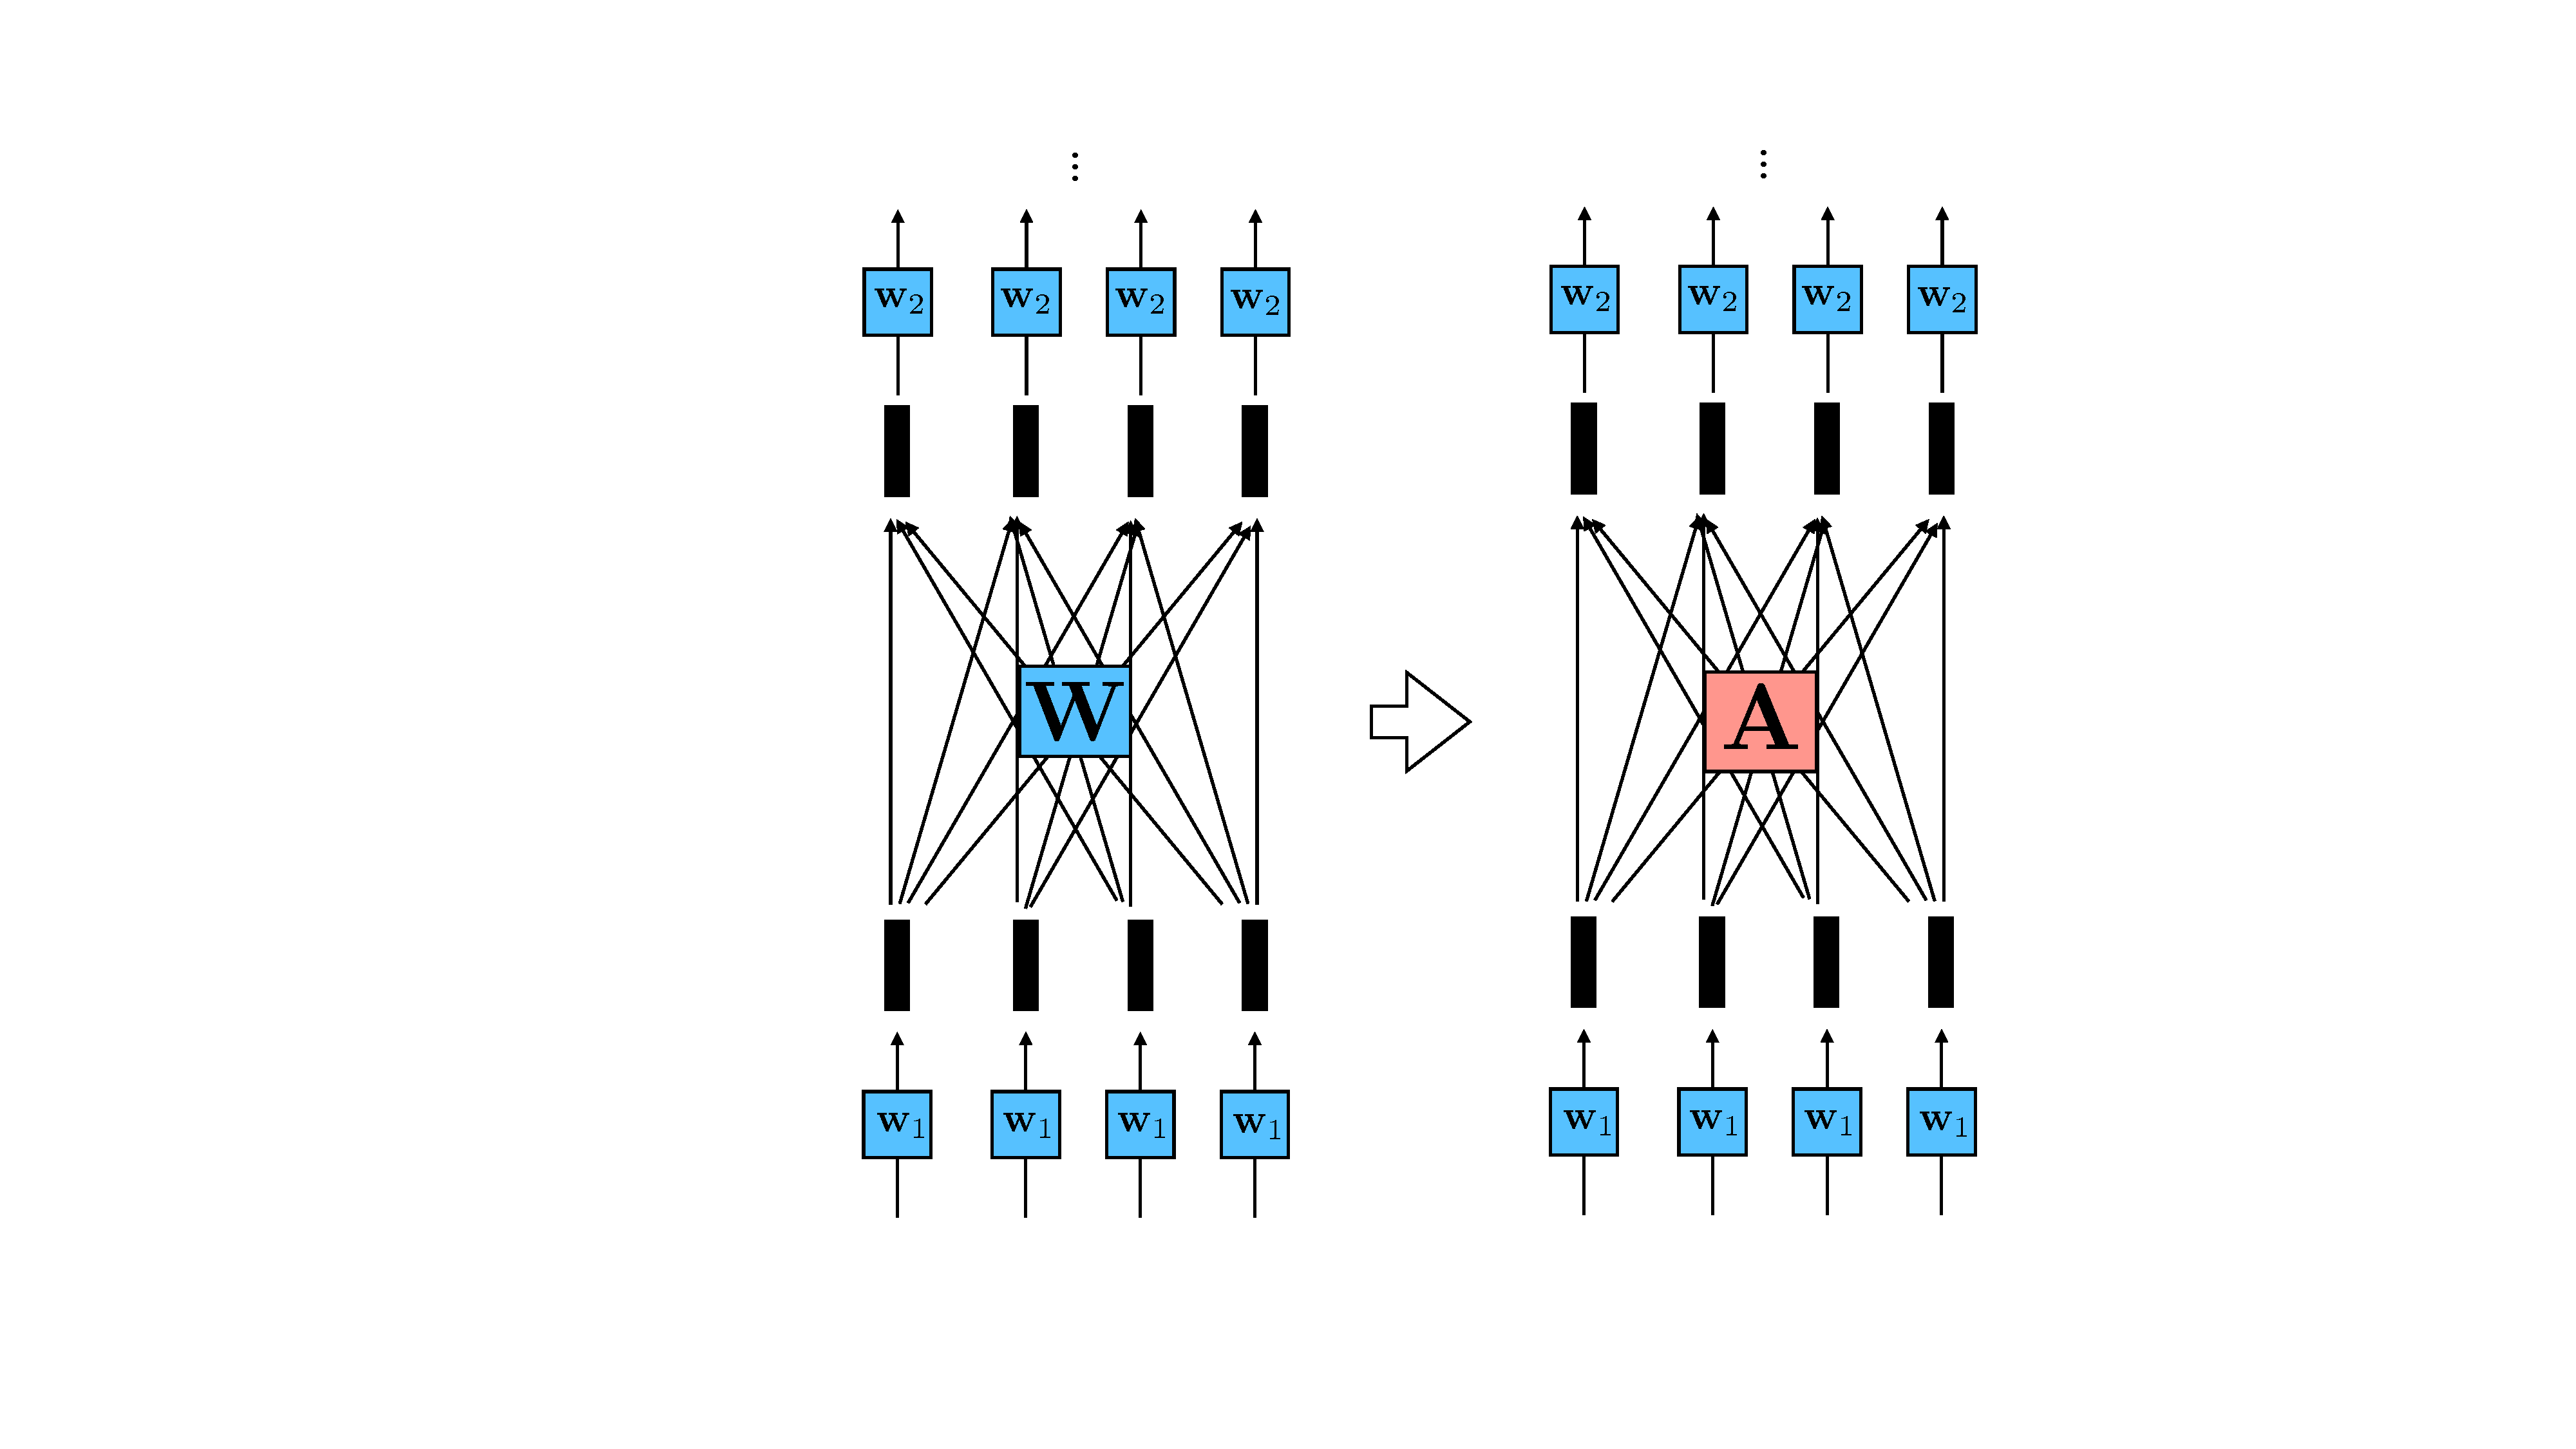
\includegraphics[width=0.6\linewidth]{./figures/transformers/fc_to_attn.pdf}
%     \label{fig:transformers:fc_to_attn}
% \end{figure}

%Rather than applying \textit{the same} filter to different locations in a signal, transformers apply a \textit{dynamic filter} that is different at each different location. However, the dynamics that determine the filter weights \textit{are the same} across locations! So we have something like Property \#2 of CNNs (see Chapter XX), except at an abstracted level: the weights are not shared but how the weights are determined is shared.

%The workhorse of transformers is {\bf self-attention layers}. These layers take a set of {\bf tokens} as input and produce a transformed set of tokens as output. A ``token" is simply transformer lingo for a vector. The set of tokens need not have any ordering -- all the computations over tokens can occur in parallel. Just like with ``patches" in a CNN, each token is processed in a manner that is independent and identical to how all the other tokens are processed.

% You are probably wondering: what is $f$ in the figure above? Well, since $\mathbf{A}$ is not free parameters, its value has to be some other way. What we have depicted above is \textbf{self-attention} where $\mathbf{A}$ is determined by a function $f$ of the \textit{inputs to the attention layer themselves}:
% \begin{align}
%     \mathbf{A} &= f(\tin, \ldots)  \quad\quad \triangleleft \text{ self-attention}\\
%     \Xout &= \mathbf{A}\tin
% \end{align}

% Transformers use self-attention layers like this. In general, however, the attention weights $\mathbf{A}$ could be determined in other ways, for example, an external signal or a separate branch of the computation graph could be the inputs to $f$ that determines $\mathbf{A}$. In general, an attention layer can be any linear layer where the \textit{weights} are \textit{data-dependent}, that is, they are determined as the \textit{output activations} of data processing by some other module of the computation graph\marginnote{In this way, the parameters of the net $\mathbf{A}$ are the outputs of another net $f$. A net that parameterizes another net is sometimes called a hypernet~\cite{XX}, so attention is a hypernet~\cite{XX}.}[-0.4cm]:
% \begin{align}
%     \mathbf{A} &= f(\ldots) \quad\quad \triangleleft \text{ attention}\\
%     \Xout &= \mathbf{A}\tin
% \end{align}
% The interesting thing about attention is that it mixes the concepts of weights and activations, which previously we had kept separate.

% \subsection{Query-Key-Value attention}
% Transformers use a particular kind of self-attention based on the idea of keys, queries, and values from the information retrieval literature.

% Let's consider just one token in the input; the steps we describe next will be applied to each token in the same way. To anthropomorphize for a minute, the token's goal is to improve it's representation by mixing in information from the other tokens in the input. The token first \textbf{queries} the other tokens, asking ``which of you match my query". The query is vector output as a function of the token's internal vector. The query vector is matched against the \textbf{key} vector of each token in the input vector of tokens. The best matchig tokens submit a respose as a \textbf{value} vector to be averaged into the querier's internal vector.
% \begin{figure}
%     \centering
%     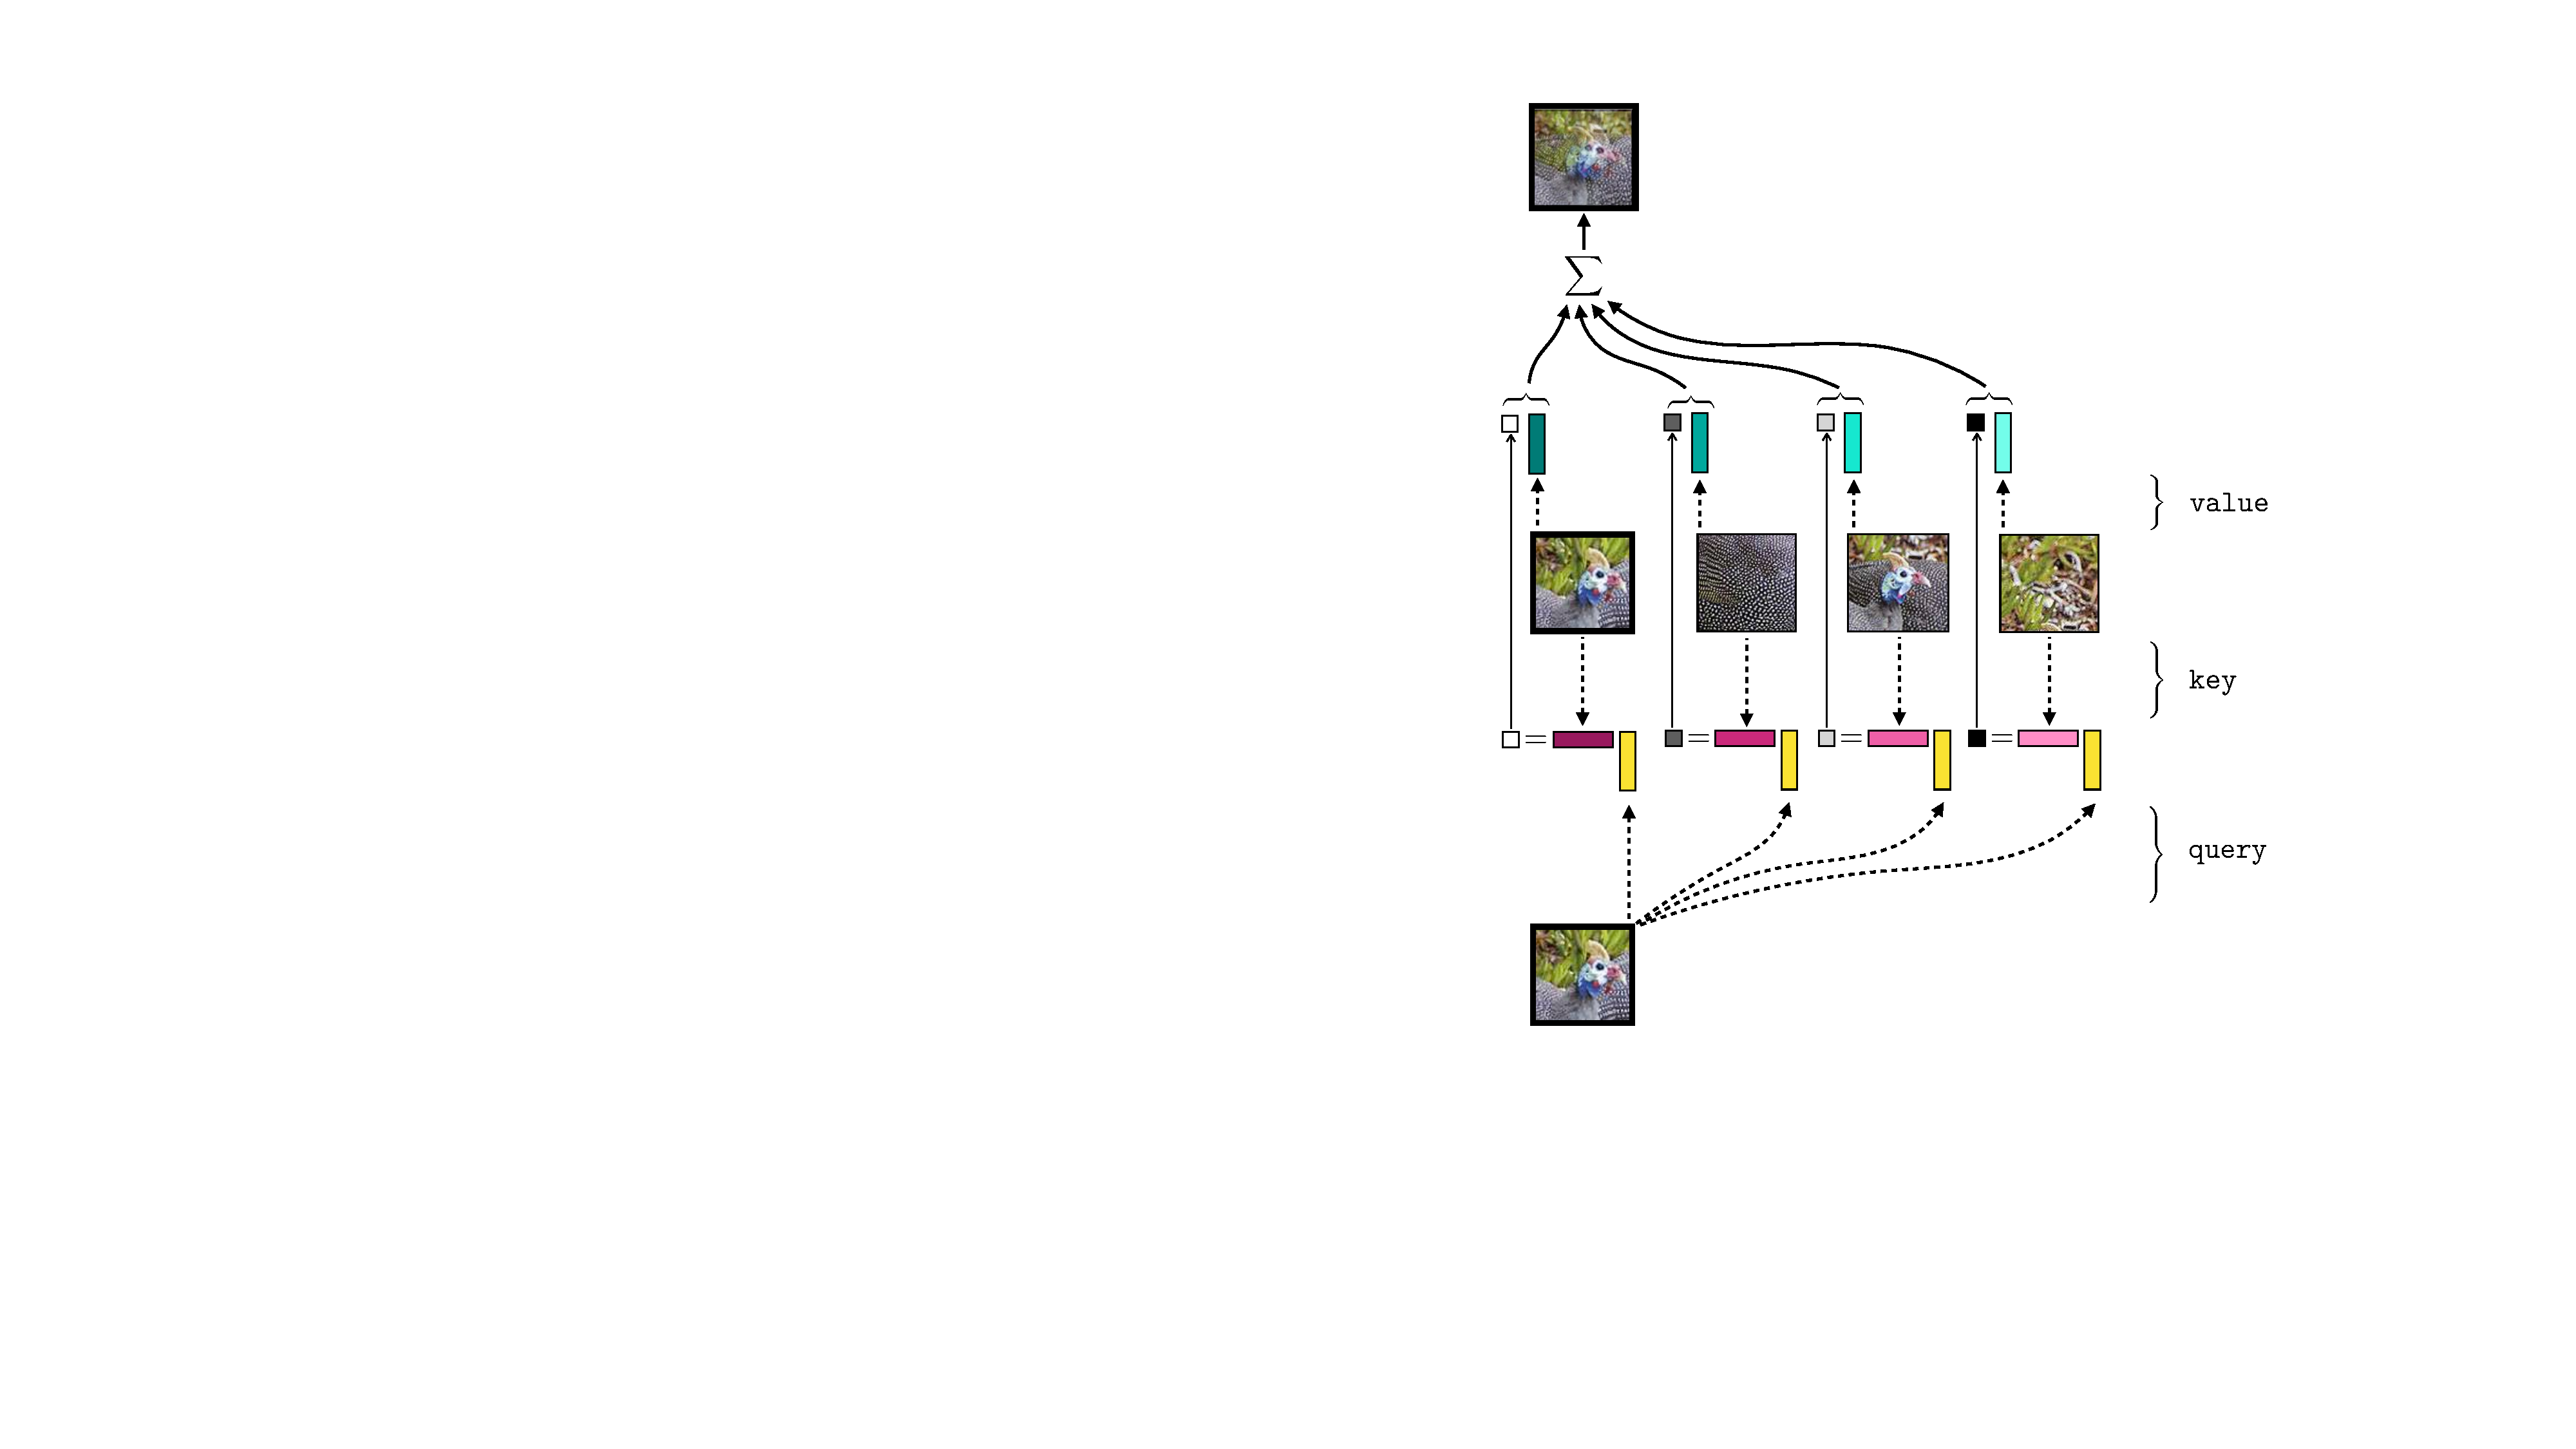
\includegraphics[width=0.5\linewidth]{./figures/transformers/attention_layer_1_token.pdf}
%     \label{fig:attention_layer_1_token}
% \end{figure}


% To motivate self-attention, we will start with a stripped down version. 
% %Let $\Xin \in \mathbb{R}^{N \times M}$ denote $N$ input tokens each of which is a $1 \times M$ dimensional vector. $\Xout$ is the corresponding array of transformed output tokens. Then a simple kind of self-attention layer can be defined by the following operations:
% Suppose we have a vector of tokens, $\tin$ as input to our self-attention layer. First, we measure the similarity between each token in the vector and every other token in the vector. Our notion of similarity between two tokens will be their inner product. Using our notation for tokens, the matrix of all the inner products between the input tokens can be compactly written as an outer-product:
% \begin{align}
%     %\mathbf{G} &= \Xin\Xin^T\\
%     \mathbf{G} &= \tin\tin^T
% \end{align}
% %$\mathbf{G}$$ is a \textbf{Gram matrix} -- a matrix of inner products between all elements in a vector.
% $\mathbf{G}$ is the Gram matrix over tokens; it measures the similarity (dot product) between all pairs of tokens. We will use this similarity matrix to determine the amount of ``attention" each token pays to each other token. 

% We want to use these values to decide how much attention each token should pay to each other token. Intuitively, we want the amount of total attention to be a constant value and the weights to be nonnegative, so we will pass $\mathbf{G}$ through a softmax to obtain our affinity matrix $\mathbf{A}$:
% \begin{align}
%     \mathbf{A} &= \texttt{softmax}(\mathbf{G})\Y \quad\quad \triangleleft \text{ softmax over rows}\\
%     \tout &= \mathbf{A}\tin
% \end{align}



% If we then pass each row of $\mathbf{G}$ through a $\texttt{softmax}$ function then we can interpret each softmaxed row as a normalized set of non-negative weights that we will use in a weighted sum over tokens, i.e. our affinity matrix $\mathbf{A}$. Finally we compute this weighted sum as $\tout = \mathbf{A}\tin$. The output tokens are weighted sums of the input tokens, weighted by the similarity of each input token with each other input token. This layer will act to cluster the tokens since similar tokens end up being averaged together and that results in them becoming more similar to each other.

% We will make this clearer graphically. We will focus on how the self-attention layer updates just one token, $\xin \rightarrow \xout$:


% \begin{figure}[h]
% \centering
% \begin{tikzpicture}
%     \def\neuronrad{0.35}
%     \draw [fill=blue] (0,0) rectangle ++(\neuronrad/2,\neuronrad*2);
%     %
%     \draw (0,1) node {$\xout = \sum_{i=1}^N a_i \Xin[i,:]$}
% \end{tikzpicture}
% \end{figure}

% If we want to do more than just clustering, we can introduce additional transformations, which will yield the canonical self-attention layers used in transformers.
% \begin{align}
%     \mathbf{Q} &= \Xin\mathbf{W}^q &\triangleleft \quad\quad \texttt{query}\\
%     \mathbf{K} &= \Xin\mathbf{W}^k &\triangleleft \quad\quad \texttt{key}\\
%     \mathbf{V} &= \Xin\mathbf{W}^v &\triangleleft \quad\quad \texttt{value}\\
%     \Xout &= \texttt{softmax}(\frac{\mathbf{Q}\mathbf{K}^T}{d_k})\mathbf{V}
% \end{align}
% Notice that $\Xin\mathbf{W}^q = \sum_{c=1}^C \mathbf{W}^q_{k,c} \star \mathbf{X}_{\texttt{in}_c}$, which, referring back to Chapter \ref{chapter:convolutional_neural_nets} can be identified as a multi-channel convolution layer (without a bias). This reveals a connection between transformers and CNNs: the query, key, and value in transformers is arrived at by convolving the input set of tokens with a learned set of filters (the convolution kernels in this case are $1 \times 1$ in the ``spatial", cross-token, domain). All these operations happen independently and identically at the token level. Then the attention matrix is just a linear layer on top. This linear layer is data dependent because its weights are constructed from the tokens. %That data-dependency shares a property with an RNN: it can model bilinear dependencies over signals of unbounded length, whereas CNNs can only model local dependencies.

%\subsection{Multi-headed attention}

%The transformer encoder blocks defined in \cite{vaswani2017attention} operate as follows:
%\begin{align}
%    \texttt{MSH}(\Xin)
%\end{align}

\section{The full transformer architecture}

%The transformer architecture consists of a sequence of {\bf transformer encoder} blocks, each of which relies on self-attention layers. Just like a self-attention layer, each transformer encoder takes a set of $N$ tokens as input and produces a set of $N$ tokens as output.

A full transformer architecture is a stack of self-attention layers interleaved with token-wise nonlinearities. These two steps are analogous to linear layers interleaved with neuron-wise nonlinearities in an MLP:
\begin{figure}[h]
\centerline{
\begin{minipage}{.49\linewidth}
\centering
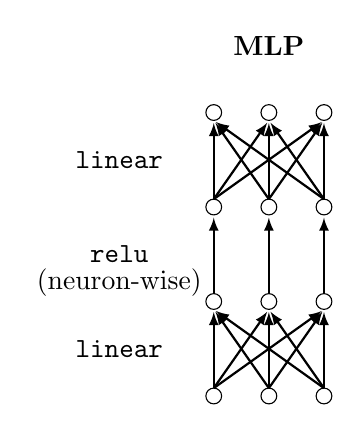
\begin{tikzpicture}
%
\def\Nnodes{3}
\def\Nlayers{4}
\def\layerheight{1.2}
\def\neuronrad{0.1}
\def\neuronstep{0.7}
\foreach \x in {1,...,\Nnodes} {
    \foreach \y in {1,...,\Nlayers} {
        \draw (\neuronstep*\x,(\layerheight*\y-\layerheight) circle (\neuronrad);
    }
}
% mixing layer 1
\foreach \xi in {1,...,\Nnodes} {
    \foreach \xj in {1,...,\Nnodes} {
        \draw [thick] [nn_edge] (\neuronstep*\xi,\neuronrad) -- (\neuronstep*\xj,\layerheight-\neuronrad);
    }
}
% pointwise nonlinearity
\foreach \x in {1,...,\Nnodes} {
    \draw [thick] [nn_edge] (\neuronstep*\x,\layerheight+\neuronrad) -- (\neuronstep*\x,\layerheight*2-\neuronrad);
}
% mixing layer 2
\foreach \xi in {1,...,\Nnodes} {
    \foreach \xj in {1,...,\Nnodes} {
        \draw [thick] [nn_edge] (\neuronstep*\xi,\layerheight*2+\neuronrad) -- (\neuronstep*\xj,\layerheight*3-\neuronrad);
    }
}
%
\draw (\neuronstep*2,3.7*\layerheight) node {\textbf{MLP}};
\draw (-0.5,0.5*\layerheight) node {\texttt{linear}};
\draw (-0.5,1.5*\layerheight) node {\texttt{relu}};
\draw (-0.5,1.2*\layerheight) node {(neuron-wise)};
\draw (-0.5,2.5*\layerheight) node {\texttt{linear}};
\end{tikzpicture}
\end{minipage}
\begin{minipage}{.49\linewidth}
\centering
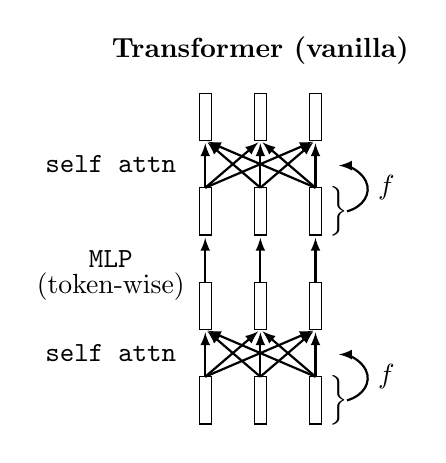
\begin{tikzpicture}
%
\def\Nnodes{3}
\def\Nlayers{4}
\def\layerheight{1.2}
\def\neuronrad{0.3}
\def\neuronstep{0.7}
\foreach \x in {1,...,\Nnodes} {
    \foreach \y in {1,...,\Nlayers} {
        \draw (\neuronstep*\x-\neuronrad/4,(\layerheight*\y-\layerheight-\neuronrad) rectangle ++(\neuronrad/2,\neuronrad*2);
    }
}
% mixing layer 1
\foreach \xi in {1,...,\Nnodes} {
    \foreach \xj in {1,...,\Nnodes} {
        \draw [thick] [nn_edge] (\neuronstep*\xi,\neuronrad) -- (\neuronstep*\xj,\layerheight-\neuronrad);
    }
}
% pointwise nonlinearity
\foreach \x in {1,...,\Nnodes} {
    \draw [thick] [nn_edge] (\neuronstep*\x,\layerheight+\neuronrad) -- (\neuronstep*\x,\layerheight*2-\neuronrad);
}
% mixing layer 2
\foreach \xi in {1,...,\Nnodes} {
    \foreach \xj in {1,...,\Nnodes} {
        \draw [thick] [nn_edge] (\neuronstep*\xi,\layerheight*2+\neuronrad) -- (\neuronstep*\xj,\layerheight*3-\neuronrad);
    }
}
\draw [thick] [nn_edge] (2.5,0) arc
    [
        start angle=-70,
        end angle=90,
        x radius=0.4cm,
        y radius =0.3cm
    ] ;
\draw [thick] [nn_edge] (2.5,\layerheight*2) arc
    [
        start angle=-70,
        end angle=90,
        x radius=0.4cm,
        y radius =0.3cm
    ] ;
\draw (2.4, 0) node {$\Big\}$};
\draw (2.4, \layerheight*2) node {$\Big\}$};
\draw (3.0,0.25*\layerheight) node {$f$};
\draw (3.0,0.25*\layerheight+\layerheight*2) node {$f$};
%
\draw (\neuronstep*2,3.7*\layerheight) node {\textbf{Transformer (vanilla)}};
\draw (-0.5,0.5*\layerheight) node {\texttt{self attn}};
\draw (-0.5,1.5*\layerheight) node {\texttt{MLP}};
\draw (-0.5,1.2*\layerheight) node {(token-wise)};
\draw (-0.5,2.5*\layerheight) node {\texttt{self attn}};
\end{tikzpicture}
\end{minipage}
}
\caption{The transformer architecture vs an MLP.}
\end{figure}

Beyond this basic template, there are many variations that can be added, resulting in different particular architectures within the transformer family. Some common additions are normalization layers and residual connections. 

\subsection{Multihead self-attention}
Additionally, it is common to use \textbf{multihead self-attention}, or \textbf{MSA}, which simply consists of running $k$ attention layers in parallel, applied to the same input $\tin$, then concatenating all the outputs, and finally projecting back to the original dimensionality of $\tin$:
\begin{align}
    \tout^i &= \texttt{attn}_i(\tin) \quad \forall i\\
    \mathbf{Z} &= \begin{pmatrix}
        \tout^1[1].\mathbf{z} & \ldots & \tout^k[1].\mathbf{z}\\
        \vdots & \vdots & \vdots \\
        \tout^1[N].\mathbf{z} & \ldots & \tout^k[N].\mathbf{z}\\
    \end{pmatrix} &\quad\quad \triangleleft \quad \mathbf{Z} \in \mathbb{R}^{N \times kM_1}\\
    \bar{\mathbf{Z}} &= \mathbf{Z}\mathbf{W} &\quad\quad \triangleleft \quad \mathbf{W} \in \mathbb{R}^{kM_1 \times M_2} \label{eqn:transformers:MSH}\\
    \tout[i].\mathbf{z} &= \bar{\mathbf{Z}}[i,:]
\end{align}
$\mathbf{W}$ are learnable parameters of this layer (in addition to the query, key, and value projections parameters for each of the $k$ attention heads), $M_1$ is the dimensionality of the value vectors and $M_2$ is the dimensionality of the code vectors of the output (\cite{dosovitskiy2020vit} recommends setting $kM_1 = M_2$).

\subsection{Masked attention}
Sometimes we want to restrict which tokens can attend to which. This can be done by \textit{masking} the attention matrix, which just means fixing some of the weights to be zero. This can be useful for many settings, including learning features via masked autoencoding~\cite{he2022masked}, cross-attention between different data modalities~\cite{wei2020multi}, and for sequential prediction~\cite{chen2020generative}. To illustrate, we will describe the sequential prediction use case.

A common problem is to predict the $(n+1)^{\text{th}}$ token in a sequence given the previous $n$ tokens. For example, we may be trying to predict tokens that represent the next frame in a video, the next word in a sentence, or the weather on the next day.

A simple way to model this prediction problem is with a linear layer: $t_{n+1} = \mathbf{W}\mathbf{t}_{-n}$.\marginnote{$\mathbf{t}_{-n}$ is shorthand for the vector of tokens $[t_1, \ldots, t_{n}]$}. Here is what this looks like diagrammatically, and on the right is the layer shown as matrix multiplication:
\begin{figure}[h]
\centerline{
\begin{minipage}{.49\linewidth}
\centering
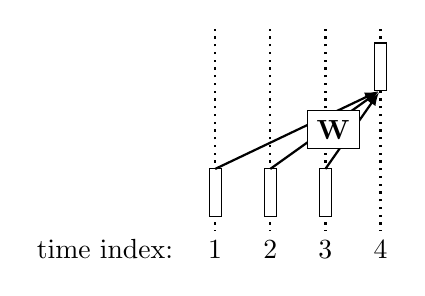
\begin{tikzpicture}
%
\def\Nnodes{3}
\def\Nnodesplusone{4}
\def\layerheight{1.6}
\def\neuronrad{0.3}
\def\neuronstep{0.7}
% time bars
\foreach \x in {1,...,\Nnodesplusone} {
    \draw [dotted, thick] (\neuronstep*\x,-\layerheight*0.5) -- (\neuronstep*\x,\layerheight*1.3);
}
% input sequence
\foreach \x in {1,...,\Nnodes} {
    \draw [fill=white] (\neuronstep*\x-\neuronrad/4,-\neuronrad) rectangle ++(\neuronrad/2,\neuronrad*2);
}
% output target
\draw [fill=white] (\neuronstep*\Nnodes+\neuronstep-\neuronrad/4,\layerheight-\neuronrad) rectangle ++(\neuronrad/2,\neuronrad*2);
%\draw (\neuronstep*\Nnodes+\neuronstep,\layerheight+\neuronrad*2) node {$t_{n+1}$};
% linear layer
\foreach \xi in {1,...,\Nnodes} {
    \draw [thick] [nn_edge] ($(\neuronstep*\xi,\neuronrad)$) -- ($(\neuronstep*\Nnodes+\neuronstep,\layerheight-\neuronrad)$);
}
% time steps
\def\tokennames {{"$0$","$1$","$2$","$3$","$4$"}}
\foreach \xi in {1,...,\Nnodesplusone} {
    \pgfmathparse{\tokennames[\xi]};
    \draw ($(\neuronstep*\xi,-\neuronrad*2.4)$) node [fill=white] {\pgfmathresult};
}
\draw ($(-\neuronstep,-\neuronrad*2.4)$) node {time index:};
%
\draw (2.2,0.5*\layerheight) node[draw,rectangle,fill=white] {$\mathbf{W}$};
%
\end{tikzpicture}
\end{minipage}
\begin{minipage}{.49\linewidth}
\centering
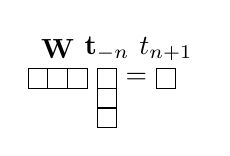
\begin{tikzpicture}
% W matrix
\def\Nx{3}
\def\Ny{1}
\def\cellwidth{0.25}
\foreach \x in {1,...,\Nx} {
    \foreach \y in {1,...,\Ny} {
        \draw [fill=white] (\cellwidth*\x-\cellwidth,\cellwidth*\y-\cellwidth) rectangle ++(\cellwidth,\cellwidth);
    }
}
\draw (\cellwidth*\Nx*0.5, \cellwidth*2) node {$\mathbf{W}$};
% token sequence
\def\Nx{1}
\def\Ny{3}
\def\cellwidth{0.25}
\foreach \x in {1,...,\Nx} {
    \foreach \y in {1,...,\Ny} {
        \draw [fill=white] (\cellwidth*\x+\cellwidth*3.5-\cellwidth,-\cellwidth*\y+\cellwidth) rectangle ++(\cellwidth,\cellwidth);
    }
}
\draw (\cellwidth*0.5+\cellwidth*3.5, \cellwidth*2) node {$\mathbf{t}_{-n}$};
%
\draw (\cellwidth*0.5+\cellwidth*5, \cellwidth/2) node {$=$};
% token output
\draw [fill=white] (\cellwidth+\cellwidth*6.5-\cellwidth,\cellwidth-\cellwidth) rectangle ++(\cellwidth,\cellwidth);
\draw (\cellwidth*0.5+\cellwidth*6.5, \cellwidth*2) node {$t_{n+1}$};
\end{tikzpicture}
\end{minipage}
}
\caption{Masked prediction of time index 4 from time indices 1-3.}
\end{figure}

\marginnote{We depict a sequence of tokens as a vector of cells here, but remember that each cell contains a code vector, and the matrix math here follows \eqn{\ref{eqn:transformers:lin_comb_tokens}} rather than conventional matrix math.}[-2cm]

During training, we will give examples like this:
\begin{align}
    \{t_1, \ldots, t_n\} &\rightarrow t_{n+1}\\
    \{t_1, \ldots, t_{n-1}\} &\rightarrow t_n\\
    \{t_1, \ldots, t_{n-2}\} &\rightarrow t_{n-1}\\
    \ldots
\end{align}

We can make all these predictions at once with a single matrix multiply:
\begin{figure}[h]
\centerline{
\begin{minipage}{.49\linewidth}
\centering
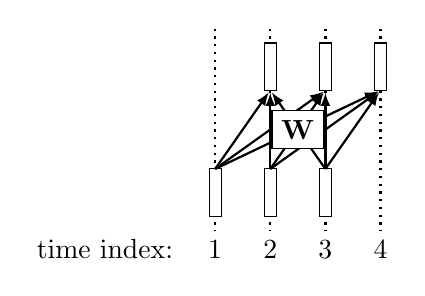
\begin{tikzpicture}
%
\def\Nnodes{3}
\def\Nnodesplusone{4}
\def\layerheight{1.6}
\def\neuronrad{0.3}
\def\neuronstep{0.7}
% time bars
\foreach \x in {1,...,\Nnodesplusone} {
    \draw [dotted, thick] (\neuronstep*\x,-\layerheight*0.5) -- (\neuronstep*\x,\layerheight*1.3);
}
% input sequence
\foreach \x in {1,...,\Nnodes} {
    \draw [fill=white] (\neuronstep*\x-\neuronrad/4,-\neuronrad) rectangle ++(\neuronrad/2,\neuronrad*2);
}
% output target
\foreach \x in {2,...,\Nnodesplusone} {
    \draw [fill=white] (\neuronstep*\x-\neuronrad/4,\layerheight-\neuronrad) rectangle ++(\neuronrad/2,\neuronrad*2);
}
%\draw (\neuronstep*\Nnodes+\neuronstep,\layerheight+\neuronrad*2) node {$t_{n+1}$};
% linear layer
\foreach \xi in {1,...,\Nnodes} {
    \foreach \yi in {2,...,\Nnodesplusone} {
        \ifthenelse{\yi>\xi}{
            \draw [thick] [nn_edge] ($(\neuronstep*\xi,\neuronrad)$) -- ($(\neuronstep*\yi,\layerheight-\neuronrad)$);
        }{}
    }
}
% time steps
\def\tokennames {{"$0$","$1$","$2$","$3$","$4$"}}
\foreach \xi in {1,...,\Nnodesplusone} {
    \pgfmathparse{\tokennames[\xi]};
    \draw ($(\neuronstep*\xi,-\neuronrad*2.4)$) node [fill=white] {\pgfmathresult};
}
\draw ($(-\neuronstep,-\neuronrad*2.4)$) node {time index:};
%
\draw (2.5*\neuronstep,0.5*\layerheight) node[draw,rectangle,fill=white] {$\mathbf{W}$};
%
\end{tikzpicture}
\centering
\end{minipage}
\begin{minipage}{.49\linewidth}
\centering
\begin{tikzpicture}
% W matrix
\def\Nx{3}
\def\Ny{3}
\def\cellwidth{0.25}
\foreach \x in {1,...,\Nx} {
    \foreach \y in {1,...,\Ny} {
        \def\xplusone{\x+1};
        \ifthenelse{\y>\xplusone}{\definecolor{cellfill}{rgb}{1,1,1}}{\definecolor{cellfill}{rgb}{0,0,0}};
        \draw [fill=cellfill] (\cellwidth*\x-\cellwidth,-\cellwidth*\y+\cellwidth) rectangle ++(\cellwidth,\cellwidth);
    }
}
\draw (\cellwidth*\Nx*0.5, \cellwidth*2) node {$\mathbf{W}$};
% token sequence
\def\Nx{1}
\def\Ny{3}
\def\cellwidth{0.25}
\foreach \x in {1,...,\Nx} {
    \foreach \y in {1,...,\Ny} {
        \draw [fill=white] (\cellwidth*\x+\cellwidth*4.5-\cellwidth,-\cellwidth*\y+\cellwidth) rectangle ++(\cellwidth,\cellwidth);
    }
}
\draw (\cellwidth*0.5+\cellwidth*4.5, \cellwidth*2) node {$\tin$};
%
\draw (\cellwidth*0.5+\cellwidth*6, \cellwidth/2) node {$=$};
% token output
\def\Nx{1}
\def\Ny{3}
\def\cellwidth{0.25}
\foreach \x in {1,...,\Nx} {
    \foreach \y in {1,...,\Ny} {
        \draw [fill=white] (\cellwidth*\x+\cellwidth*7.5-\cellwidth,-\cellwidth*\y+\cellwidth) rectangle ++(\cellwidth,\cellwidth);
    }
}
\draw (\cellwidth*0.5+\cellwidth*7.5, \cellwidth*2) node {$\tout$};
\end{tikzpicture}
\end{minipage}
}
\caption{Masked attention to make multiple causal predictions at once. Black cells are masked; they are filled with zeros.}
\end{figure}

This way, one forward pass makes $N$ predictions rather than $1$ prediction. This is equivalent to doing a single next token prediction $N$ times, but it all happens in a single matrix multiply, using the matrix shown on the right.

This kind of matrix is called \textit{causal} because each output index $i$ only depends on input indices $j$ s.t. $j < i$. If \mathbf{W} is an attention matrix, then this strategy is called \textbf{causal attention}. This is a masking strategy where each token can only attend to \textit{previous} tokens in the sequence. This approach can speed things up dramatically, especially when we stack this operation like shown in \fig{\ref{fig:transformers:multilayer_masked_attention}}.
\begin{figure}[h]
\centerline{
\begin{minipage}{.49\linewidth}
\centering
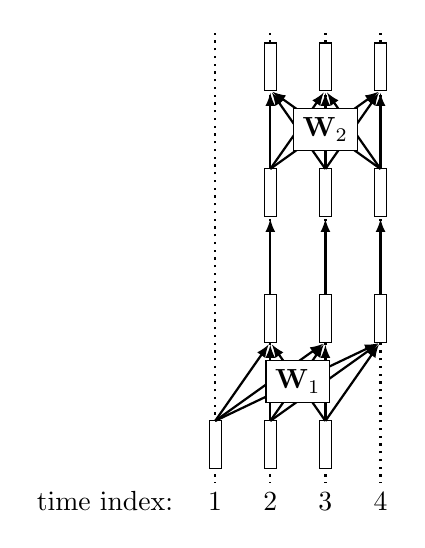
\begin{tikzpicture}
%
\def\Nnodes{3}
\def\Nnodesplusone{4}
\def\layerheight{1.6}
\def\neuronrad{0.3}
\def\neuronstep{0.7}
% time bars
\foreach \x in {1,...,\Nnodesplusone} {
    \draw [dotted, thick] (\neuronstep*\x,-\layerheight*0.5) -- (\neuronstep*\x,\layerheight*3.3);
}
% input sequence
\foreach \x in {1,...,\Nnodes} {
    \draw [fill=white] (\neuronstep*\x-\neuronrad/4,-\neuronrad) rectangle ++(\neuronrad/2,\neuronrad*2);
}
% hidden layer 1
\foreach \x in {2,...,\Nnodesplusone} {
    \draw [fill=white] (\neuronstep*\x-\neuronrad/4,\layerheight-\neuronrad) rectangle ++(\neuronrad/2,\neuronrad*2);
}
%\draw (\neuronstep*\Nnodes+\neuronstep,\layerheight+\neuronrad*2) node {$t_{n+1}$};
% linear layer
\foreach \xi in {1,...,\Nnodes} {
    \foreach \yi in {2,...,\Nnodesplusone} {
        \ifthenelse{\yi>\xi}{
            \draw [thick] [nn_edge] ($(\neuronstep*\xi,\neuronrad)$) -- ($(\neuronstep*\yi,\layerheight-\neuronrad)$);
        }{}
    }
}
% pointwise nonlinearity
\foreach \x in {2,...,\Nnodesplusone} {
    \draw [thick] [nn_edge] (\neuronstep*\x,\layerheight+\neuronrad) -- (\neuronstep*\x,\layerheight*2-\neuronrad);
}
% hidden layer 2
\foreach \x in {2,...,\Nnodesplusone} {
    \draw [fill=white] (\neuronstep*\x-\neuronrad/4,\layerheight*2-\neuronrad) rectangle ++(\neuronrad/2,\neuronrad*2);
}
% linear layer
\foreach \xi in {2,...,\Nnodesplusone} {
    \foreach \yi in {2,...,\Nnodesplusone} {
        \pgfmathparse{\xi-1}
        \ifthenelse{\yi>\pgfmathresult}{
            \draw [thick] [nn_edge] ($(\neuronstep*\xi,2*\layerheight+\neuronrad)$) -- ($(\neuronstep*\yi,3*\layerheight-\neuronrad)$);
        }{}
    }
}
% output layer
\foreach \x in {2,...,\Nnodesplusone} {
    \draw [fill=white] (\neuronstep*\x-\neuronrad/4,\layerheight*3-\neuronrad) rectangle ++(\neuronrad/2,\neuronrad*2);
}
% time steps
\def\tokennames {{"$0$","$1$","$2$","$3$","$4$"}}
\foreach \xi in {1,...,\Nnodesplusone} {
    \pgfmathparse{\tokennames[\xi]};
    \draw ($(\neuronstep*\xi,-\neuronrad*2.4)$) node [fill=white] {\pgfmathresult};
}
\draw ($(-\neuronstep,-\neuronrad*2.4)$) node {time index:};
%
\draw (2.5*\neuronstep,0.5*\layerheight) node[draw,rectangle,fill=white] {$\mathbf{W}_1$};
\draw (3*\neuronstep,2.5*\layerheight) node[draw,rectangle,fill=white] {$\mathbf{W}_2$};
%
\end{tikzpicture}
\end{minipage}
\begin{minipage}{.49\linewidth}
\centering
\begin{tikzpicture}
\def\layerheight{1.6}
% W matrix
\def\Nx{3}
\def\Ny{3}
\def\cellwidth{0.25}
\foreach \x in {1,...,\Nx} {
    \foreach \y in {1,...,\Ny} {
        \ifthenelse{\y<\x}{\definecolor{cellfill}{rgb}{0,0,0}}{\definecolor{cellfill}{rgb}{1,1,1}};
        \draw [fill=cellfill] (\cellwidth*\x-\cellwidth,-\cellwidth*\y+2.5*\layerheight) rectangle ++(\cellwidth,\cellwidth);
    }
}
\draw (\cellwidth*\Nx*0.5, \cellwidth+2.5*\layerheight) node {$\mathbf{W}_2$};
% token sequence
\def\Nx{1}
\def\Ny{3}
\def\cellwidth{0.25}
\foreach \x in {1,...,\Nx} {
    \foreach \y in {1,...,\Ny} {
        \draw [fill=white] (\cellwidth*\x+\cellwidth*4.5-\cellwidth,-\cellwidth*\y+2.5*\layerheight) rectangle ++(\cellwidth,\cellwidth);
    }
}
\draw (\cellwidth*0.5+\cellwidth*4.5, \cellwidth+2.5*\layerheight) node {$\tin$};
%
\draw (\cellwidth*0.5+\cellwidth*6, -\cellwidth/2+2.5*\layerheight) node {$=$};
% token output
\def\Nx{1}
\def\Ny{3}
\def\cellwidth{0.25}
\foreach \x in {1,...,\Nx} {
    \foreach \y in {1,...,\Ny} {
        \draw [fill=white] (\cellwidth*\x+\cellwidth*7.5-\cellwidth,-\cellwidth*\y+2.5*\layerheight) rectangle ++(\cellwidth,\cellwidth);
    }
}
\draw (\cellwidth*0.5+\cellwidth*7.5, \cellwidth+2.5*\layerheight) node {$\tout$};
%
% W matrix
\def\Nx{3}
\def\Ny{3}
\def\cellwidth{0.25}
\foreach \x in {1,...,\Nx} {
    \foreach \y in {1,...,\Ny} {
        \ifthenelse{\y>\x}{\definecolor{cellfill}{rgb}{1,1,1}}{\definecolor{cellfill}{rgb}{0,0,0}};
        \draw [fill=cellfill] (\cellwidth*\x-\cellwidth,-\cellwidth*\y+\cellwidth+0.5*\layerheight) rectangle ++(\cellwidth,\cellwidth);
    }
}
\draw (\cellwidth*\Nx*0.5, \cellwidth*2+0.5*\layerheight) node {$\mathbf{W}_1$};
% token sequence
\def\Nx{1}
\def\Ny{3}
\def\cellwidth{0.25}
\foreach \x in {1,...,\Nx} {
    \foreach \y in {1,...,\Ny} {
        \draw [fill=white] (\cellwidth*\x+\cellwidth*4.5-\cellwidth,-\cellwidth*\y+\cellwidth+0.5*\layerheight) rectangle ++(\cellwidth,\cellwidth);
    }
}
\draw (\cellwidth*0.5+\cellwidth*4.5, \cellwidth*2+0.5*\layerheight) node {$\tin$};
%
\draw (\cellwidth*0.5+\cellwidth*6, \cellwidth/2 + 0.5*\layerheight) node {$=$};
% token output
\def\Nx{1}
\def\Ny{3}
\def\cellwidth{0.25}
\foreach \x in {1,...,\Nx} {
    \foreach \y in {1,...,\Ny} {
        \draw [fill=white] (\cellwidth*\x+\cellwidth*7.5-\cellwidth,-\cellwidth*\y+\cellwidth+0.5*\layerheight) rectangle ++(\cellwidth,\cellwidth);
    }
}
\draw (\cellwidth*0.5+\cellwidth*7.5, \cellwidth*2+0.5*\layerheight) node {$\tout$};
\end{tikzpicture}
\end{minipage}
}
\caption{Multi-layer masked attention achieves causal prediction with a deep net.}
\label{fig:transformers:multilayer_masked_attention}
\end{figure}

Now notice that the output tokens have the property that $\tout[n]$ only depends on $\tin[-n]$. If we apply a causal linear transform again, we will therefore maintain the property that $\tout[n]$ always only depends on $\tin[-n]$. Then, after the first layer, all subsequent layers can use causal attention that is not shifted.


\subsection{Input and output modules}
The transformer also has an input and output module. The input module is the tokenization layer that converts the input signal into a set of tokens. The output module converts the transformed tokens into a target prediction or decision. The input and output modules are specific to the type of input signal and the type of output task. \fig{\ref{fig:transformers:transformer_arch}} shows what the transformer looks like as a whole.
\begin{figure}[h]
    \centerline{
    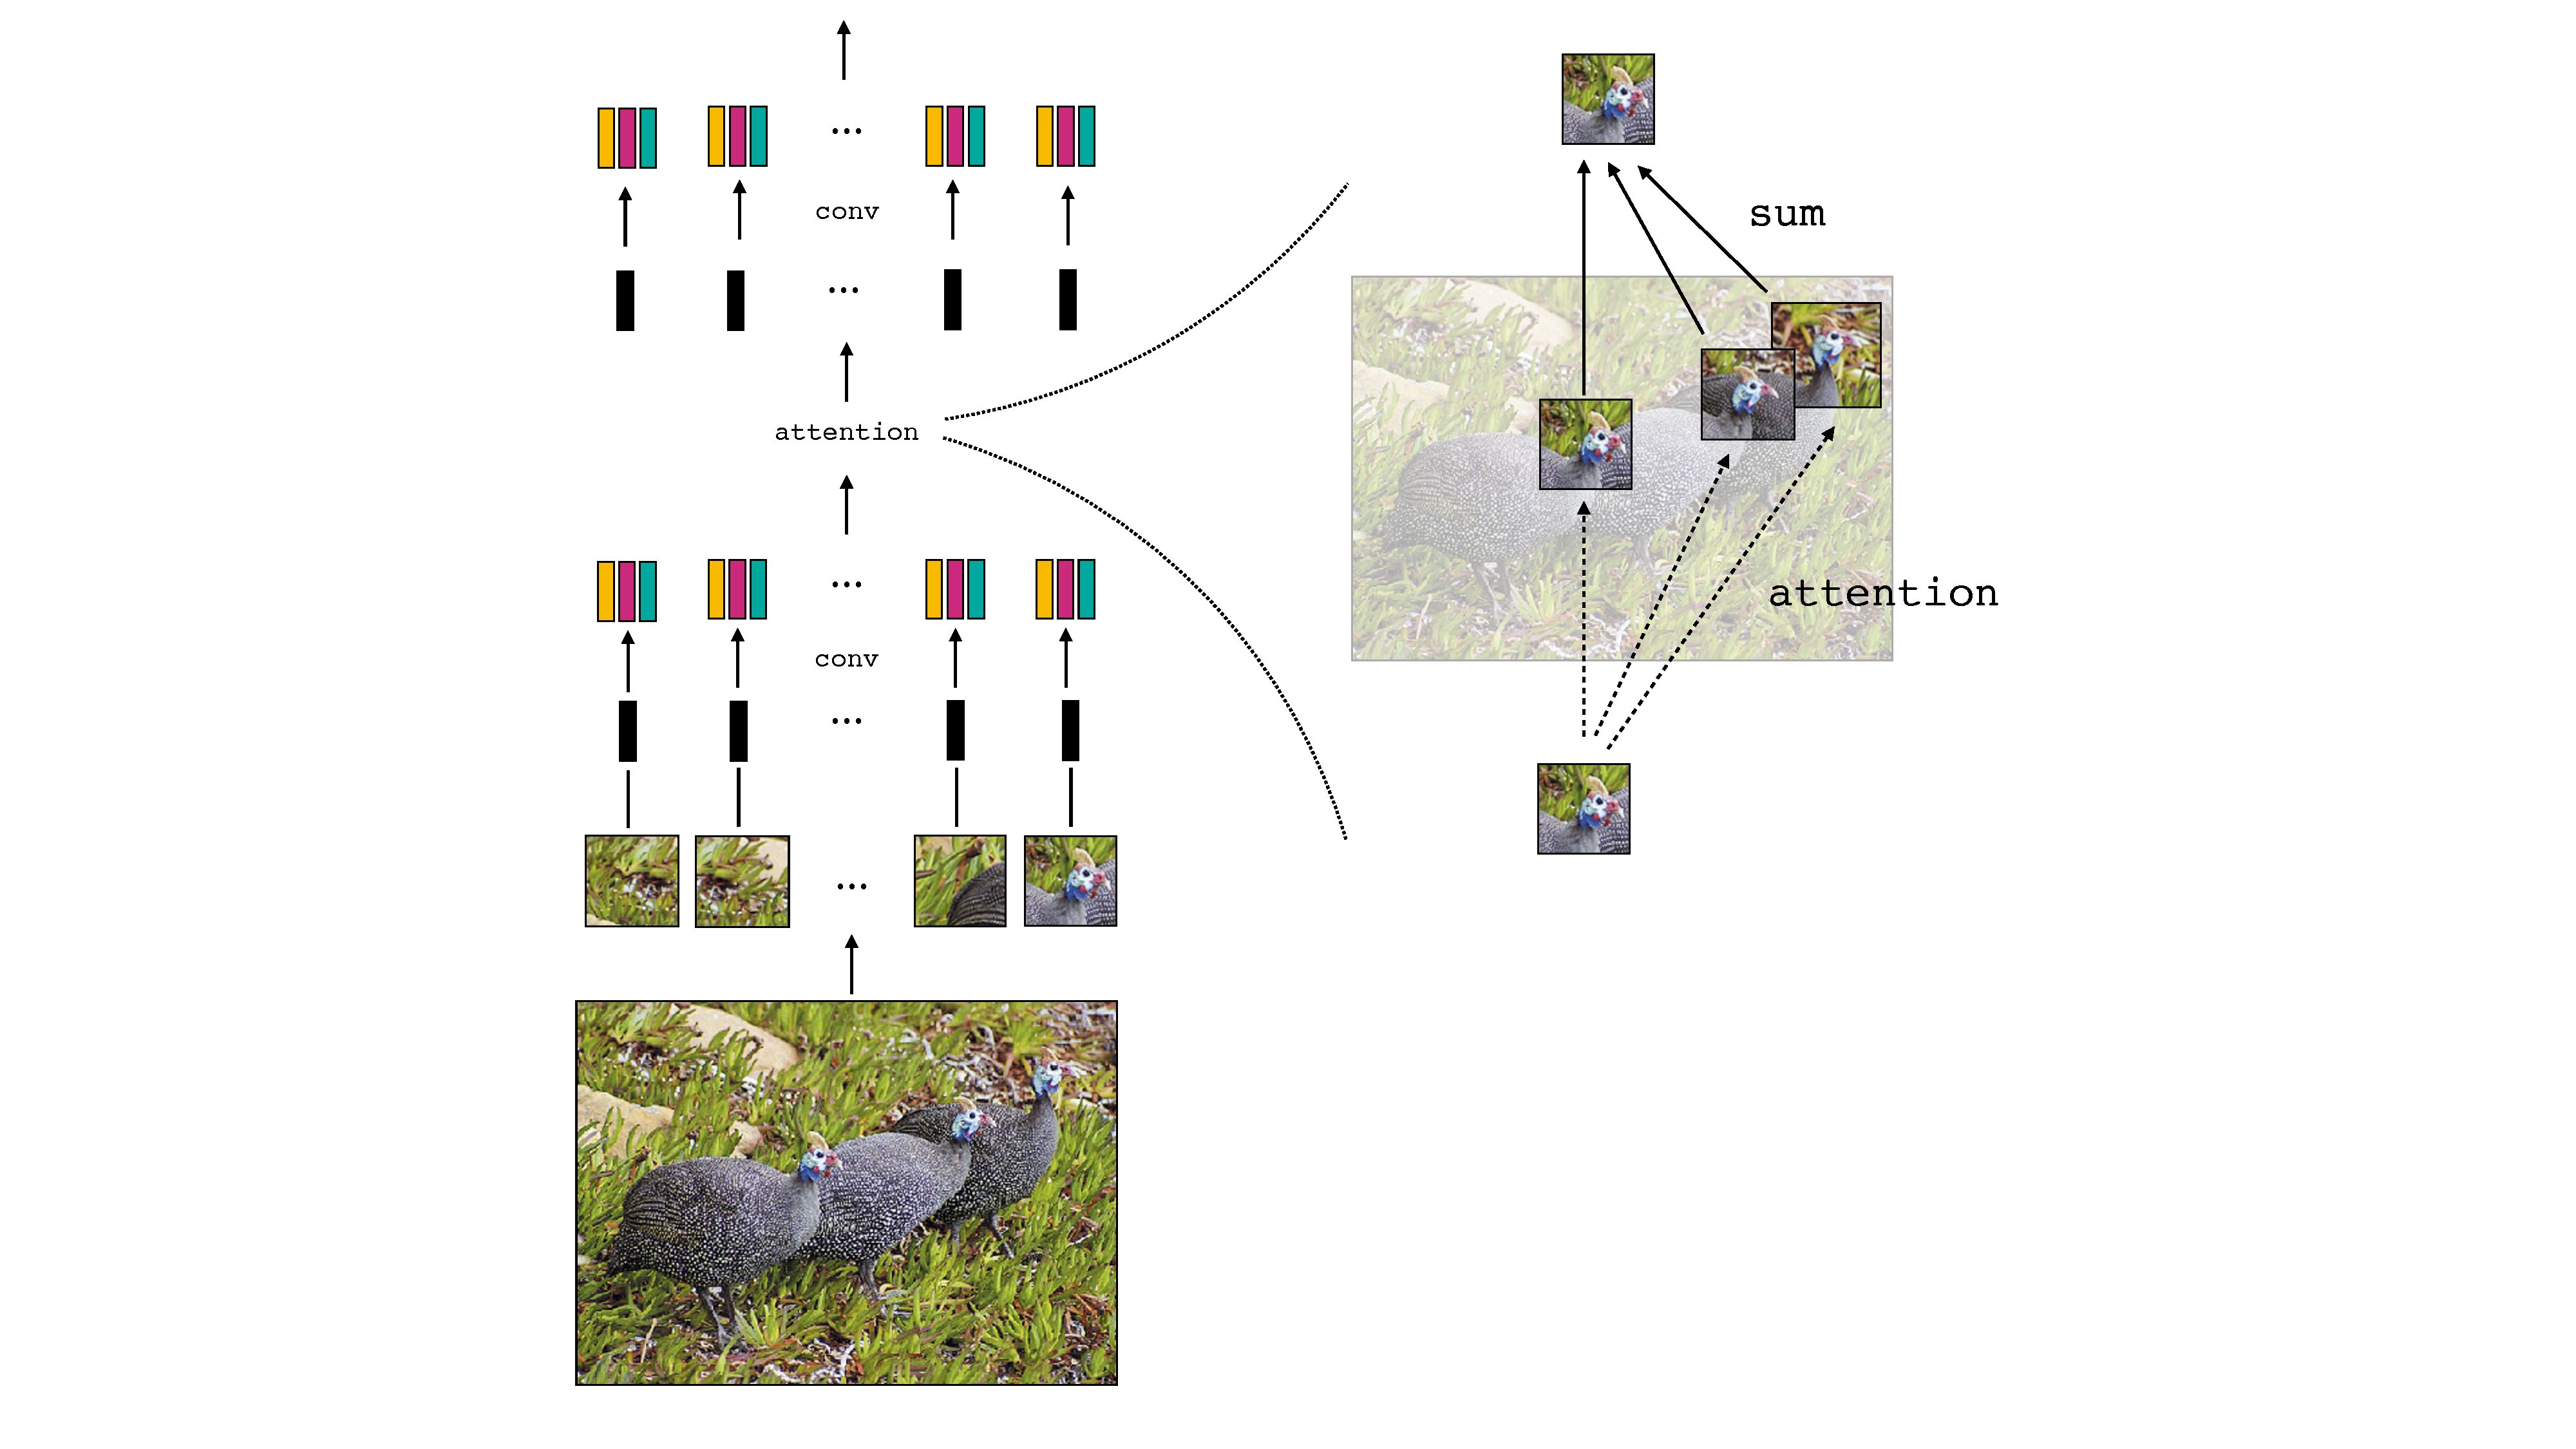
\includegraphics[width=0.8\linewidth]{./figures/transformers/transformer_arch.pdf}
    }
    \caption{Visualizing the full transformer architecture operating on an image.}
    \label{fig:transformers:transformer_arch}
\end{figure}

Notice that most of the operations are familiar from the regular CNNs from Chapter \ref{chapter:convolutional_neural_nets}. As discussed in Section \ref{sec:transformers:modifying_tokens}, the per-token MLP layers are equivalent to CNNs with 1x1 spatial kernels. By a similar argument, it can be shown that the query, key, and value functions are equivalent to 1x1 convs over token code vectors (we leave this as an exercise to the reader). Normalization layers, softmax layers, and residual connections also appear in CNNs. The main novelty of transformers is the self-attention layer. These layers look like fc-layers but are importantly different in two ways:
\begin{enumerate}
    \item They operate over tokens rather than neurons.
    \item The transformation parameters are a function of the input data.
\end{enumerate}

Therefore, we can see that transformers are intimately connected to both MLPs and CNNs, but differ from both in important ways.

\section{Positional encodings}\label{sec:transformers:positional_encodings}
Another idea associated with transformers is {\bf positional encoding}. Operations over tokens in a transformer are permutation equivariant, which means that we can shuffle the positions of the tokens and nothing substantial changes (the only change is that the outputs get permuted). A consequence is that tokens do not naturally encode their position within the representation of the signal. Sometimes we may wish to retain positional knowledge, for example, knowing that a token is a representation of the top region of an image can help us identify that the token is likely to represent sky. Positional encoding concatenates a code representing \textit{position within the signal} onto each token. If the signal is an image, then the positional code should represent the x and y coordinate. However, it need not represent these coordinates as scalars -- more commonly we use a periodic representation of position, where the coordinates are encoded as the vector of values a set of sinusoidal waves take on at each position:
\begin{align}
    \mathbf{p}_x = [\sin(x), \sin(x/B), \sin(x/B^2), \ldots, \sin(x/B^P)]\\
    \mathbf{p}_y = [\sin(y), \sin(y/B), \sin(y/B^2), \ldots, \sin(y/B^P)]
\end{align}
where $x$ and $y$ are the coordinates of the token.

While positional encoding is useful and common in transformers, it is not specific to this architecture. The same kind of encodings can be useful for CNNs as well, as a way to make convolutional filters that are conditioned on position, thereby applying a different weighted sum at each location in the image~\cite{liu2018intriguing}. Positional encodings also appear in many graphics applications, e.g., \cite{mildenhall2020nerf}.


% \section{Transformers: convnets in disguise}
% Before moving on, let's consider an alternative way of understanding this layer. For concreteness, suppose this layer is \texttt{linear}-\texttt{relu}-\texttt{linear}. Suppose the input is a 1D tensor of tokens. As above, we can represent this as a matrix $\Xin$ with each token being a row vector, or you can think of it as a 1D multi-channel signal, with the channels being the columns of $\Xin$. With this last interpretation, $F_{\theta}(\Xin)$ doing? It's an operator you should be very familiar with from previous chapters. Do you see it? Let's work it out step by step.\marginnote{We refer to linear transformations of a token as a ``projection", following common practice in the transformer literature.}[2cm]
% \begin{align}
%     &\Xout = [F_{\theta}(\Xin[1,:]), \ldots, F_{\theta}(\Xin[N,:])]\\
%     \nonumber \\
%     &\text{Per-token MLP:}\nonumber \\
%     &\quad\quad \mathbf{Z} = [\mathbf{W_1}\Xin[1,:] + \mathbf{b}_1, \ldots, \mathbf{W_1}\Xin[N,:] + \mathbf{b}_1] &\quad\quad \triangleleft \quad \texttt{token project}\\
%     &\quad\quad \mathbf{H} = [\texttt{relu}(\mathbf{Z}[1,:]), \ldots, \texttt{relu}(\mathbf{Z}[N,:])] &\quad\quad \triangleleft \quad \texttt{relu}\\
%     &\quad\quad \Xout = [\mathbf{W_2}\mathbf{H}[1,:] + \mathbf{b}_2), \ldots, \mathbf{W_2}\mathbf{H}[N,:] + \mathbf{b}_2] &\quad\quad \triangleleft \quad \texttt{token project}\\
%     \nonumber \\
%     &\text{Equivalent conv net:}\nonumber \\
%     &\quad\quad \mathbf{Z}[:,k] = \sum_c \mathbf{W_1}[c,k] \star \Xin + \mathbf{b}_1[k] \quad \forall k &\quad\quad \triangleleft \quad \texttt{conv}\\
%     &\quad\quad \mathbf{H} = [\texttt{relu}(\mathbf{Z}[1,:]), \ldots, \texttt{relu}(\mathbf{Z}[N,:])] &\quad\quad \triangleleft \quad \texttt{relu}\\
%     &\quad\quad \Xout[:,k] = \sum_c \mathbf{W_2}[c,k] \star \mathbf{H} + \mathbf{b}_2[k] \quad \forall k &\quad\quad \triangleleft \quad \texttt{conv}
% \end{align}
% That's right, it's a convolutional network. Each convolution kernel has spatial size 1 and stride 1. Here we come again across an idea that we emphasized in the chapter on CNNs: the core idea of convolution is just to chop up a signal into chunks and process each chunk idependently and identically. That's exactly what we are doing here with applying an MLP to each token in a ``pointwise" fashion, so clearly what we are doing is just applying a convolution network by a different name. 


% \section{Other uses of attention}

% It is also possible to attend between different sets of tokens, where queries produced by one set match with keys produced by a different set. Such a layer is simply called an {\bf attention layer} rather than a self-attention layer.

%A transformer is a CNN for which the filter weights are \textit{dynamic}. This means that the weights on each layer are not fixed during each forward pass but instead determined by the previous layer's activations.


\begin{figure}[t]
    \centerline{
        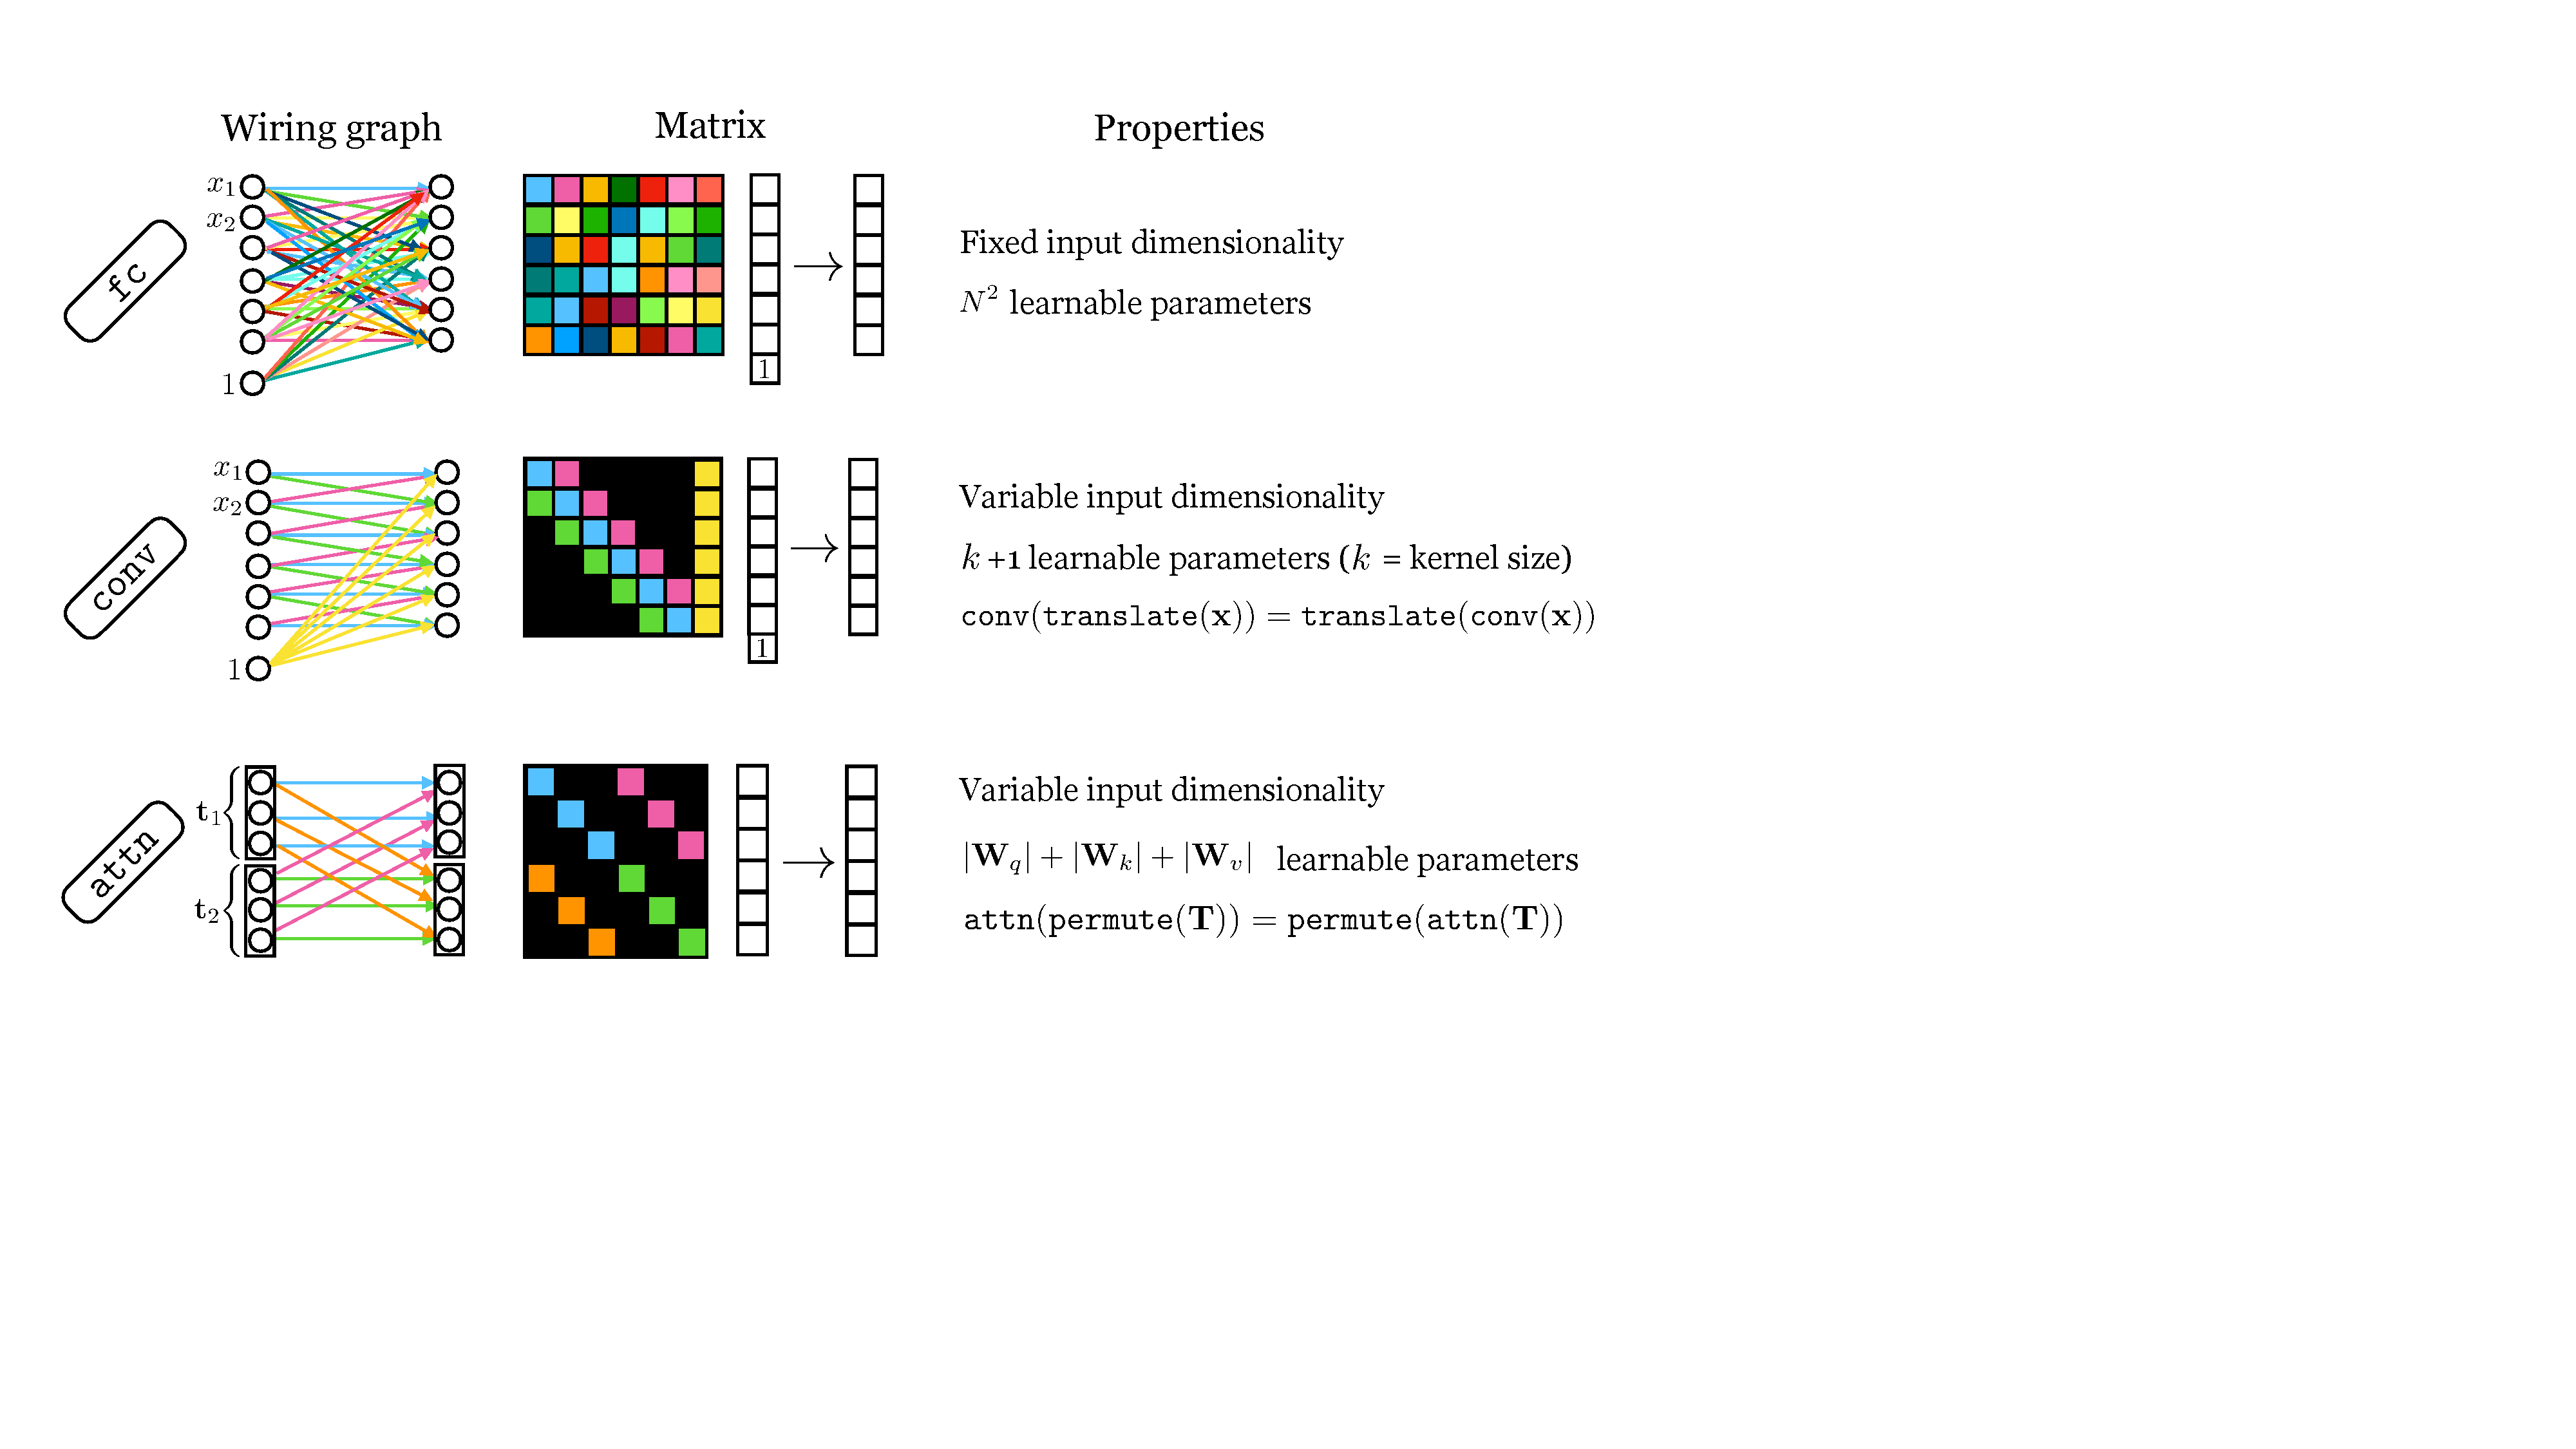
\includegraphics[width=1.0\linewidth]{figures/transformers/affine_layer_comparison.pdf}
    }
    \caption{Comparing different kinds of layers that all represent an affine transformation between the inputs and outputs.}
  \label{fig:transformers:affine_layer_comparison}
\end{figure}

\section{Comparing fc, conv, and attn}

Many layers in deep nets are special kinds of affine transformations. Three we have seen so far are fc layers, conv layers, and self-attention layers. All these layers are alike in that their forward pass can be written as $\Xout = \mathbf{W}\Xin + \mathbf{b}$ for some matrix $\mathbf{W}$ and some vector $\mathbf{b}$. In conv and attn layers, $\mathbf{W}$ and $\mathbf{b}$ are determined as some function of the input $\Xin$. In conv layers this function is very simple: just make a Toeplitz matrix that repeats the convolutional kernel(s) to match the dimensionality of $\Xin$. In self-attention layers the function that determines $\mathbf{W}$ is a bit more involved, as we saw above, and typically we don't use biases $\mathbf{b}$.

Each of these layers can be represented as a matrix, and examining the structure in these matrices can be a useful way to understand their similarities and differences. The matrix for an fc layer is full rank, whereas the matrices for conv and self-attention layers have low-rank structure, but different kinds of low-rank structure. In \fig{\ref{fig:transformers:affine_layer_comparison}}, we show what these matrices look like, and also catalogue some of the other important properties of each of these layers.


\section{Concluding remarks}
As of this writing, transformers are the dominant architecture in computer vision and in fact in most fields of AI. They combine many of the best ideas from earlier architectures -- convolutional ``token-wise'' processing, residual connections, relu nonlinearities and normalization layers -- with several newer innovations -- vector-valued tokens, attention layers, and positional codes. Transformers can also be considered as a special case of a \textbf{graph neural network} or \textbf{GNN}. We do not have a separate chapter on GNNs in this book since GNNs, other than transformers, are not yet popular in computer vision. GNNs are a very general class of architecture for processing \textit{sets} by forming a graph of operations over the set. A transformer is doing exactly that: it takes an input set of tokens and, layer by layer, applies a network of transformations over that set, until after enough layers, a final representation or prediction is read out.